% !TeX root = probability.tex

%%%%%%%%%%%%%%%%%%%%%%%%%%%%%%%%%%%%%%%%%%%%%%%%%%%%%%%%%%%%%%%%

\documentclass[12pt,a4paper,leqno]{article}

\usepackage{verbatim}
\usepackage{url}
\usepackage{fancyhdr}
\usepackage{graphicx}
\usepackage{bm}

\graphicspath{{../images/}}

% TikZ package
\usepackage{tikz}
\usetikzlibrary{arrows.meta,shapes}
\tikzset {>=Stealth}

% Polyglossia Hebrew (main) and English (other)
\usepackage{polyglossia}  
\setmainlanguage{hebrew}
\setotherlanguage{english}

% Fonts: David for Hebrew, Palatino/Courier for English
\newfontfamily{\hebrewfont}{David}[Script=Hebrew]
\newfontfamily{\englishfont}{Palatino Linotype}
\newfontfamily{\englishfonttt}{Courier New}
\newfontfamily{\hebrewfonttt}{Courier New}

% Abbreviations for backwards compatibility with babel
\renewcommand*{\L}[1]{\textenglish{\small #1}}
\newcommand*{\R}[1]{\texthebrew{#1}}

% Use fancyhdr to make all page numbers uniform
\pagestyle{fancy}
\fancyhead{}
\renewcommand{\headrulewidth}{0pt}
\renewcommand{\footrulewidth}{0pt}
\fancyfoot[C]{$\thepage$}

% Displaystyle for fractions and combinations
\newcommand*{\disfrac}[2]{\displaystyle\frac{#1}{#2}}
\newcommand*{\dischoose}[2]{\displaystyle{#1 \choose #2}}

\newcommand*{\bover}[1]{\bm{\overline{#1}}}
\newcommand*{\erh}[1]{\renewcommand{\arraystretch}{#1}}

% Reduce space around c column in eqnarray*
\newenvironment{eqn}
  {\addtolength{\arraycolsep}{-3pt}\begin{eqnarray*}}
  {\end{eqnarray*}}
  
% Reduce space around c column in eqnarray with labels
\newenvironment{eqnlabels}
  {\addtolength{\arraycolsep}{-3pt}
   \begin{eqnarray}}
  {\end{eqnarray}}

% Use english equation numbers in hebrew document
\renewcommand{\theequation}{\L{\arabic{equation}}}

% Allow pages with larger floats
\renewcommand{\floatpagefraction}{.8}

% Layout
\textwidth=155mm
\textheight=230mm
\topmargin=0pt
\headheight=0pt
\oddsidemargin=0mm
\evensidemargin=0mm
\headsep=0pt
\parindent=0pt
\renewcommand{\baselinestretch}{1.1}
\setlength{\parskip}{0.3\baselineskip plus 1pt minus 1pt}

%\includeonly{bet}

\begin{document}
% !TeX root = probability.tex

\selectlanguage{hebrew}

\thispagestyle{empty}

\begin{center}
\textbf{\LARGE בחינות בגרות בהסתברות}
\end{center}

\bigskip
\bigskip

\begin{center}
\textbf{\Large מוטי בן-ארי}

\bigskip

\url{http://www.weizmann.ac.il/sci-tea/benari/}
\end{center}

\begin{center}	
\begin{bfseries}
\bigskip
\bigskip

\R{גרסה} \L{1.0} 

\bigskip

\today

\end{bfseries}
\end{center}

\vfill

\selectlanguage{english}

\begin{small}
\begin{center}
\copyright{}\ 2022 \R{מוטי בן-ארי}
\end{center}

This work is licensed under a Creative Commons Attribution-ShareAlike 4.0 International License:
\url{http://creativecommons.org/licenses/by-sa/4.0/}.
\end{small}

\bigskip

\begin{center}

\includegraphics[width=.2\textwidth]{../by-sa.png}
\end{center}

\newpage

\selectlanguage{hebrew}

\thispagestyle{empty}

\tableofcontents

\newpage

\section*{מבוא}
\addcontentsline{toc}{section}{\large מבוא}

חוברת זו כוללת פתרונות לכל השאלות על הסתברות של בחינות הבגרת (שאלון 
$806 / 581$)
מהשנים תשע"ד עד תשפ"ב. 
הדגשים בפתרונות הם:
\begin{itemize}
\item 
זיהוי מוקפד של המאורעות.

\item
הנמקה של בחירת שיטות לחישוב ולהצגת החישוב: עץ, טבלה, ברנולי, בינום, עם דגש מיוחד על הבנת הניסוחים הרבים המכוונים להסתברות מותנית.
\item
לא הססתי לכלול תיאור של מקרים בהם הסתבכתי בפתרון!
\item
בסוף החוברת נמצא סעיף "המלצות" המסכם לקחים מהפתרונות.
\item
החוברת מופצת עם רישיון המאפשר העתקה חופשית. ניתן להוריד את המסמכים ב-%
\L{PDF}
מ:
\begin{center}
\selectlanguage{english}
\url{https://github.com/motib/bagrut}
\selectlanguage{hebrew}
\end{center}
שם נמצא גם קוד המקור ב-%
\L{\LaTeX{}}.
המסמך בעברית ויש להשתמש ב-%
\L{\XeLaTeX{}}
ולא ב-%
\L{pdflatex}.
\end{itemize}

\textbf{סימון המאורעות}
אני מקפיד עם סימון מאורעות כי לדעתי זה מקל על הבנת החישובים לעומת שימוש בשפה טבעית. הסימון גם מעודד חשיבה לזיהוי מוקפד של המאורעות. למשל:
\begin{quote}
נסמן ב-%
$N$ \L{(neta)}
ניצחון של נטע במשחק.
\end{quote}
כאשר מבקשים גם את מספר הנצחונות של נטע נשתמש בסימון כגון
$N=4$
או
$N\geq 5$.\footnote{$N\geq 5$
הוא למעשה משתנה אקראי שערכו גדול או שווה ל-$5$, אבל המונח לא נמצא בתכנית הלימודים.}


% !TeX root = probability.tex

%%%%%%%%%%%%%%%%%%%%%%%%%%%%%%%%%%%%%%%%%%%%%%%%%%%%%%%%%%%%%%


\addcontentsline{toc}{section}{\large בחינות ופתרונות}

\section{קיץ תשפ"ב מועד ב}

\begin{center}
\selectlanguage{english}
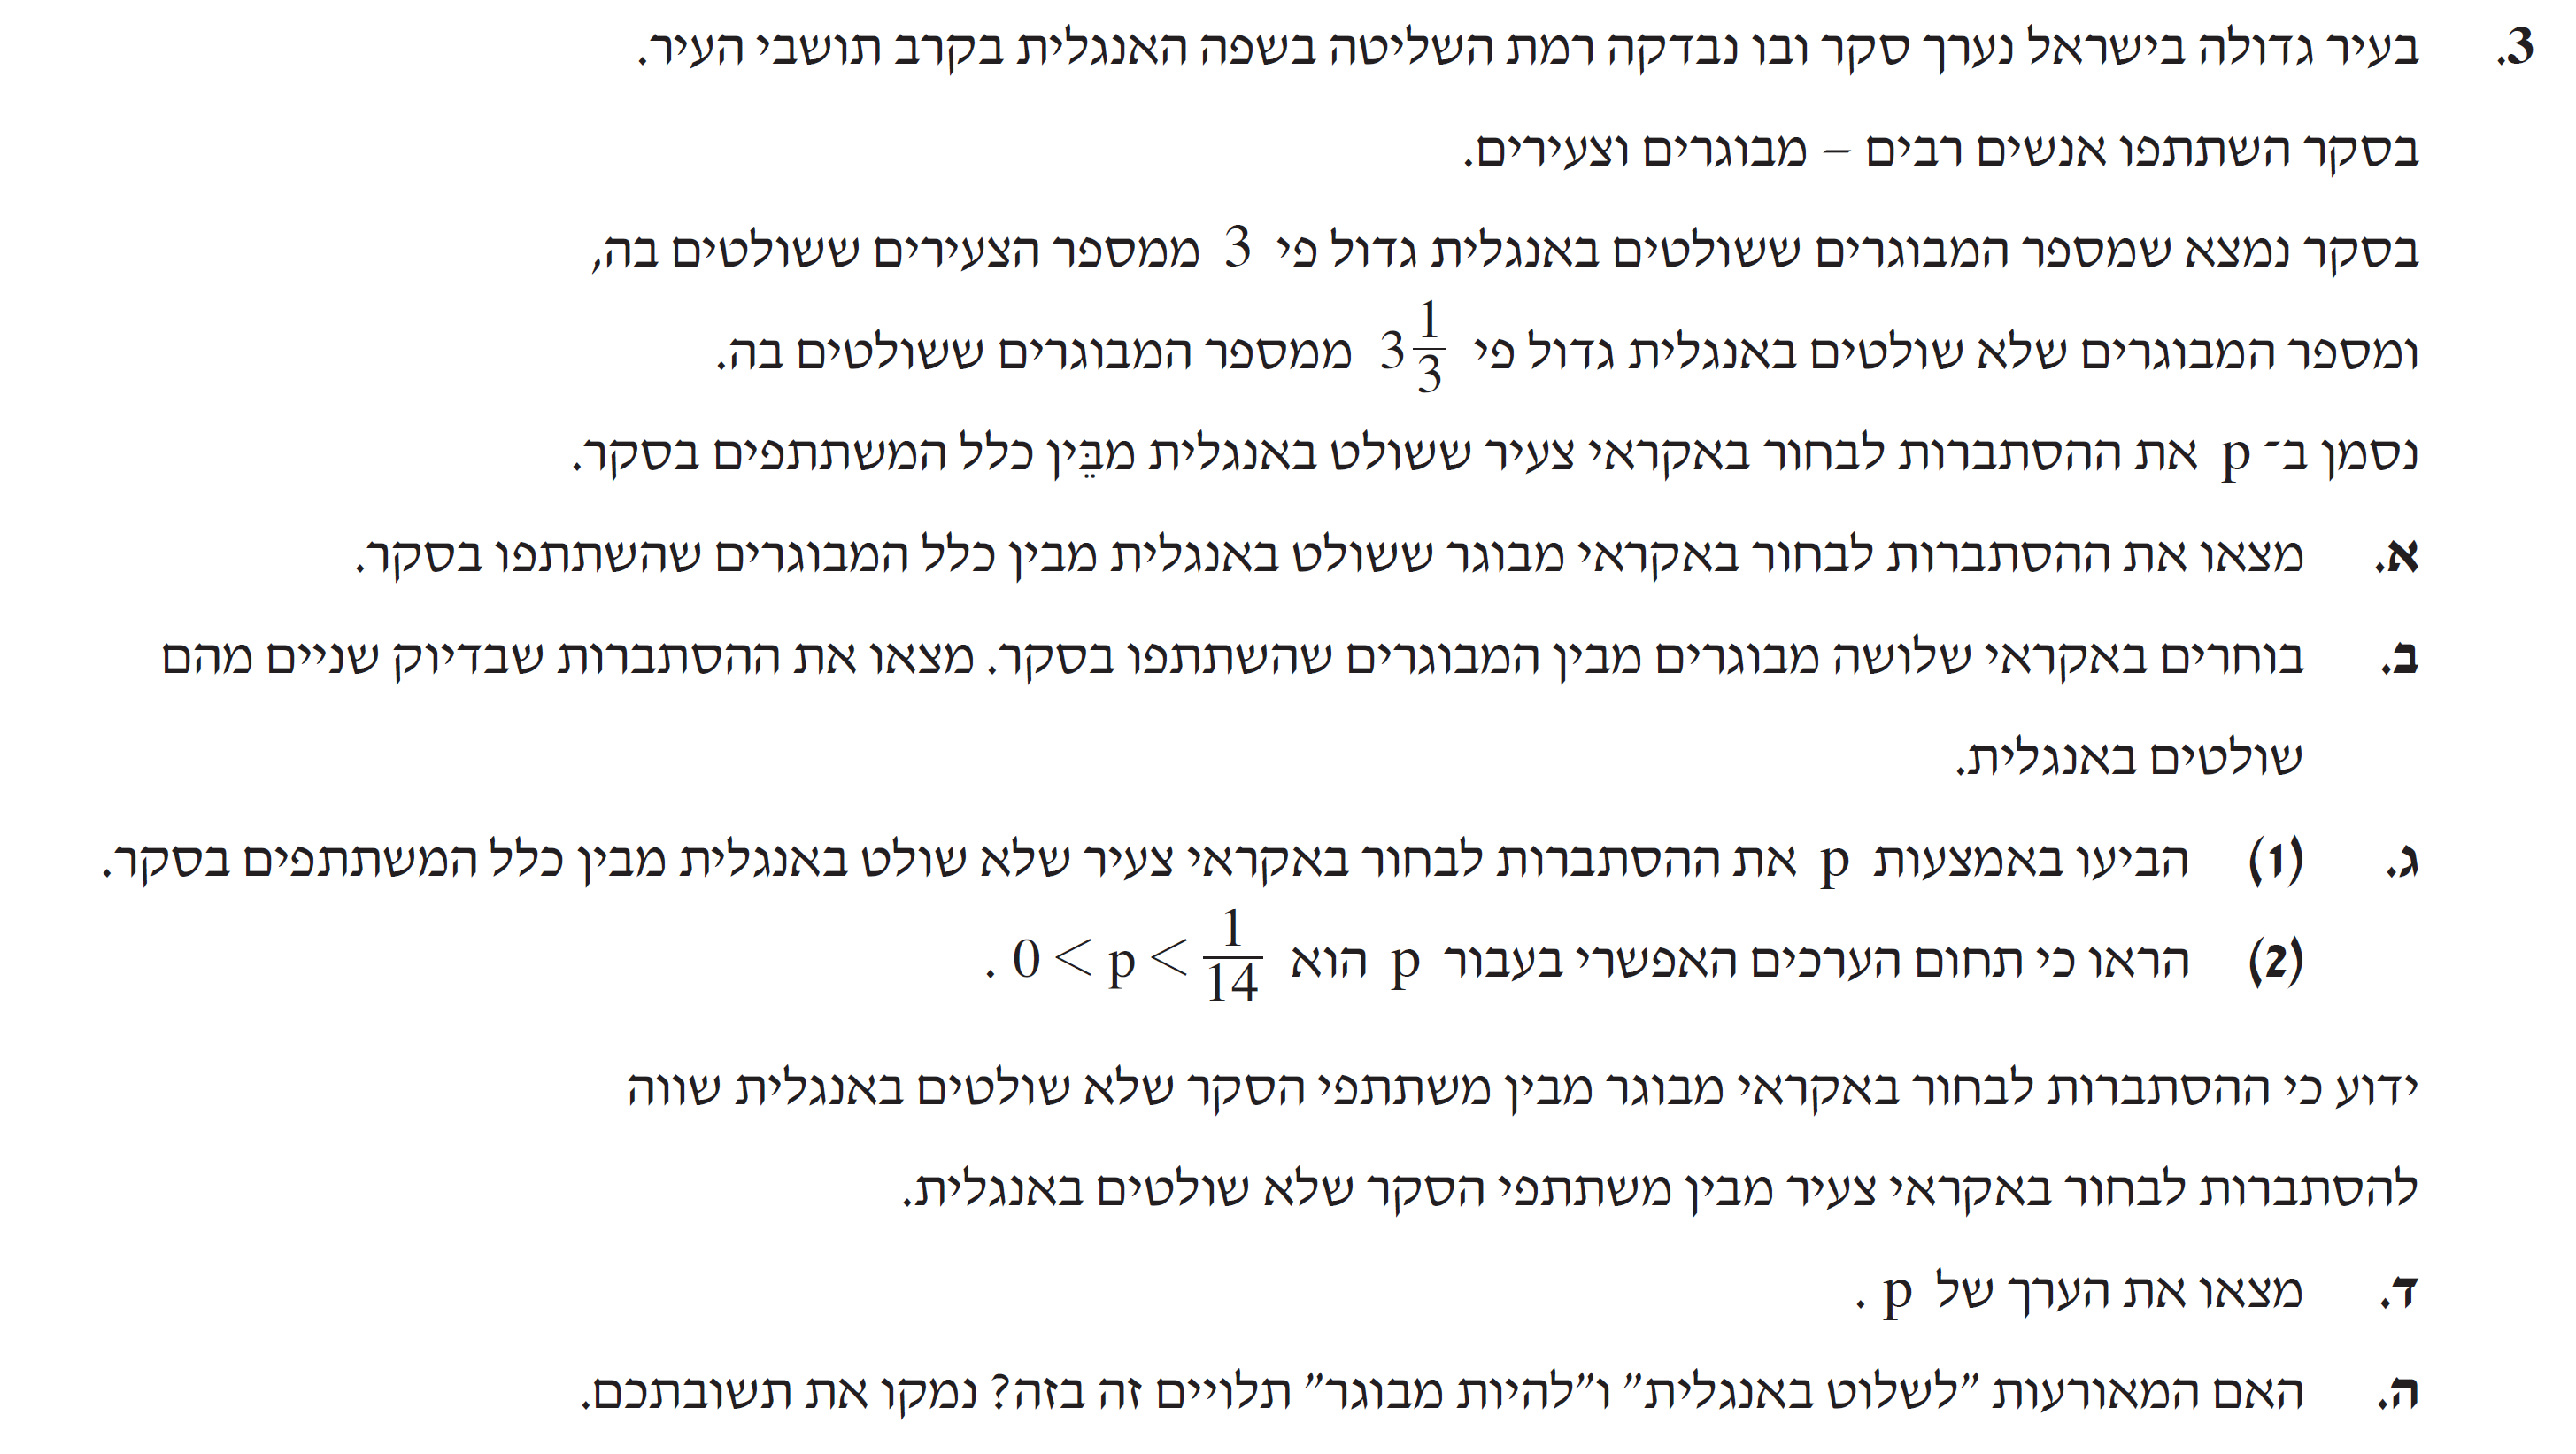
\includegraphics[width=\textwidth]{summer-2022b-3}
\end{center}

נסמן ב-%
$M$ \L{(mevugar)}
את המאורע של מבוגר ונסמן ב-%
$A$ \L{(anglit)}
את המאורע של שליטה באנגלית. השאלה שואלת על שני סוגים של מאורעות ולכן נארגן את המידע בטבלה. נתון הסימון
$p=P(\overline{M}\cap A)$.
\begin{quote}
אפשר לחשוב שניסוח "מבין" מכוון להסתברות מותנית, אבל בגלל שהניסוח "מבין כלל המשתתפים בסקר" מתייחס ל"כולם", אין אף משתתף שלא משתתף! אם רוצים אפשר לחשב הסתברות מותנית, כאשר נסמן את "כלל המשתתפים בסקר ב-%
$K$
ואז:
\begin{eqn}
P(K)&=&P(M\cup \overline{M})=P(A\cup \overline{A})=1\\
P((\overline{M}\cap A)/K)&=&
\frac{P((\overline{M}\cap A)\cap K)}{P(K)}=P(\overline{M}\cap A)\,.
\end{eqn}
\end{quote}

נתון גם ש-%
$P(M\cap A)=3P(\overline{M}\cap A)$
ולכן
$P(M\cap A)=p$,
ונתון ש-%
$P(M\cap \overline{A})=\frac{10}{9}P(M\cap A)$
ולכן
$P(M\cap \overline{A})=10p$.
ביחד עם ההסתברויות המשלימות נוכל למלא את כל התאים בטבלה.
\begin{center}
\begin{tikzpicture}[scale=1.25]
\draw (0,0) grid[xstep=1.5] (4.5,3);
\node at (3.75,3.3) {$M$};
\node at (2.25,3.3) {$\overline{M}$};
\node at (5,2.5) {$A$};
\node at (5,1.5) {$\overline{A}$};

\node at (3.75,2.5) {$3p$};
\node at (2.25,2.5) {$p$};
\node at (0.75,2.5) {$4p$};

\node at (3.75,1.5) {$10p$};
\node at (2.25,1.5) {$1-14p$};
\node at (0.75,1.5) {$1-4p$};

\node at (0.75,0.5) {$1$};
\node at (2.25,0.5) {$1-13p$};
\node at (3.75,0.5) {$13p$};
\end{tikzpicture}
\end{center}

\textbf{סעיף א}

\[
P(M\cap A/M)=\frac{P((M\cap A)\cap M)}{P(M)}=\frac{P(M\cap A)}{P(M)}=\frac{3p}{13p}=\frac{3}{13}\,,
\]
כי אם המשתתף נמצא ב-%
$M\cap A$
הוא כמובן נמצא גם ב-%
$M$.

\textbf{סעיף ב}

"מבין" מכוון להסתברות מותנית ו-"בדיוק" מכוון לנוסחת ברנולי. נשתשמש בתוצאה של הסעיף הקודם:
\[
P((M\cap A)=2/M=3)={3\choose 2}\left(\frac{3}{13}\right)^2
\left(\frac{10}{13}\right)^1=
\frac{270}{2197}=0.1229\,.
\]

\textbf{סעיף ג 1}

מהטבלה
$P(\overline{M}\cap A)=1-14p$.

\textbf{סעיף ג 2}

ההסתברות חייבת להיות בין אפס לאחד. מ-%
$0<1-14p$
מתקבל
$p<1/14$,
ומ-%
$1-14p<1$
מתקבל
$p>0/14=0$.

\textbf{סעיף ד}

כמו בדיון לעיל, "ידוע" לא מכוון להסתברות מותנית:
\begin{eqn}
P(M\cap \overline{A})&=&P(\overline{M}\cap \overline{A})\\
10p&=&1-14P\\
p&=&1/24\,.
\end{eqn}

\textbf{סעיף ה}

נבדוק אם
$P(M\cap A)=P(M)P(A)$:
\begin{eqn}
P(M\cap A)&=& 3p=3/24=1/8\\
P(M)P(A)&=&13p\cdot 4p=52/576=0.72/8\,.
\end{eqn}
הערכים שונים ולכן ההסתברויות תלויות זו בזו.

%%%%%%%%%%%%%%%%%%%%%%%%%%%%%%%%%%%%%%%%%%%%%%%%%%%%%%%%%%%%%

\newpage

\section{קיץ תשפ"ב מועד א}

\begin{center}
\selectlanguage{english}
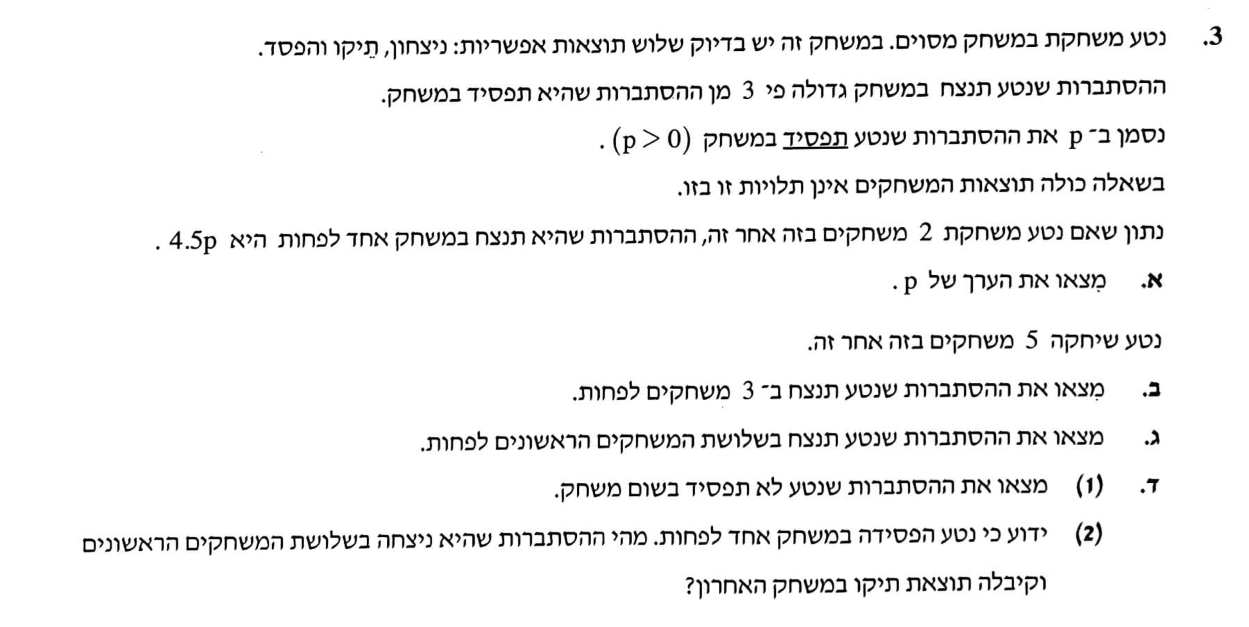
\includegraphics[width=\textwidth]{summer-2022a-3}
\end{center}

נסמן ב-%
$N$ \L{(nitzahon)},
$T$ \L{(teku)},
$H$ \L{(hefsade)}
את המאורעות של ניצחון, תיקו והפסד, בהתאמה. נתון ש-%
$P(H)=p$
ו-%
$P(N)=3p$.
לפי הסתברות משלימה
$P(T)=1-4p$.

\textbf{סעיף א}

ההסתברות לניצחון אחד לפחות היא המשלימה להסתברות לא לנצח פעמיים שהיא ההסתברות להפסד או תיקו פעמיים. לפי הנתון הסתברות זו היא
$4.5p$
ו-%
$p>0$:
\begin{eqn}
1-(p+(1-4p))^2&=&\tfrac{9}{2}p\\
1-(1-6p+9p^2)&=&\tfrac{9}{2}p\\
9p^2&=&\tfrac{3}{2}p\\
p&=&\tfrac{1}{6}\,.
\end{eqn}
מכאן ש-%
$P(N)=\frac{1}{2}, P(T)=\frac{1}{3}$.

\textbf{סעיף ב}

"לפחות" מכוון לנוסחת ברנולי. שימו לב שכאשר ההסתברות היא 
$\frac{1}{2}$:
\[
\left(\frac{1}{2}^k\right)\left(1-\frac{1}{2}\right)^{n-k}=\left(\frac{1}{2}\right)^n\,,
\]
ולכן ההסתברות היא סכום המקדמים הבינומיים כפול 
$\left(\frac{1}{2}\right)^5$:
\[
P(N=3)=\frac{1}{32}\left({5\choose 3}+{5\choose 4}+{5\choose 5}\right)=\frac{16}{32}=\frac{1}{2}\,.
\]

\textbf{סעיף ג}

ההסתברות המבוקשת היא ההסתברות לנצח בשלושה משחקים ברציפות שהיא
$\left(\frac{1}{2}\right)^2=\frac{1}{8}$
כפול ההסתברות לניצחון או תיקו או הפסד בשני משחקים ברציפות שהיא
$1\cdot 1$,
כי שלושת התוצאות הללו מכסות את כל האפשריות. לכן התשובה היא
$\frac{1}{8}$.

\textbf{סעיף ד 1}

ההסתברות שנטע לא תפסיד היא
$1-\frac{1}{6}=\frac{5}{6}$,
ההסתברות המשלימה להסתברות שהיא תפסיד. ההסתברות המבוקשת היא:
\[
P(\overline{H}=5)=\left(\frac{5}{6}\right)^5=\frac{3125}{7776}=0.4019.
\]

\textbf{סעיף ד 2}

מאוד מפתה להבין את השאלה בצורה מוטעית: אם נטע מנצחת בשלושת המשחקים הראשונים ומשיגה תיקו בחמישי, אין ברירה אלא שהיא תפסיד את הרביעי וההסתברות היא:
\[
\left(\frac{1}{2}\right)^3\cdot \frac{1}{6}\cdot \frac{1}{3}=\frac{1}{144}\,.
\]
אבל "ידוע" מכוון להסתברות מותנית וההסתברות שחישבנו מתייחס לחלק מכל התוצאות האפשריות ולא רק מאלו שנטע הפסידה משחק אחד לפחות. ההסתברות המבוקשת היא:
\[
P(N=1,N=2,N=3,T=5/H\geq 1)=\frac{P(N=1,N=2,N=3,T=5\cap H\geq 1)}{P(H\geq 1)}\,.
\]
המונה היא ההסתברות
$\frac{1}{144}$
שבדיוק חישבנו והמכנה הוא ההסתברות
$\frac{3125}{7776}$
שחישבנו בסעיף ד 1. ההסתברות המבוקשת היא:
\[
P(N=1,N=2,N=3,T=5/H\geq 1)=\frac{1/144}{3125/7776}=
\frac{7776}{144\cdot 4651}=\frac{54}{4651}=0.0116\,.
\]

%%%%%%%%%%%%%%%%%%%%%%%%%%%%%%%%%%%%%%%%%%%%%%%%%%%%%%%%%

\newpage

\section{חורף תשפ"ב}

\begin{center}
\selectlanguage{english}
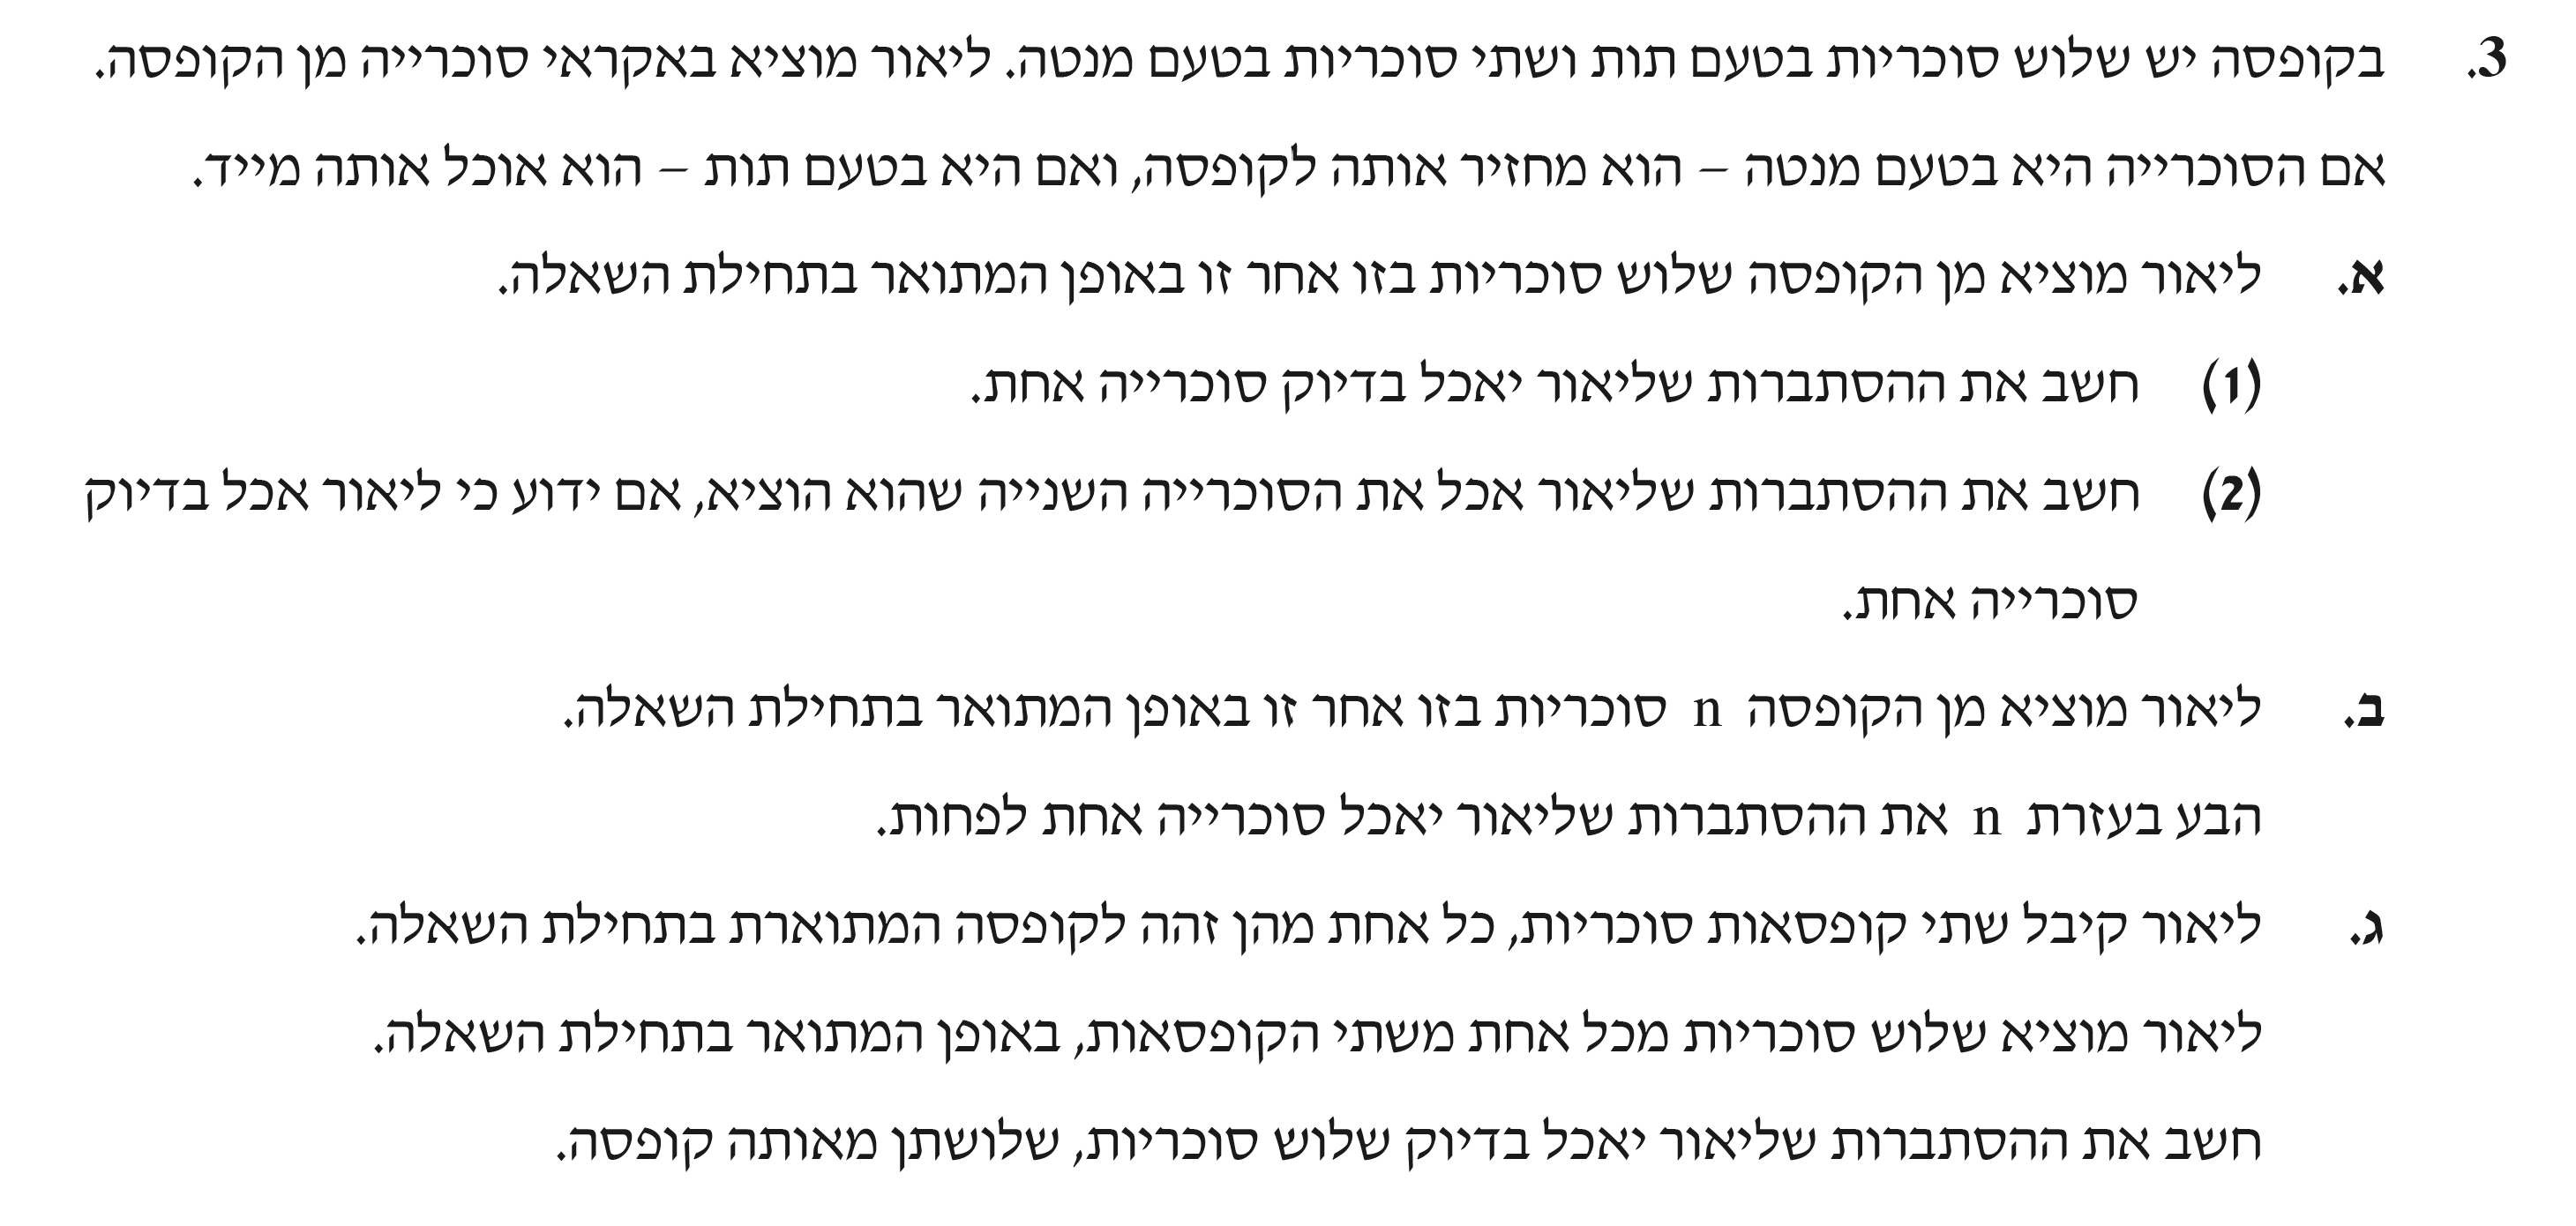
\includegraphics[width=\textwidth]{winter-2022-3}
\end{center}

השאלה שואלת על סדרה של מאורעות ולכן נארגן את המידע בעץ. בצמתים מוסמנים במספר הסוכריות באותו מצב
$(T, M)$,
והקשתות מסומנות בסוג הסוכריה שנשלף וההסתברותה.

\begin{center}
\begin{tikzpicture}
  [grow=right,
   level 1/.append style=
     {level distance=6em,sibling distance=10em},
   level 2/.append style=
     {level distance=6em,sibling distance=5em},
   level 3/.append style=
     {level distance=6em,sibling distance=3em}
  ]
  \node[left] {$\scriptstyle (3,2)$}
    child {node [right] {$\scriptstyle (3,2)$}
      child {node[right]  {$\scriptstyle (3,2)$}
        child {node[right]  {$\scriptstyle (3,2)$}
            edge from parent
            node [below] {$\scriptstyle M,\,2/5$}
        }
        child {node[right] {$\scriptstyle (2,2)$}
            edge from parent 
            node [above] {$\scriptstyle T,\,3/5$}
        }
        edge from parent
        node [below,xshift=-6pt] {$\scriptstyle M,\,2/5$}
      }
      child {node[right]  {$\scriptstyle (2,2)$}
        child {node[right]  {$\scriptstyle (2,2)$}
            edge from parent 
            node [below] {$\scriptstyle M,\,2/4$}
        }
        child {node[right] {$\scriptstyle (1,2)$}
            edge from parent
            node [above] {$\scriptstyle T,\,2/4$}
        }
        edge from parent
        node [above] {$\scriptstyle T,\,3/5$}
      }
      edge from parent
      node [below,,xshift=-10pt] {$\scriptstyle M,\, 2/5$}
    }
    child {node [right] {$\scriptstyle (2,2)$}
      child {node[right]  {$\scriptstyle (2,2)$}
        child {node[right]  {$\scriptstyle (2,2)$}
            edge from parent 
            node [below] {$\scriptstyle M,\,2/4$}
        }
        child {node[right] {$\scriptstyle (1,2)$}
            edge from parent 
            node [above] {$\scriptstyle T, \,2/4$}
        }
        edge from parent
        node [below,xshift=-4pt] {$\scriptstyle M,\, 2/4$}
      }
      child {node[right]  {$\scriptstyle (1,2)$}
        child {node[right]  {$\scriptstyle (1,2)$}
            edge from parent 
            node [below] {$\scriptstyle M, \,2/3$}
        }
        child {node[right] {$\scriptstyle (0,2)$}
            edge from parent 
            node [above] {$\scriptstyle T,\, 1/3$}
        }
        edge from parent node [above] {$\scriptstyle T,\, 2/4$}
      }
      edge from parent
      node [above,xshift=-6pt] {$\scriptstyle T, \,3/5$}
    };
\end{tikzpicture}
\end{center}

\textbf{סעיף א 1}

הניסוי מתחיל עם שלוש סוכריות. ליאור אוכל רק סוכריות תות ולכן ההסתברות שהוא יאכל רק אחת היא סכום ההסתברויות לאורך המסלולים המובילים למצבים המסומנים
$(2,k)$.

אם הוא שוךף סוכריית מנטה הוא לא יאכל אותה ולכן חייב להיות
$k=2$.
יש שלושה מסלולים, הרביעית, ששית ושביעית (מלמעלה):
\begin{eqn}
P((2,2))&=&
\frac{3}{5}\cdot\frac{2}{4}\cdot\frac{2}{4}+
\frac{2}{5}\cdot\frac{3}{5}\cdot\frac{2}{4}+
\frac{2}{5}\cdot\frac{2}{5}\cdot\frac{3}{5}=\frac{183}{500}=0.366\,.
\end{eqn}

\textbf{סעיף א 2}

נסמן ב-%
$A$ \L{(akhal)}
את המאורע של אכילת סוכרייה. "ידוע" מכוון להסתברות מותנית. אנחנו עדיין במצב של שליפת שלוש סוכריות ולכן אכילת הסוכרייה השנייה אפשרית רק לאורך המסלול 
$MTM$.
אם ליאור שלף הסוכריית תות בשליפה השנייה, קל וחומר שהוא אכל סוכרייה כלשהי, ולכן
$A=1\subseteq MTM$.
מהתוצאה של הסעיף הקודם ונקבל:
\[
P(MTM/A=1)=\frac{P(MTM\cap (A=1))}{P(A=1)}=\frac{P(MTM)}{P(A=1)}=
\frac{3/25}{183/500}=\frac{20}{61}=0.3279\,.
\]

\textbf{סעיף ב}

"בזו אחר זו" מכוון להתפלגות בינומית. הנוסחה מסובכת אלא אם נחשב את ההסתברות המשלימה:
\[
P(A\geq 1)=1-P(A=0)=1-\left(\frac{2}{5}\right)^n\,.
\]

\textbf{סעיף ג}

ההסתברות היא הסתברות לשלוף שלוש סוכריות תות מהקופסה אחת ושלוש סוכריות מנטה מהקופסה השנייה. נפלתי בפח כאן: איך אני יכול לשלוף שלוש סוכריות מנטה מקופסה שיש לה שתי סוכריות מנטה? צריך כמובן לזכור שהשליפה של סוכריות מנטה היא עם החזרה. ההסתברות המבוקשת מתקבלת מהמסלול העליון בעץ כפול התחתון בעץ כפול שניים כי אפשר לבחור את הקופסאות בשתי דרכים:
\[
P(T=3,M=3)=2\left(\frac{3}{5}\cdot\frac{2}{4}\cdot\frac{1}{3}\right)
\left(\frac{2}{5}\right)^3=2\cdot\frac{3}{30}\cdot\frac{8}{125}=
\frac{8}{625}=0.0128\,.
\]

%%%%%%%%%%%%%%%%%%%%%%%%%%%%%%%%%%%%%%%%%%%%%%%%%%%%%%%%%

\newpage

\section{חורף תשפ"ב מועד נבצרים}

\begin{center}
\selectlanguage{english}
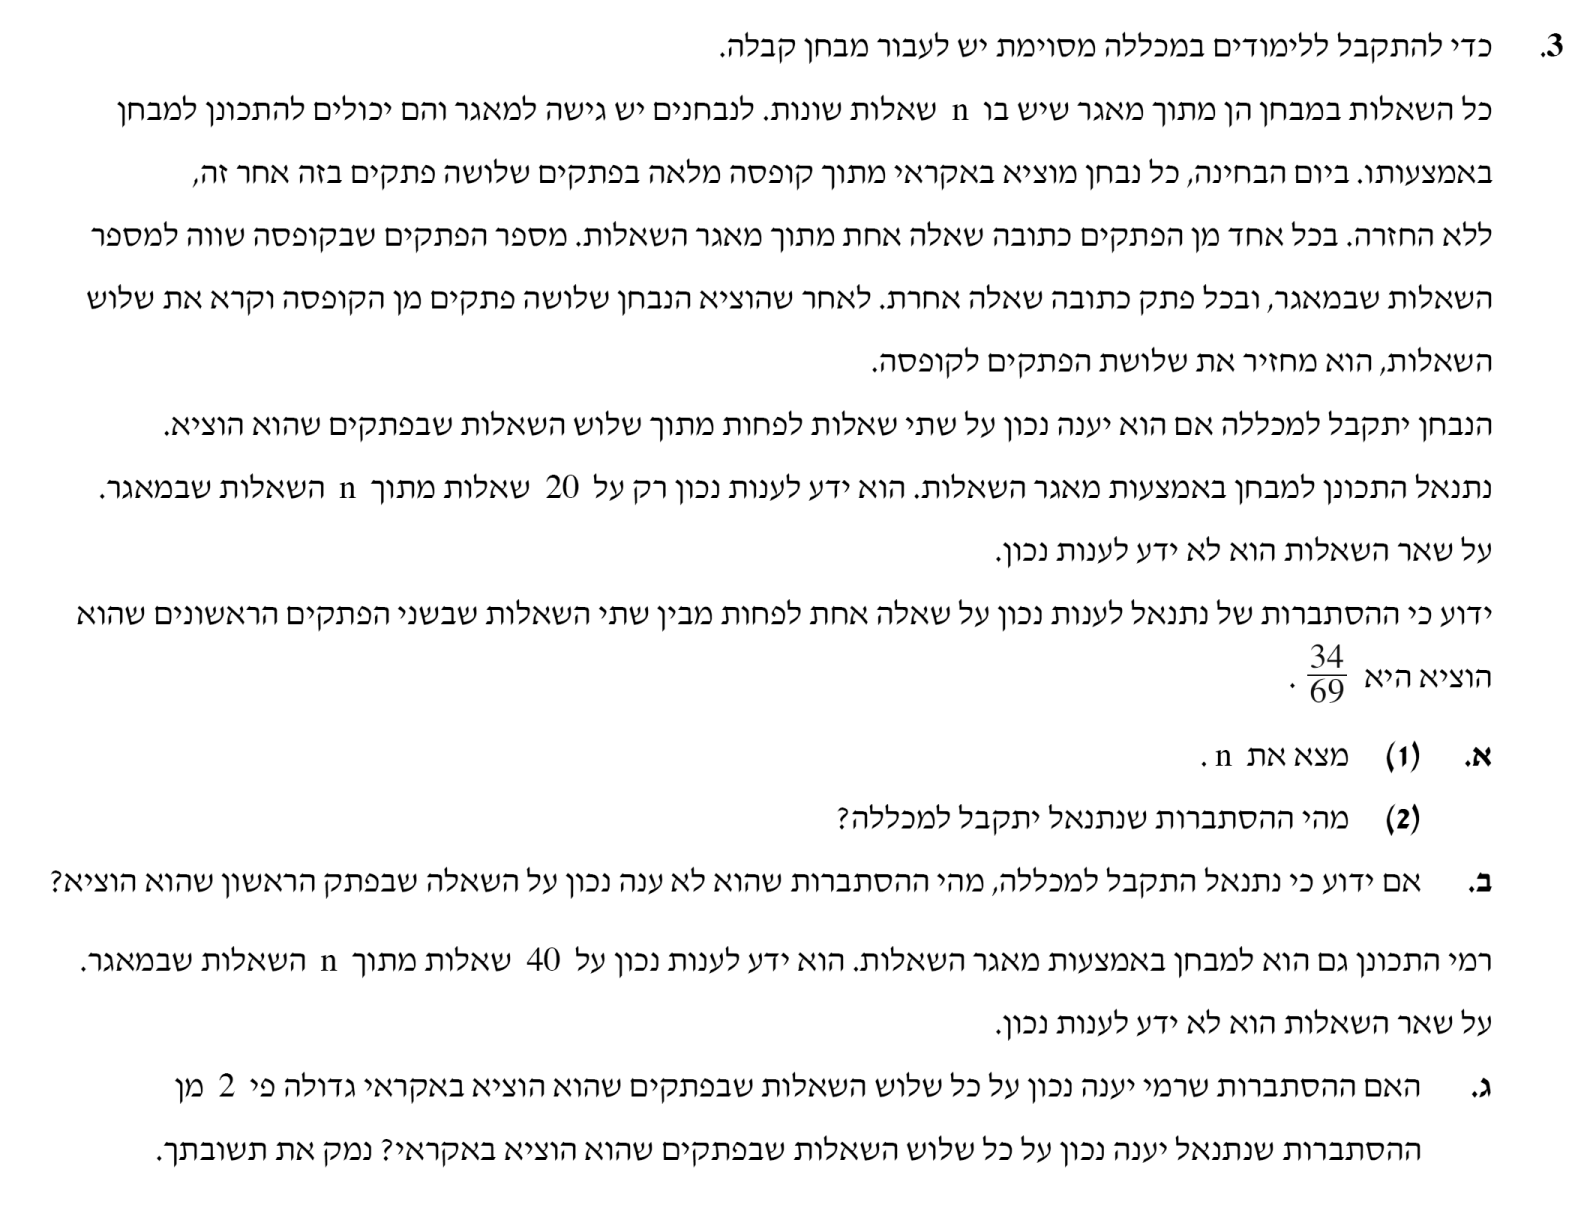
\includegraphics[width=\textwidth]{winter-2022nv-3}
\end{center}

לדעתי ניסוח השאלה ארוכה מדי!

"ידוע כי ההסתברות" לא מכוון להסתברות מותנית. בסעיף א 1 שום מאורע לא תלוי במאורע שנתנאל "ענה נכון
$\ldots$",
אלא פשוט נתונה ההסתברות של המאורע. לדעתי ניתן לפרש את סעיף א 2 כמבקשת את ההסתברות נתנאל יתקבל למכללה "אם ידוע כי 
$\ldots$".
בבדיקת פתרונות באינטרנט לא מצאתי אף אחד שחשב כמוני.

\textbf{סעיף א 1}

התשובה יחסית פשוטה למצוא אבל החישובים מסובכים ולא האמנתי שייצא מהם משהו. נסמן ב-%
$N$ \L{(nachon)}
את המאורע שנתנאל ענה נכון. "לפחות" מכוון להתפלגות בינומית. נחשב את ההסתברות המשלימה כאשר יש להקפיד שהשליפות הן ללא החזרה:
\begin{eqn}
P(N\geq 1)&=&1-\frac{n-20}{n}\cdot\frac{n-20}{n-1}=
\frac{34}{69}\\
\frac{40n-420}{n^2-n}&=&\frac{34}{69}\\
17n^2-1397n+14490&=&0\\
n&=&\frac{1397\pm 983}{34}=70,\, 20.3\,.
\end{eqn}
מספר השאלות הוא מספר שלם ולכן התשובה היא
$70$.

\textbf{סעיף א 2}

כדי להתקבל למכללה נתנאל חייב לענות נכון על שאלות: (א) 
$1,2,3$
או (ב)
$1,2$
או (ג)
$1,3$
או (ד)
$2,3$.

נסמן ב-%
$Y$ \L{(yitkabel)}
את המאורע שהוא יתקבל למכללה. ההסתברות המבוקשת היא:
\begin{eqn}
P(Y)&=&
\frac{20}{70}\cdot\frac{19}{69}+
\frac{20}{70}\cdot\frac{50}{69}\cdot\frac{19}{68}+
\frac{50}{70}\cdot\frac{20}{69}\cdot\frac{19}{68}\\[8pt]
&=&\frac{20\cdot 19\cdot (68+50+50)}{70\cdot 69\cdot 68}=
\frac{76}{391}=0.1944\,.
\end{eqn}
ויתרתי על החישוב של ההסתברות של מאורע (א) כי הוא כלול במאורע (ב). אם מתעקשים אפשר לחשב:
\[
\frac{20}{70}\cdot\frac{19}{69}\cdot\frac{18}{68} + \frac{20}{70}\cdot\frac{19}{69}\cdot \frac{50}{68}=\frac{20}{70}\cdot\frac{19}{69}=\frac{20}{70}\cdot\frac{19}{69}\left(\frac{18}{68}+\frac{50}{68}\right)=\frac{20}{70}\cdot\frac{19}{69}\,.
\]

\textbf{סעיף ב}

ההסתברות המבוקשת היא:
\[
P(\overline{N}/Y)=\frac{P(\overline{N}\cap Y)}{P(Y)}\,.
\]
$P(\overline{N}\cap Y)$
היא הגורם השלישי בחישוב של 
$P(Y)$
בסעיף הקודם ו-%
$P(Y)$
היא התשובה מהסעיף הקודם, לכן:
\begin{eqn}
P(\overline{N}\cap Y)&=&
\frac{\disfrac{50}{70}\cdot\disfrac{20}{69}\cdot\disfrac{19}{68}}
{\disfrac{76}{391}}=\frac{50\cdot 20\cdot 19\cdot 191}{76\cdot 70\cdot 69\cdot 68}=\frac{25}{84}=0.2976\,.
\end{eqn}
בצימצום השבר אפשר להשתמש בפירוקים
$76=4\cdot 19$
ו-%
$391=17\cdot 23$.

\textbf{סעיף ג}

נסמן ב-%
$T=3$ \L{(neTanel)}
את המאורע שנתנאל ענה נכון על שלושת השאלות ונסמן ב-%
$R=3$ \L{(Rami)}
את המאורע שרמי ענה נכון על שלושת השאלות. נשווה את ההסתברויות:
\begin{eqn}
P(R=3)&\stackrel{?}{=}&2P(T=3)\\[8pt]
\frac{40}{70}\cdot\frac{39}{69}\cdot\frac{38}{68}
&\stackrel{?}{=}&
2\cdot\frac{20}{70}\cdot\frac{19}{69}\cdot\frac{18}{68}\\[8pt]
39 &\neq& 9\,,
\end{eqn}
והתשובה היא לא.

% !TeX root = probability.tex

%%%%%%%%%%%%%%%%%%%%%%%%%%%%%%%%%%%%%%%%%%%%%%%%%%%%%%%%%%%%%%

\section{קיץ תשפ"א מועד ב}

\begin{center}
\selectlanguage{english}
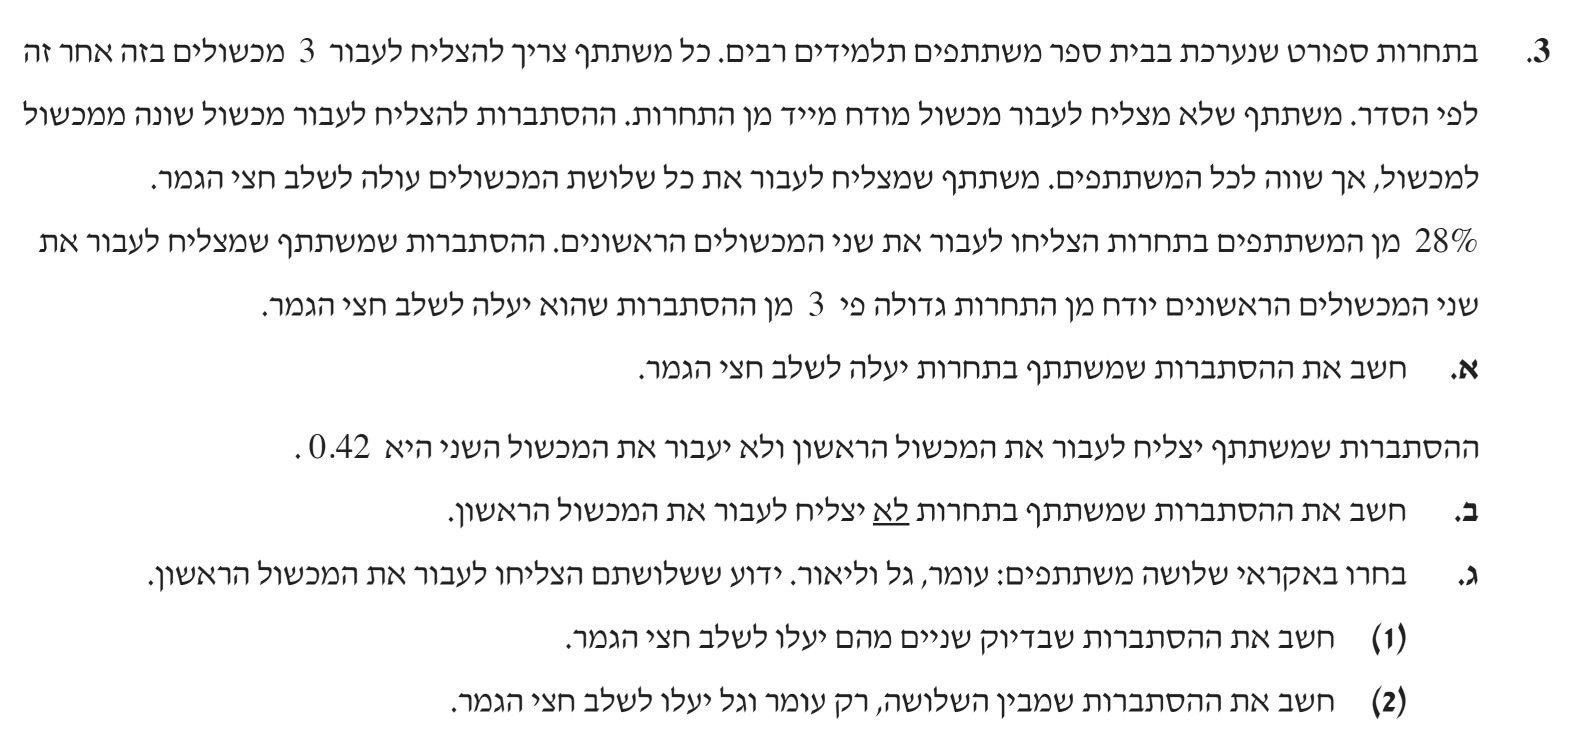
\includegraphics[width=\textwidth]{summer-2021b-3}
\end{center}

נניח שההסתברויות לעבור כל מכשול בלתי-תלויות. נסמן ב-%
$M1, M2, M3$ \L{(mikhshol)}
את המאורעות של לעבור כל מכשול, ונסמן ב-%
$HG$ \L{(hatzi gmar)}
את המאורע לעלות לחצי הגמר.

\textbf{סעיף א}

לפי ההנחה שהצלחה לעבור מכשול בלתי תלוי במכשולים האחרים, ההסתברות לעבור סדרה של מכשולים היא המכפלה של ההסתברויות של המכשולים. נתון ש-%
$P(M1)P(M2)=0.28$.
אם משתתף עבר את שני המכשולים הראשונים, ההסתברות שהוא יעלה לחצי הגמר שווה להתסתברות שהוא יעבור את המכשול השלישי:
\begin{eqn}
P(M3)&=&3(1-P(M3))\\
P(M3)&=&0.25\\
P(HG)&=&P(M1)P(M2)P(M3)=0.28\cdot 0.25=0.07\,.
\end{eqn}

\textbf{סעיף ב}

נתון
$P(M1)P(\overline{M2})=0.42$
ולפי הסתברות שלמה:
\begin{eqn}
P(M1)&=&P(M1)P(M2)+P(M1)P(\overline{M2})=0.28+0.42=0.70\\
P(\overline{M1})&=&1-P(M1)=0.30\,.
\end{eqn}

\textbf{סעיף ג 1}

ההסתברות של משתתף אחד לעלות לחצי הגמר היא:
\[
P(HG/M1)=\frac{P(HG\cap M1)}{P(M1)}=\frac{P(HG)}{P(M1)}=
\frac{0.07}{0.70}=0.01\,,
\]
כאשר אנו משתמשים ב-%
$HG \subseteq M1$
כי משתתף עולה לחצי הגמר רק אם הוא עבר את כל המכשולים, קל וחומר  את המכשול הראשון.

המילה "בדיוק" מכוונת לנוסחת ברנולי, לכן ההסתברות המבוקשת היא:
\[
{3\choose 2}\left(0.01\right)^2\left(0.90\right)^1=0.027\,.
\]

\textbf{סעיף ג 2}

נסמן ב-%
$O,G,L$
את המאורעות שעומר, גל וליאור יעלו לחצי הגמר. נניח כרגיל שההצלחות של המשתתפים בלתי-תלויות:
\[
P(O)P(G)P(\overline{L}) =
\left(0.10\right)\left(0.90\right)\left(0.10\right)=0.009\,.
\]

%%%%%%%%%%%%%%%%%%%%%%%%%%%%%%%%%%%%%%%%%%%%%%%%%%%%%%%%%%%%%

\newpage

\section{קיץ תשפ"א מועד א}

\begin{center}
\selectlanguage{english}
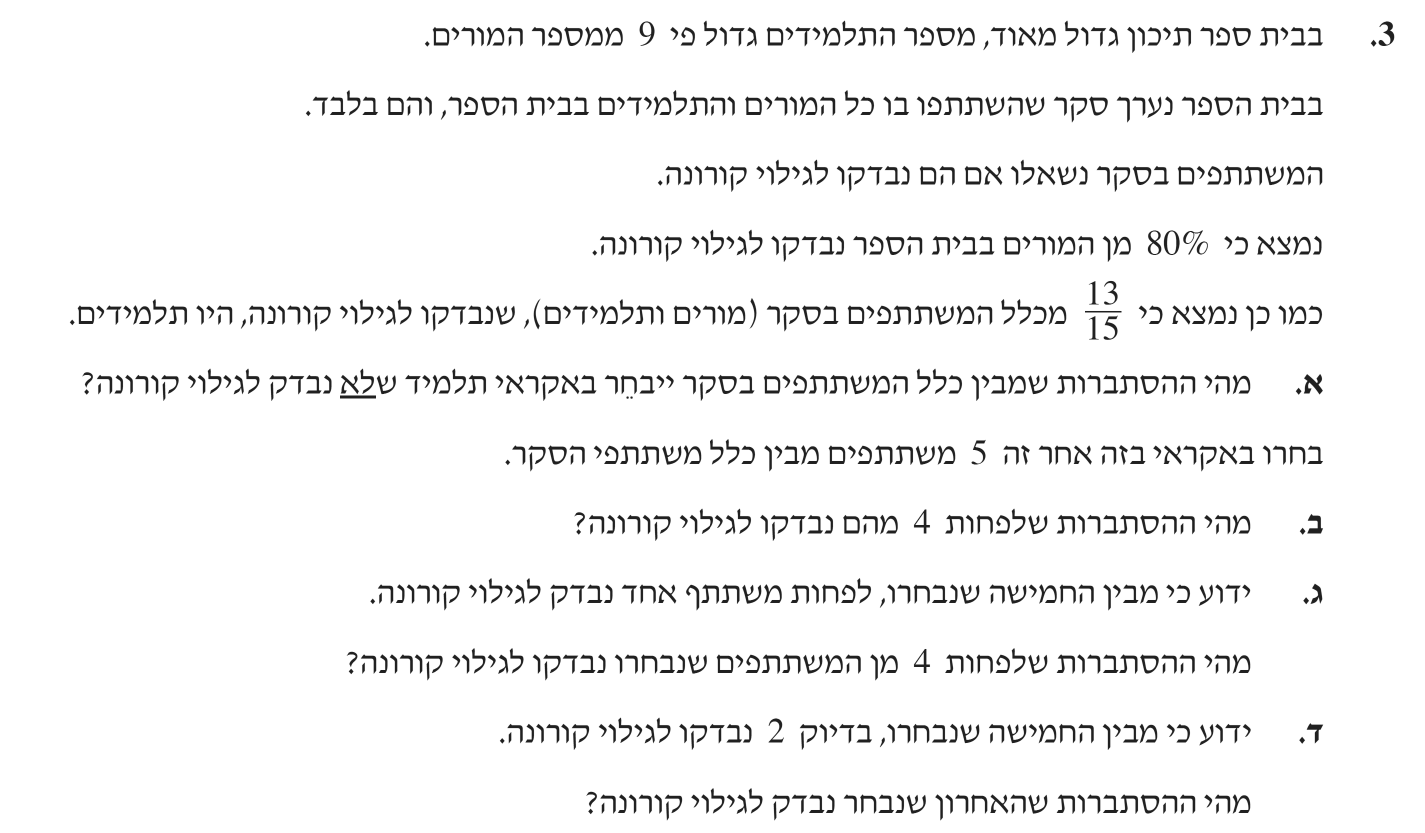
\includegraphics[width=\textwidth]{summer-2021a-3}
\end{center}

הפסקאות "מן המורים" ו-"מכלל המשתתפים" אינן מכוונות להסתברות מותנית, כי הן מתייחסות לכל הקבוצה של המורים וכל הקבוצה של המשתתפים. הפסיק ב-"מכלל המשתתפים (מורים ותלמידים), שנבדקו לגילוי קורונה" מבלבל כי אפשר לפרש שהנתון הוא
$13/15$
"מכלל המשתתפים בסקר".

נסמן ב-%
$M$ \L{(moreh)}
את המאורע של מורה שנסקר בסקר, ואז
$\overline{M}$
הוא המאורע של תלמיד שנסקר בסקר. נסמן ב-%
$N$ \L{(nivdak)}
את המאורע של נבדק לקורונה.

\textbf{סעיף א}

יש שני סוגים של מאורעות ולכן הארגן את המידע בטבלה. 

תחילה נחשב:
\begin{eqn}
P(\overline{M})&=&1-P(M)=9P(M)\\
P(M)&=&0.10\,.
\end{eqn}
נתון ש:
\[
P(N/M)=\frac{P(N\cap M)}{P(M)}=0.80\,,
\]
ולכן:
\[
P(N\cap M) = 0.80P(M)=0.08\,.
\]
את התוצאות הללו נכניס לתאים בטבלה תוך הוספת הסתברויות משלימות:
\begin{center}
\begin{tikzpicture}[scale=1.25]
\draw (0,0) grid[xstep=1.5] (4.5,3);
\node at (3.75,3.3) {$N$};
\node at (2.25,3.3) {$\overline{N}$};
\node at (5,2.5) {$M$};
\node at (5,1.5) {$\overline{M}$};

\node at (3.75,2.5) {$0.08$};
\node at (2.25,2.5) {$0.02$};
\node at (0.75,2.5) {$0.10$};

\node at (3.75,1.5) {$$};
\node at (2.25,1.5) {$$};
\node at (0.75,1.5) {$0.90$};

\node at (0.75,0.5) {$1.0$};
\node at (2.25,0.5) {$$};
\node at (3.75,0.5) {$$};
\end{tikzpicture}
\end{center}
נתון נוסף הוא:
\[
P(\overline{M}/N)=\frac{P(\overline{M}\cap N)}{P(N)}=\frac{13}{15}\,.
\]
נשתמש בהסתברויות משלימות ונקבל:
\begin{eqn}
P(N)&=&P(M\cap N)+P(\overline{M}\cap N)\\[6pt]
&=&0.08+\frac{13}{15}P(N)\\
P(N)&=&0.60\,.
\end{eqn}
נמלא את שאר התאים בטבלה ונמצא את התשובה:
\[
P(\overline{M}\cap \overline{N})=0.38\,.
\]
\begin{center}
\begin{tikzpicture}[scale=1.25]
\draw (0,0) grid[xstep=1.5] (4.5,3);
\node at (3.75,3.3) {$N$};
\node at (2.25,3.3) {$\overline{N}$};
\node at (5,2.5) {$M$};
\node at (5,1.5) {$\overline{M}$};

\node at (3.75,2.5) {$0.08$};
\node at (2.25,2.5) {$0.02$};
\node at (0.75,2.5) {$0.10$};

\node at (3.75,1.5) {$0.52$};
\node at (2.25,1.5) {$0.38$};
\node at (0.75,1.5) {$0.90$};

\node at (0.75,0.5) {$1.0$};
\node at (2.25,0.5) {$0.40$};
\node at (3.75,0.5) {$0.60$};
\end{tikzpicture}
\end{center}

\textbf{סעיף ב}

הניסוח "בזה אחר זה" מכוון להתפלגות בינומית. נקצר את הסימון 
$P(N)$
ל-%
$p$
ולפי סעיף א 
$p=0.60$.
לפחות ארבעה משתתפים שקול לארבעה או חמישה משתתפים:
\begin{eqn}
P(N\geq 4) &=& {5 \choose 4}p^4(1-p)^1+{5 \choose 5}p^5(1-p)^0\\
&=& 5\cdot 0.60^4\cdot 0.40 + 0.60^5=0.3370\,.
\end{eqn}

\textbf{סעיף ג}

המילה "ידוע" מכוון להסתברות מותנית. ברור ש-%
$N\geq 4\subseteq N\geq 1$
ולכן:
\begin{eqn}
P(N\geq 4 / N\geq 1)&=&\frac{P((N\geq 4) \cap (N\geq 1))}{P(N\geq 1)}=\frac{P(N\geq 4)}{P(N\geq 1)}=\frac{P(N\geq 4)}{1-P(N=0)}\\[6pt]
&=& \frac{0.3370}{1-(1-p)^5}=\frac{0.3370}{0.9898}=0.3404\,.
\end{eqn}

\textbf{סעיף ד}

עלינו לחשב את ההסתברות של המאורע: בדיוק אחד מתוך ארבעה המשתתפים הראשונים שנבחרו נבדקו וגם שהמשתתף האחרון שנבחר נבדק. נסמן מאורע זה ב-%
$N_{4A}$,
ונשים לב ש-%
$N_{4A}\subseteq (N=2)$
כי לפי ההגדרה
$N_{4A}$
היא דרך אחת לקבל בדיוק שני נצחונות. "ידוע" מכוון להסתברות מותנית:
\begin{eqn}
P(N_{4A} / (N= 2))&=& \frac{P(N_{4A} \cap (N=2))}{P(N=2)}= \frac{P(N_{4A})}{P(N=2)}\\[10pt]
&=&\frac{{4\choose 1}p^1(1-p)^3\cdot p}{{5\choose 2}p^2(1-p)^2}=\frac{4}{10}\,.
\end{eqn}

%%%%%%%%%%%%%%%%%%%%%%%%%%%%%%%%%%%%%%%%%%%%%%%%%%%%%%%%%%%%%

\newpage

\section{קיץ תשפ"א מועד מיוחד}

\begin{center}
\selectlanguage{english}
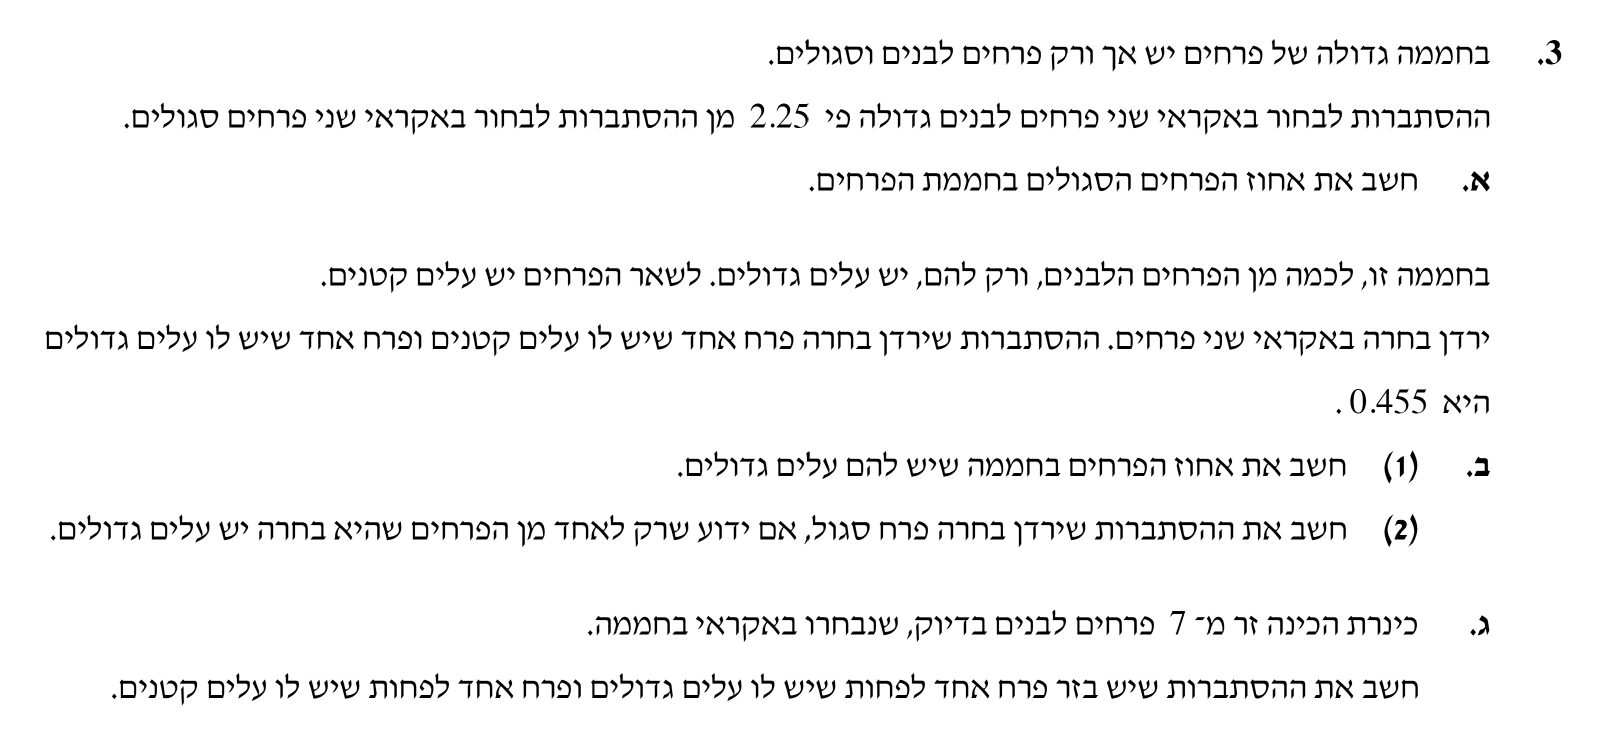
\includegraphics[width=.9\textwidth]{summer-2021sp-3}
\end{center}

\textbf{סעיף א}

נמסן ב-%
$L$ \L{(lavan)}
את המאורע של פרח לבן וב-%
$S$ \L{(segol)}
את המאורע של פרח סגול. מהנתון ניתן לחשב את ההסתברות המבוקשת:
\begin{eqn}
P(L=2)&=&\frac{9}{4}P(S=2)\\[6pt]
(1-P(S))^2&=&\left(\frac{3}{2}P(S)\right)^2\\[6pt]
P(S)&=&\frac{2}{5}=40\%\,,
\end{eqn}
כאשר השתמשנו בהנחה שהבחירות של שני פרחים בלתי תלויות ובעובדה שהסתברויות משלימות.

\textbf{סעיף ב}

נסמן ב-%
$G$ \L{(gadol)}
את המאורע של עלים גדולים.

הסתבכתי בשאולה זו כי ניסיתי לחשב 
$P(G/L)$
בלי לשים לב שאין כאן הסתברות מותנית, כי המידע שפרח הוא לבן לא תורם  מידע אם לפרח עלים גדולים. הפתרון פשוט מתקבל על ידי חישוב ההסתברות 
$P(G)$
וההסתברות המשלימה. עם המידע הנתון על הבחירות של ירדן, ההסתברות המבוקשת היא:
\begin{eqn}
P(G\overline{G})&=&{2\choose 1}P(G)^1(1-P(G))^1=0.455\\
2P(G)^2 - 2P(G) + 0.455&=&0\\
P(G)&=&\frac{2\pm\sqrt{0.36}}{4}=\frac{1\pm\frac{3}{10}}{2}\\
&=&\frac{7}{20},\,\frac{13}{20}=0.35\,,0.65\,.
\end{eqn}
אבל אחוז הפרחים עם עלים גדולים לא יכול להיות גבוה יותר ממספר הפרחים הלבנים
$0.6$,
ולכן
$P(G)=0.35=35\%$.

\textbf{סעיף ג 1}

נסמן ב-%
$1G$
את המאורע שרק לאחד הפרחים מתוך שניים יש עלים גדולים. נתון ש-%
$P(1G)=0.455$.
החישוב יהיה קל יותר אם נשים לב ש-%
$0.455=0.35\cdot 1.3=\frac{7}{20}\cdot \frac{13}{10}$.
המילה "ידוע" מכוון להסתברות מותנית:
\begin{eqn}
P(S=1/1G)&=&\frac{P(S=1 \cap 1G)}{P(1G)}=\frac{{2\choose 1}P(S)P(G)}{P(1G)}\\
&=&\frac{2\cdot\frac{4}{10}\frac{7}{20}}{\frac{7}{20}\frac{13}{10}}=\frac{8}{13}\,.
\end{eqn}

\textbf{סעיף ג 2}

המשפט בראשון אומר שבוחרים רק מתוך הפרחים הלבנים:
\[
P(G/L)=\frac{P(G\cap L)}{P(L)}=\frac{P(G)}{P(L)}=\frac{7/20}{6/10}=\frac{7}{12}\,.
\]
לפי הסתברות משלימה
$P(\overline{G}/L)=\frac{5}{12}$.
מילים "בדיוק" ו-"לפחות" מכוונות לנוסחת ברנולי. ההסתברות המבוקשת היא ההסתברות המשלימה לאפס פרחים עם עלים גדולים ואפס פרחים עם עלים קטנים:
\[
1-\left(\frac{7}{12}\right)^7-\left(\frac{5}{12}\right)^7=0.9748\,.
\]

%%%%%%%%%%%%%%%%%%%%%%%%%%%%%%%%%%%%%%%%%%%%%%%%%%%%%%%%%

\newpage


\section{חורף תשפ"א}

\begin{center}
\selectlanguage{english}
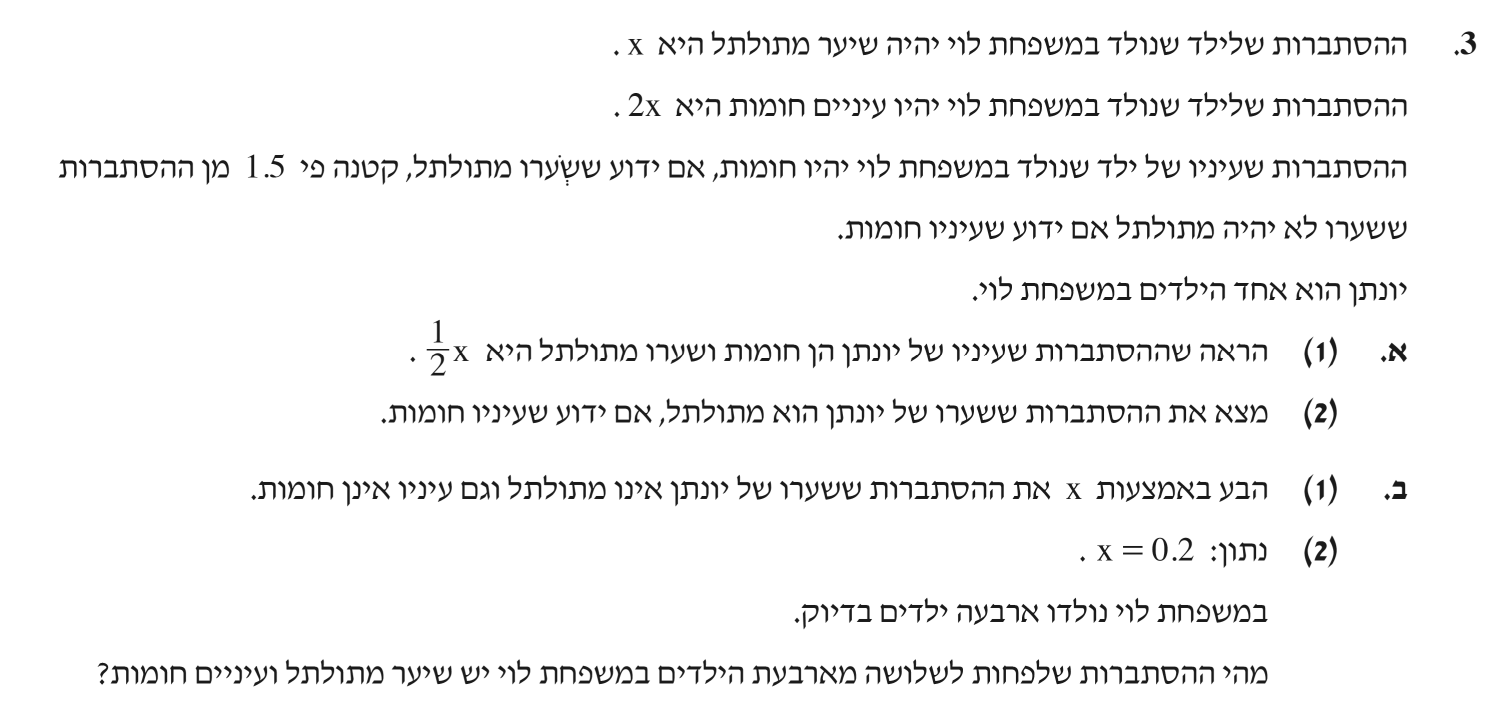
\includegraphics[width=.85\textwidth]{winter-2021-3}
\end{center}

נמסן ב-%
$H$ \L{(hume)}
את המאורע של עיניים חומות ונסמן ב-%
$M$ \L{(metultal)}
את המאורע של שיער מטולטל.

\textbf{סעיף א 1}

בשאלה שני סוגים של מאורעות ולכן נארגן את המידע בטבלה. נתון 
$P(M)=x, P(H)=2x$
וסימנו 
$y=P(H\cap M)$.
\begin{center}
\begin{tikzpicture}[scale=1.25]
\draw (0,0) grid[xstep=1.5] (4.5,3);
\node at (3.75,3.3) {$H$};
\node at (2.25,3.3) {$\overline{H}$};
\node at (5,2.5) {$M$};
\node at (5,1.5) {$\overline{M}$};

\node at (3.75,2.5) {$y$};
\node at (2.25,2.5) {$$};
\node at (0.75,2.5) {$x$};

\node at (3.75,1.5) {$3y$};
\node at (2.25,1.5) {$$};
\node at (0.75,1.5) {$$};

\node at (0.75,0.5) {$$};
\node at (2.25,0.5) {$$};
\node at (3.75,0.5) {$2x$};
\end{tikzpicture}
\end{center}
המילה "ידוע" מכוון להסתברות מותנית ונשתמש ביחס הנתון:
\begin{eqn}
1.5P(H/M)&=&P(\overline{M}/H)\\[4pt]
\frac{1.5P(H\cap M)}{P(M)}&=&\frac{P(\overline{M}\cap H)}{P(H)}\\[4pt]
\frac{1.5y}{x}&=&\frac{P(\overline{M}\cap H)}{2x}\\[4pt]
P(\overline{M}\cap H)&=&3y\,.
\end{eqn}
צירפנו ערך זה לטבלה. מהעמודה
$H$
מתקבל
$y+3y=2x$
ולכן
$P(M\cap H)=y=x/2$.

\textbf{סעיף א 2}

ההסתברות המבוקשת היא:
\[
P(M/H)= \frac{P(M\cap H)}{P(H)}=\frac{x/2}{2x}=\frac{1}{4}\,.
\]

\textbf{סעיף ב 1}

נציב 
$x/2$
עבור 
$y$
ו-%
$P(\overline{H}\cap M)$.
ההסתברות המבוקשת היא עבור התא האמצעי וניתן לחשבה על ידי הסתברות משלימה:
\[
P(\overline{H}\cap \overline{M})=1-\left(\frac{x}{2}+\frac{x}{2}+\frac{3x}{2}\right)=1-\frac{5x}{2}\,.
\]
\begin{center}
\begin{tikzpicture}[scale=1.25]
\draw (0,0) grid[xstep=1.5] (4.5,3);
\node at (3.75,3.3) {$H$};
\node at (2.25,3.3) {$\overline{H}$};
\node at (5,2.5) {$M$};
\node at (5,1.5) {$\overline{M}$};

\node at (3.75,2.5) {$\disfrac{x}{2}$};
\node at (2.25,2.5) {$\disfrac{x}{2}$};
\node at (0.75,2.5) {$x$};

\node at (3.75,1.5) {$\disfrac{3x}{2}$};
\node at (2.25,1.5) {$$};
\node at (0.75,1.5) {$$};

\node at (0.75,0.5) {$$};
\node at (2.25,0.5) {$$};
\node at (3.75,0.5) {$2x$};
\end{tikzpicture}
\end{center}

\textbf{סעיף ב 2}

במילה "לפחות" מכוונת לנוסחת ברנולי. נסמן
$p=P(H\cap M)$
ונחשב:
\begin{eqn}
P(p\geq 3) = P(p=3 \cup p=4)&=& {4\choose 3}p^3(1-p)^1+{4\choose 4}p^4(1-p)^0\\[6pt]
&=&4\cdot 0.0009 + 0.0001 = 0.0037\,.
\end{eqn}

%%%%%%%%%%%%%%%%%%%%%%%%%%%%%%%%%%%%%%%%%%%%%%%%%%%%%%%%%

\newpage

\section{חורף תשפ"א מועד נבצרים}

\begin{center}
\selectlanguage{english}
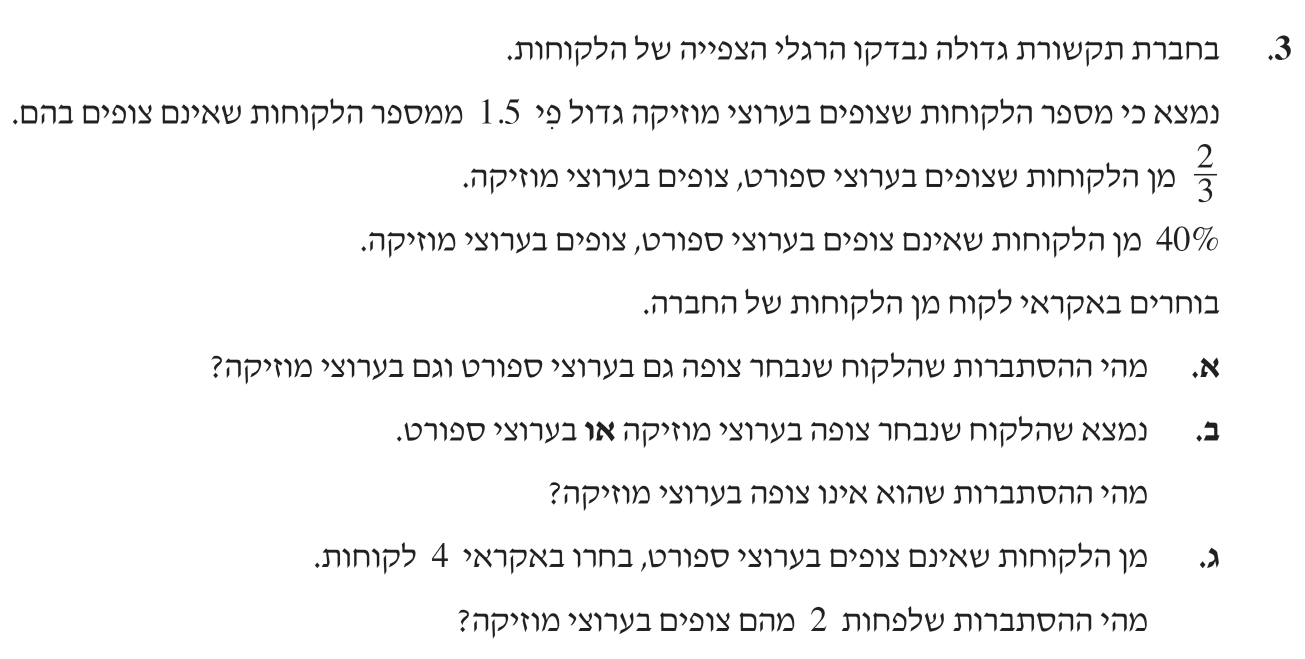
\includegraphics[width=\textwidth]{winter-2021nv-3}
\end{center}

נסמן ב-%
$M$ \L{(muzika)}
את המאורע של צופים במוזיקה ונסמן ב-%
$S$ \L{(sport)}
את המאורע של צופים בספורט. השאלה שואלת על שני סוגים של מאורעות ולכן נארגן את המידע בטבלה.

מהנתון הראשון ניתן לחשב את
$P(M)$:
\begin{eqn}
P(M)&=&1.5P(\overline{M})=1.5 (1-P(M))\\
P(M)&=&3/5\,.
\end{eqn}
בשני המשפטים הבאים, "מן הלקוחות" מכוון להסתברות מותנית:
\begin{eqn}
P(M/S)&=&\frac{P(M\cap S)}{P(S)}=2/3\\[4pt]
P(M\cap S)&=&(2/3)P(S)\\[4pt]
P(M/\overline{S})&=&\frac{(M\cap \overline{S})}{P(\overline{S})}=2/5\\[4pt]
P(M\cap \overline{S})&=&(3/5)P(\overline{S})\,.
\end{eqn}
נשתמש בהסתברות שלמה כדי לחשב את 
$P(S)$:
\begin{eqn}
P(M)&=&P(M\cap S)+P(M\cap \overline{S})=3/5\\
&=&(2/3)P(S)+(2/5)P(\overline{S})=3/5\\
P(S)&=&3/4\,.
\end{eqn}
לאחר שנחשב את
$P(M\cap S)$
ו-%
$P(M\cap \overline{S})$
מ-%
$P(S)$,
נוכל למלא אתת הטבלה:
\begin{center}
\begin{tikzpicture}[scale=1.25]
\draw (0,0) grid[xstep=1.5] (4.5,3);
\node at (3.75,3.3) {$M$};
\node at (2.25,3.3) {$\overline{M}$};
\node at (5,2.5) {$S$};
\node at (5,1.5) {$\overline{S}$};

\node at (3.75,2.5) {$\disfrac{1}{2}$};
\node at (2.25,2.5) {$\disfrac{1}{4}$};
\node at (0.75,2.5) {$\disfrac{3}{4}$};

\node at (3.75,1.5) {$\disfrac{1}{10}$};
\node at (2.25,1.5) {$\disfrac{3}{20}$};
\node at (0.75,1.5) {$\disfrac{1}{4}$};

\node at (0.75,0.5) {$1$};
\node at (2.25,0.5) {$\disfrac{2}{5}$};
\node at (3.75,0.5) {$\disfrac{3}{5}$};
\end{tikzpicture}
\end{center}

\textbf{סעיף א}

התשובה נמצאת בתא 
$P(M\cap S)=1/2$.

\textbf{סעיף ב}

המילא "או" מכוון לאיחוד של שני מאורעות. בעזרת תרשים
\L{Venn}
נקבל:
\[
P(M\cup S)=P(M)+P(S)-P(M\cap S)=\frac{3}{5}+\frac{3}{4}-\frac{1}{2}=\frac{17}{20}\,.
\]
ההמשך בהסתברות מותנית. הניסוח לא שגרתי אבל לא קשה: "נמצא שלקוח שנבחר ... מה ההסתברות 
\textbf{שהוא}":
\[
P(\overline{M}/M\cup S)=\frac{P(\overline{M}\cap (M\cup S))}{P(M\cup S)}=\frac{P(S\cap \overline{M})}{P(M\cup S)}=\frac{1/4}{17/20}=5/17\,.
\]
ברור ש-%
$M\cap\overline{M}$
היא הקבוצה הריקה ולכן
$\overline{M}\cap (M\cup S))=S\cap \overline{M}$.

\textbf{סעיף ג}

מהמידע בטבלה נחשב את ההסתברות שלבחור לקוח אחד כנדרש:
\begin{eqn}
P(M/\overline{S})&=&\frac{P(M\cap\overline{S})}{P(S)}=\frac{1/10}{3/4}=\frac{2}{5}\,.
\end{eqn}
"לפחות שניים" מכוון להתפלגות בינום, ונעדיף לחשב את ההסתברות המשלימה:
\begin{eqn}
P(M/\overline{S}\geq 2)&=&1-P(M/\overline{S}<2)\\[6pt]
&=&1-{4\choose 0}\left(\frac{2}{5}\right)^0\left(\frac{3}{5}\right)^4-{4\choose 1}\left(\frac{2}{5}\right)^1\left(\frac{3}{5}\right)^3\\
&=&\frac{328}{625}=0.5248\,.
\end{eqn}

%%%%%%%%%%%%%%%%%%%%%%%%%%%%%%%%%%%%%%%%%%%%%%%%%%%%%%%%%

\newpage

\section{חורף תשפ"א מועד מאוחר}

\begin{center}
\selectlanguage{english}
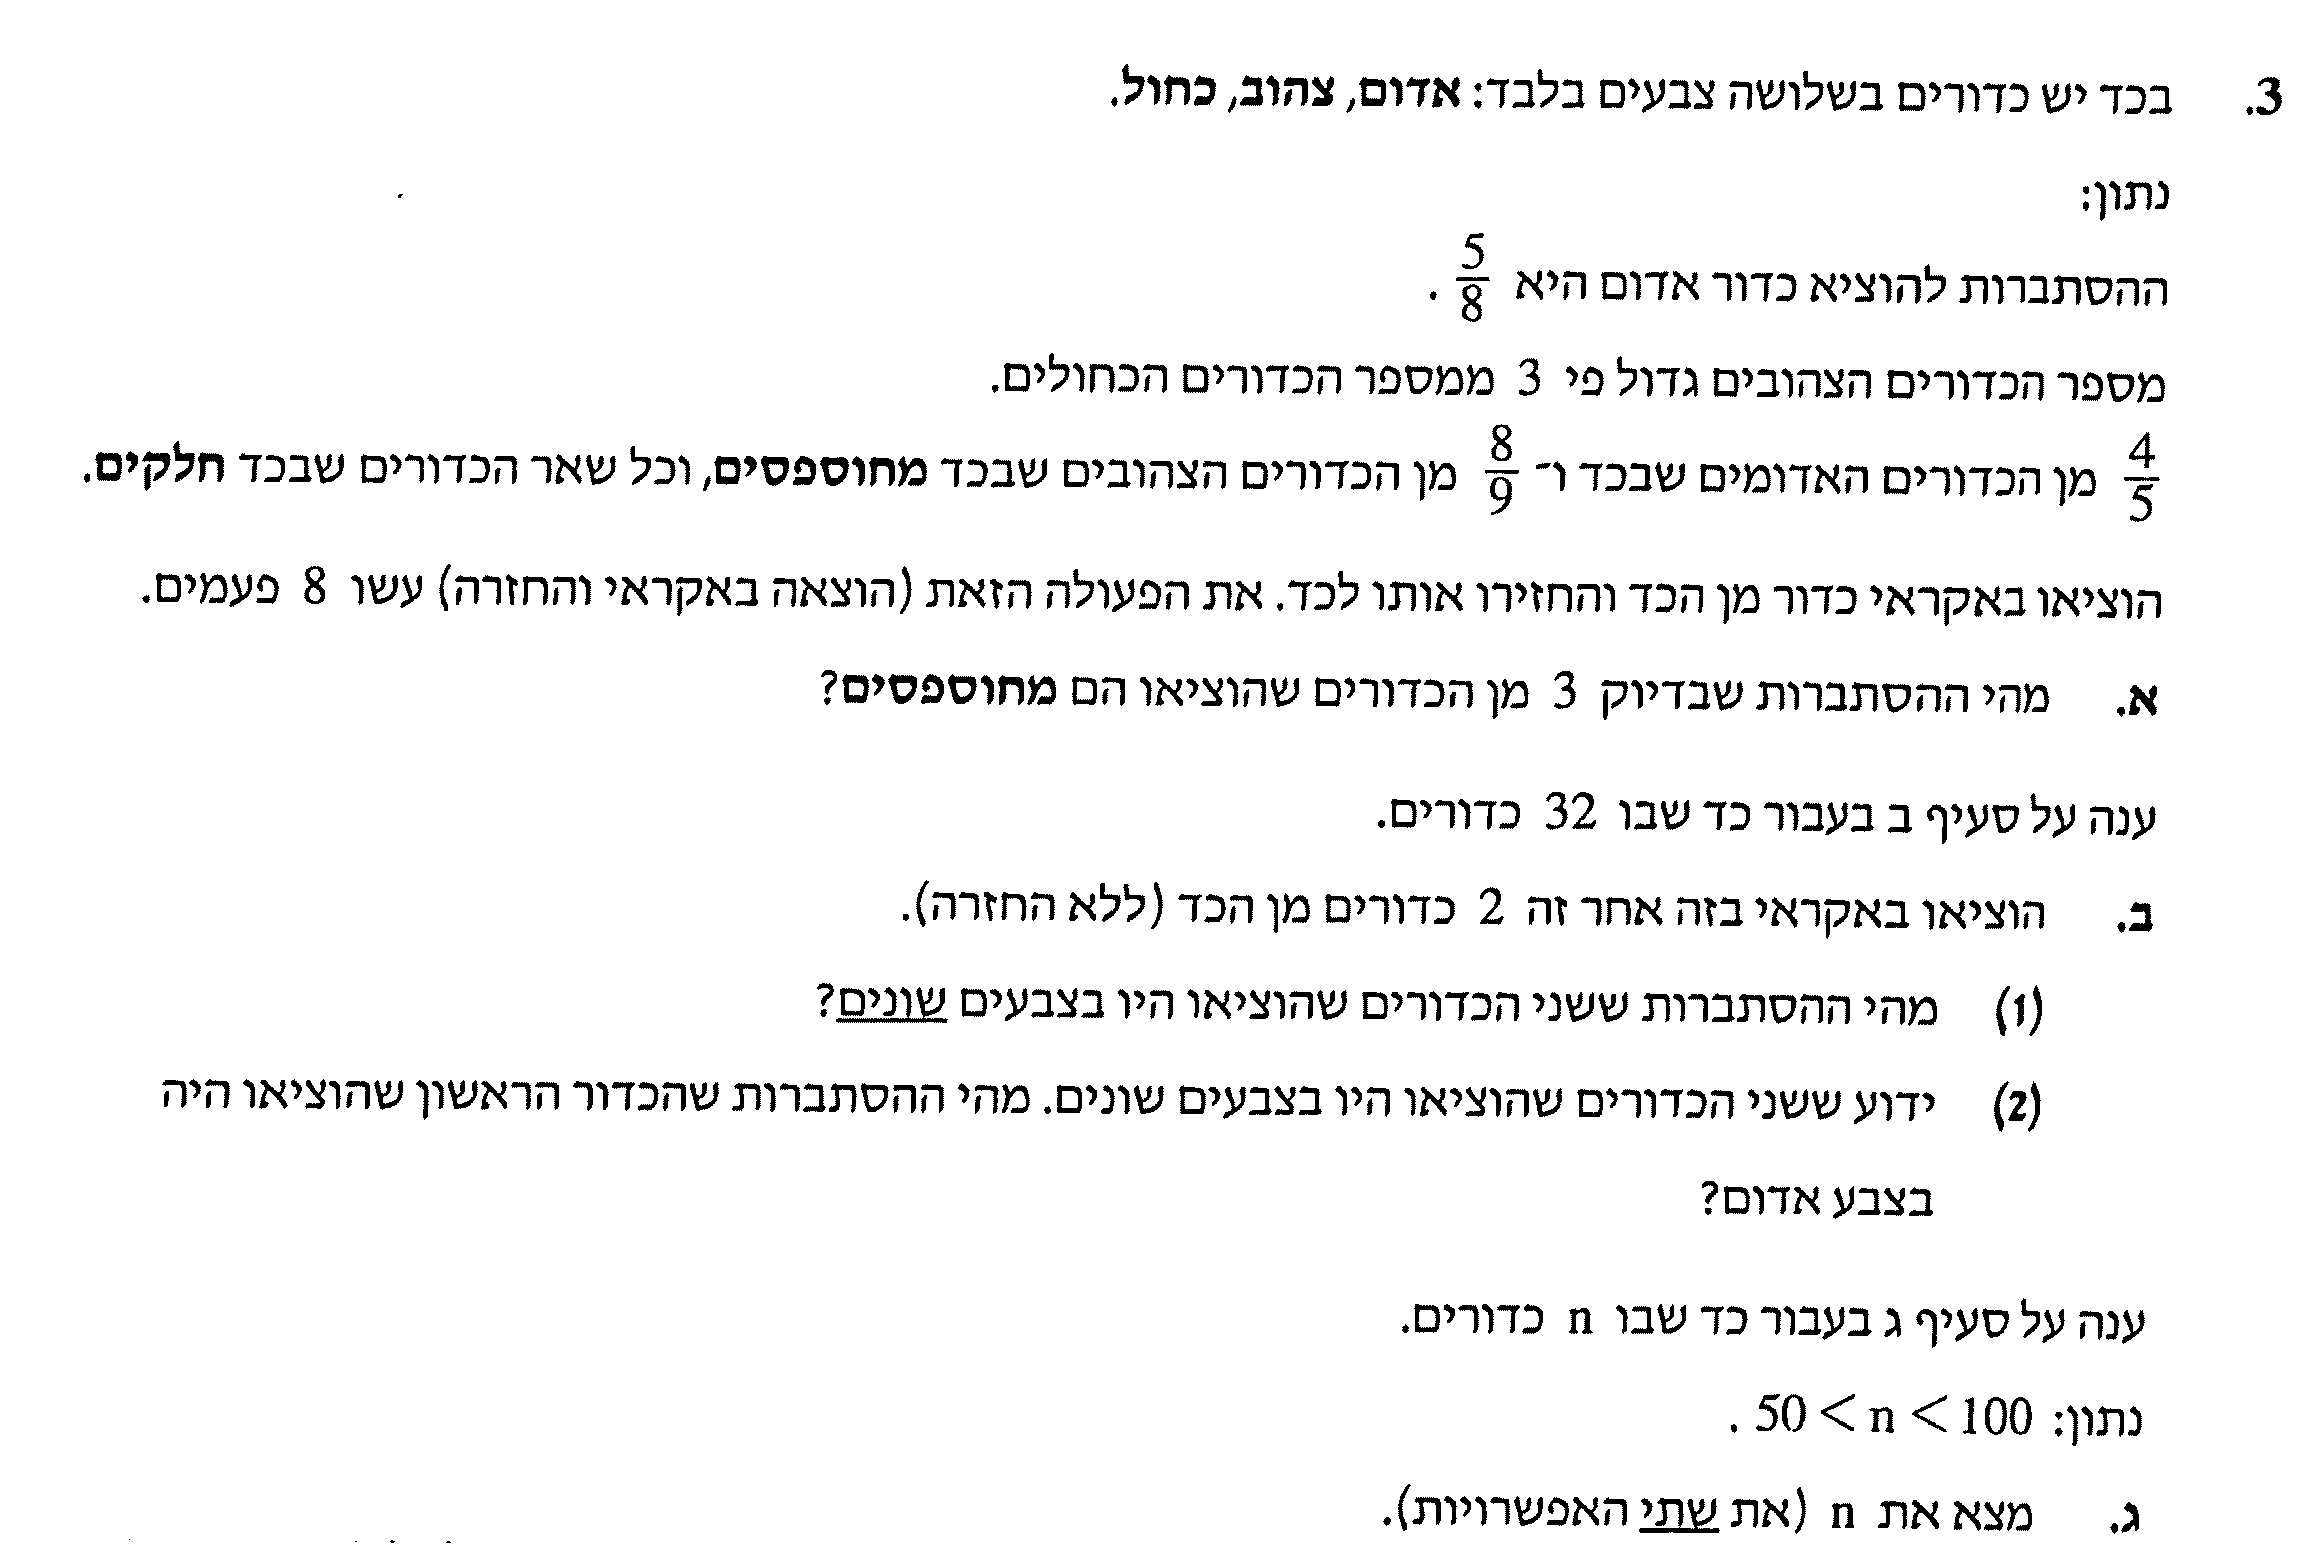
\includegraphics[width=\textwidth]{winter-2021lt-3}
\end{center}

נסמן ב-%
$A$ \L{(adom)}, $T$ \L{(tzahov)}, $K$ \L{(kakhol)}
את המאורעות של הוצאת כדורים אדומים, צהובים וכחולים, בהתאמה. נתון
$P(A)=5/8$, $3P(T)=P(K)$.
נסמן
$x=P(K)$
ונסכם הסתברויות כדי לקבל את המשוואה
\[
5/8+3x+x=1\,,
\]
שפתרונה הוא
$x=3/32$.
נארגן את המידע בטבלה.
\begin{center}
\selectlanguage{english}
\begin{tikzpicture}[scale=1.25]
\draw (0,0) grid[xstep=1.2cm] (4.8,3);
\node at (4.2,3.3) {$A$};
\node at (3,3.3) {$T$};
\node at (1.8,3.3) {$K$};
\node at (5.3,2.5) {$M$};
\node at (5.3,1.5) {$\overline{M}$};

\node at (4.2,2.5) {$$};
\node at (3,2.5) {$$};
\node at (1.8,2.5) {$$};
\node at (0.6,2.5) {$$};

\node at (4.2,1.5) {$$};
\node at (3,1.5) {$$};
\node at (1.8,1.5) {$$};
\node at (0.6,1.5) {$$};

\node at (4.2,0.5) {$5/8$};
\node at (3,0.5) {$9/32$};
\node at (1.8,0.5) {$3/32$};
\node at (0.6,0.5) {$1$};
\end{tikzpicture}
\end{center}
נסמן ב-%
$M$ \L{(mekhuspas)}
את האירוע של כדור מחוספס. נתון:
\begin{eqn}
P(M\cap A)&=&\frac{4}{5}\,P(A)=\frac{1}{2}\\[6pt]
P(M\cap T)&=&\frac{8}{9}\,P(T)=\frac{1}{4}\,.
\end{eqn}
תחילה נראה לי שחסר נתון כדי להמשיך עד שקראתי בעיון את השאלה. הפסקה "כל שאר הכדורים חלקים" אומר ש-%
$P(M\cap K)=0$
וניתן למלא את כל התאים בטבלה עם הסתברויות משלימות:
\begin{center}
\selectlanguage{english}
\begin{tikzpicture}[scale=1.25]
\draw (0,0) grid[xstep=1.2cm] (4.8,3);
\node at (4.2,3.3) {$A$};
\node at (3,3.3) {$T$};
\node at (1.8,3.3) {$K$};
\node at (5.3,2.5) {$M$};
\node at (5.3,1.5) {$\overline{M}$};

\node at (4.2,2.5) {$1/2$};
\node at (3,2.5) {$1/4$};
\node at (1.8,2.5) {$0$};
\node at (0.6,2.5) {$3/4$};

\node at (4.2,1.5) {$1/8$};
\node at (3,1.5) {$1/32$};
\node at (1.8,1.5) {$3/32$};
\node at (0.6,1.5) {$1/4$};

\node at (4.2,0.5) {$5/8$};
\node at (3,0.5) {$9/32$};
\node at (1.8,0.5) {$3/32$};
\node at (0.6,0.5) {$1$};
\end{tikzpicture}
\end{center}

\textbf{סעיף א}

"בדיוק" מכוון לנוסחת ברנולי. ההסתברות היא:
\[
P(M=3)={8\choose 3}\left(\frac{3}{4}\right)^3
\left(\frac{1}{4}\right)^5=56\cdot\frac{27}{65536}=\frac{189}{8192}=0.0231\,.
\]

\textbf{סעיף ב 1}

השליפות הן אחת אחרי השנייה ולכן נארגן את המידע בעץ, כאשר בכל שלב אפשר לשלוף כדור בצבע מסויים. השליפה היא ללא החזרה ולכן ההסתברויות שונות בשליפה הראשונה והשנייה.
\begin{center}
\begin{tikzpicture}
[grow=right,
level 1/.append style={level distance=3cm,
                       sibling distance=6.5em},
level 2/.append style={level distance=5cm,
                       sibling distance=2em}]
\node[left] {} % root
child {
  node[right] {$\scriptstyle K$}
    child {
      node[right] {}
      edge from parent node[below] {$\scriptstyle 2/31$}
    }
    child {
      node[right] {$\scriptstyle KT=TK$}
      edge from parent node[below,near end] {$\scriptstyle 9/31$}
    }
    child {
      node[right] {$\scriptstyle KA=AK$}
      edge from parent node[above] {$\scriptstyle 20/31$}
    }
    edge from parent node[below,yshift=-2mm] 
     {$\scriptstyle 3/32$}
}
child {
  node[right] {$\scriptstyle T$}
    child {
      node[right] {$\scriptstyle TK$}
      edge from parent node[below] {$\scriptstyle 3/31$}
    }
    child {
      node[right] {}
      edge from parent node[below,near end] {$\scriptstyle 8/31$}
    }
    child {
      node[right] {$\scriptstyle TA=AT$}
      edge from parent node[above] {$\scriptstyle 20/31$}
    }
    edge from parent node[below] {$\scriptstyle 9/32$}
}
child {
  node[right] {$\scriptstyle A$}
    child {
      node[right] {$\scriptstyle AK$}
      edge from parent node[below] {$\scriptstyle 3/31$}
    }
    child {
      node[right] {$\scriptstyle AT$}
      edge from parent node[below,near end] {$\scriptstyle 9/31$}
    }
    child {
      node[right] {}
      edge from parent node[above] {$\scriptstyle 19/31$}
    }
    edge from parent node[above,yshift=2mm,xshift=-4pt]
      {$\scriptstyle 20/32$}
}
;
\end{tikzpicture}
\end{center}
נסמן ב-%
$S$ \L{(shoneh)}
את המאורע שהכדורים בצבעים שונים:
\begin{eqn}
P(S)=P(AT\cup AK \cup TK)&=&
\frac{1}{32\cdot 31}
(2\cdot 20\cdot 9 + 2\cdot 20\cdot 3 + 2\cdot 3\cdot 9))\\[6pt]
&=&\frac{534}{992}=0.5383\,.
\end{eqn}
בדיעבד היה קל יותר לחשב את ההסתברות המשלימה לשליפת שני כדורים מאותו צבע!

\textbf{סעיף ב 2}

נסמן ב-%
$A_1$
את המאורע שהכדור הראשון בצבע אדום. "ידוע" מכוון להסתברות מותנית:
\begin{eqn}
P(A_1/S)&=&\frac{P(A_1\cap S)}{P(S)}=\frac{P(AT\cup AK)}{P(S)}\\[12pt]
&=&
\disfrac{
\disfrac{20\cdot 9 +  20\cdot 3}{32\cdot 31\rule[-5pt]{0pt}{5pt}}
}{
\disfrac{\rule[5pt]{0pt}{5pt}534}{32\cdot 31}
}=\frac{40}{89}=0.4494\,.
\end{eqn}

\textbf{סעיף ג}

$P(K)=3/32$
ולכן מספר הכדורים הכחולים הוא
$3n/32$.
בהנחה הברורה שיש מספר שלם של כדורים כחולים, הערכים ההאפשריים של 
$n$
הם
$32, 64, 96, 128,\ldots$.
בטווח הנתון האפשריויות הם
$64, 96$.
% !TeX root = probability.tex

%%%%%%%%%%%%%%%%%%%%%%%%%%%%%%%%%%%%%%%%%%%%%%%%%%%%%%%%%%%%%%

\section{קיץ תש"פ מועד ב}

\begin{center}
\selectlanguage{english}
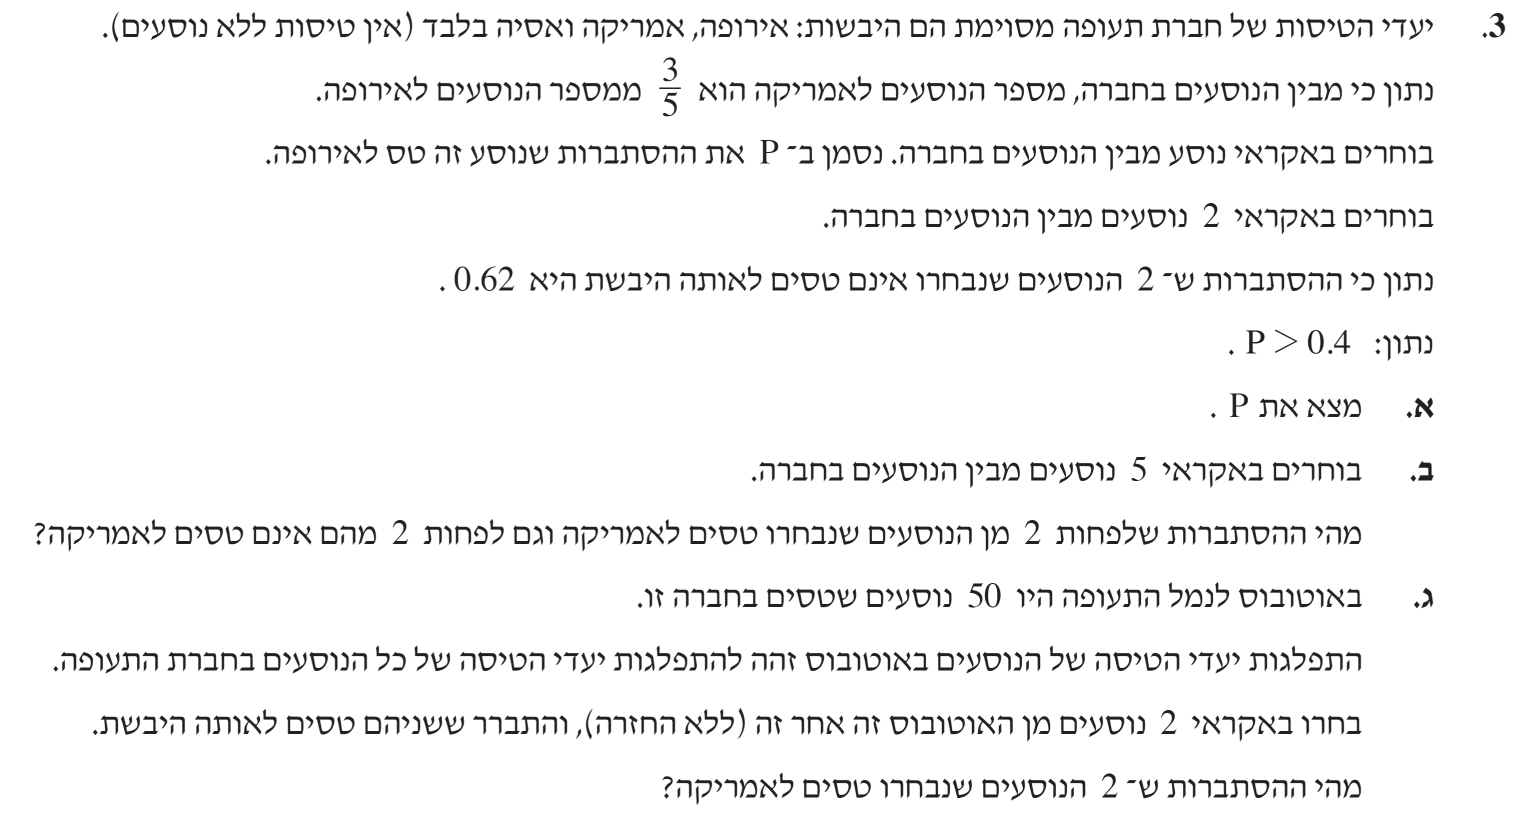
\includegraphics[width=.85\textwidth]{summer-2020b-3}
\end{center}

נסמן את המאורעות:
$AM$ 
עבור טיסה לאמריקה,
$EU$
עבור טיסה לאירופה,
$AS$
עבור טיסה לאסיה. נתון
$P(EU)=p$.\footnote{%
אני מעדיף אות קטנה 
$p$
עבור ההסתברות כי אות גדולה תמיד מסמנת את ההסתברות של מאורע כגון
$P(EU)$.}
לפי המידע הנתון
$P(AM)=\frac{3}{5}p$
ולפי הסתברות משלימה
$P(AS)=1-p-\frac{3}{5}p=1-\frac{8}{5}p$.

\textbf{סעיף א}

נניח שהבחירות של שני הנוסעים של יעדי הטיסות בלתי-תלויות. נתון שההסתברות שבחרו בטיסות שונות היא 
$0.62$.
אפשר לחשב הסתברות זו אבל אפשר גם לחשב את ההסתברות המשלימה
$0.38$
ששניהם בחרו את אותו יעד:
\begin{eqnarray*}
p^2 + \left(\frac{3}{5}p\right)^2+\left(1-\frac{8}{5}p\right)^2&=&0.38\\
p^2 + \frac{9}{25}p^2+1-\frac{16}{5}p+\frac{64}{25}p^2&=&0.38\\
98p^2 -80p+15.5 &=&0\,.
\end{eqnarray*}
נפתור את המשוואה הריבועית ונקבל
$p=\frac{80\pm 18}{196}= 0.5, 0.3$.
השאלה מבקשת הסתברות גדול מ-%
$0.4$
ולכן התשובה היא
$0.5$.

\textbf{סעיף ב}

נסמן את ההסתברות המבוקשת ב-%
$AM22$.
הדרך היחידה שגם לפחות שניים טסים לאמריקה ושניים לא היא ששלושה טסים לשם ושניים לא, או להיפך. ההסתברות לטיסה לאמריקה היא
$\frac{3}{5}p=0.3$.
לפי חוק ברנולי:
\[
P(AM22)={5 \choose 2}(0.3)^2(0.7)^3 +{5 \choose 2}(0.7)^2(0.3)^3=
(10\cdot 0.09 \cdot 0.49) (0.7+0.3)=0.441\,.
\]

\begin{center}
\begin{tikzpicture}
[grow=right,
level 1/.append style={level distance=4cm,
                       sibling distance=7em},
level 2/.append style={level distance=4cm,
                       sibling distance=2.5em}]
\node[left] {$\scriptstyle (15,25,10)$} % root
child {
  node[right] {$\scriptstyle (15,25,9)$}
    child {
      node[right] {$\scriptstyle AS2$}
      edge from parent node[below] {$\scriptstyle 9/49$}
    }
    child {
%      node[right] {$$}
      edge from parent 
        node[below,near end] {$\scriptstyle 25/49$}
    }
    child {
%      node[right] {$$}
      edge from parent node[above] {$\scriptstyle 15/49$}
    }
    edge from
      parent node[below,yshift=-2mm] {$\scriptstyle 10/50$}
      node[above right] {\R{אסיה}}
}
child {
  node[right] {$\scriptstyle (15,24,10)$}
    child {
%      node[right] {$$}
      edge from parent node[below] {$\scriptstyle 10/49$}
    }
    child {
      node[right] {$\scriptstyle EU2$}
      edge from parent 
      node[below,near end] {$\scriptstyle 24/49$}
    }
    child {
%      node[right] {$$}
      edge from parent node[above] {$\scriptstyle 15/49$}
    }
    edge from parent node[below] {$\scriptstyle 25/50$}
      node[above] {\R{אירופה}}
}
child {
  node[right] {$\scriptstyle (14,25,10)$}
    child {
%      node[right] {$$}
      edge from parent node[below] {$\scriptstyle 10/49$}
    }
    child {
%      node[right] {}
      edge from parent 
        node[below,near end] {$\scriptstyle 25/49$}
    }
    child {
      node[right] {$\scriptstyle AM2$}
      edge from parent node[above] {$\scriptstyle 14/49$}
    }
    edge from parent
      node[above,yshift=2mm] {$\scriptstyle 15/50$}
      node[below right] {\R{אמריקה}}
}
;
\end{tikzpicture}
\end{center}

\textbf{סעיף ג}

אני נפלתי בפח כאן ולא הבנתי שהניסוח "ששניהם" ו-"שני הנוסעים שנבחרו" מכוון להסתברות מותנית. ניסוח מקובל יותר היה "שניים מבין הנוסעים שטסים לאותו יבשת טסים לאמריקה.

בחרו שני נוסעים אחד לאחר השני ללא החזרה, ולכן יש לארגן את המידע בעץ. כאשר 
$AM2, EU2, AS2$
מסמנים את המאורעות ששני נוסעים טסים לאותו יבשת, ו-%
$Y2AM2\cup EU2 \cup AS2$
מסמן ששני נוסעים טסים ליבשת כלשהי.  נשתמש בעובדה ש-%
$AM2 \subseteq Y2)$.
ונחשב את הסתברות המבוקשת:
\begin{eqnarray*}
P(AM2/Y2)&=&
\frac{P(AM2 \cap Y2)}{P(Y2)}=\frac{P(AM2)}{P(Y2)}\\[12pt]
&=&\frac{\frac{15}{50}\cdot \frac{14}{49}}
{\frac{15}{50}\frac{14}{49}+\frac{25}{50}\frac{24}{49}+
\frac{10}{50}\frac{9}{49}}\\[12pt]
&=&\frac{15\cdot 14}{15\cdot 14+25\cdot 24+10\cdot 9}\\[12pt]
&=& \frac{21}{90}=\frac{7}{30}\,.
\end{eqnarray*}


%%%%%%%%%%%%%%%%%%%%%%%%%%%%%%%%%%%%%%%%%%%%%%%%%%%%%%%%%%%%%

\section{קיץ תש"פ מועד א}

\begin{center}
\selectlanguage{english}
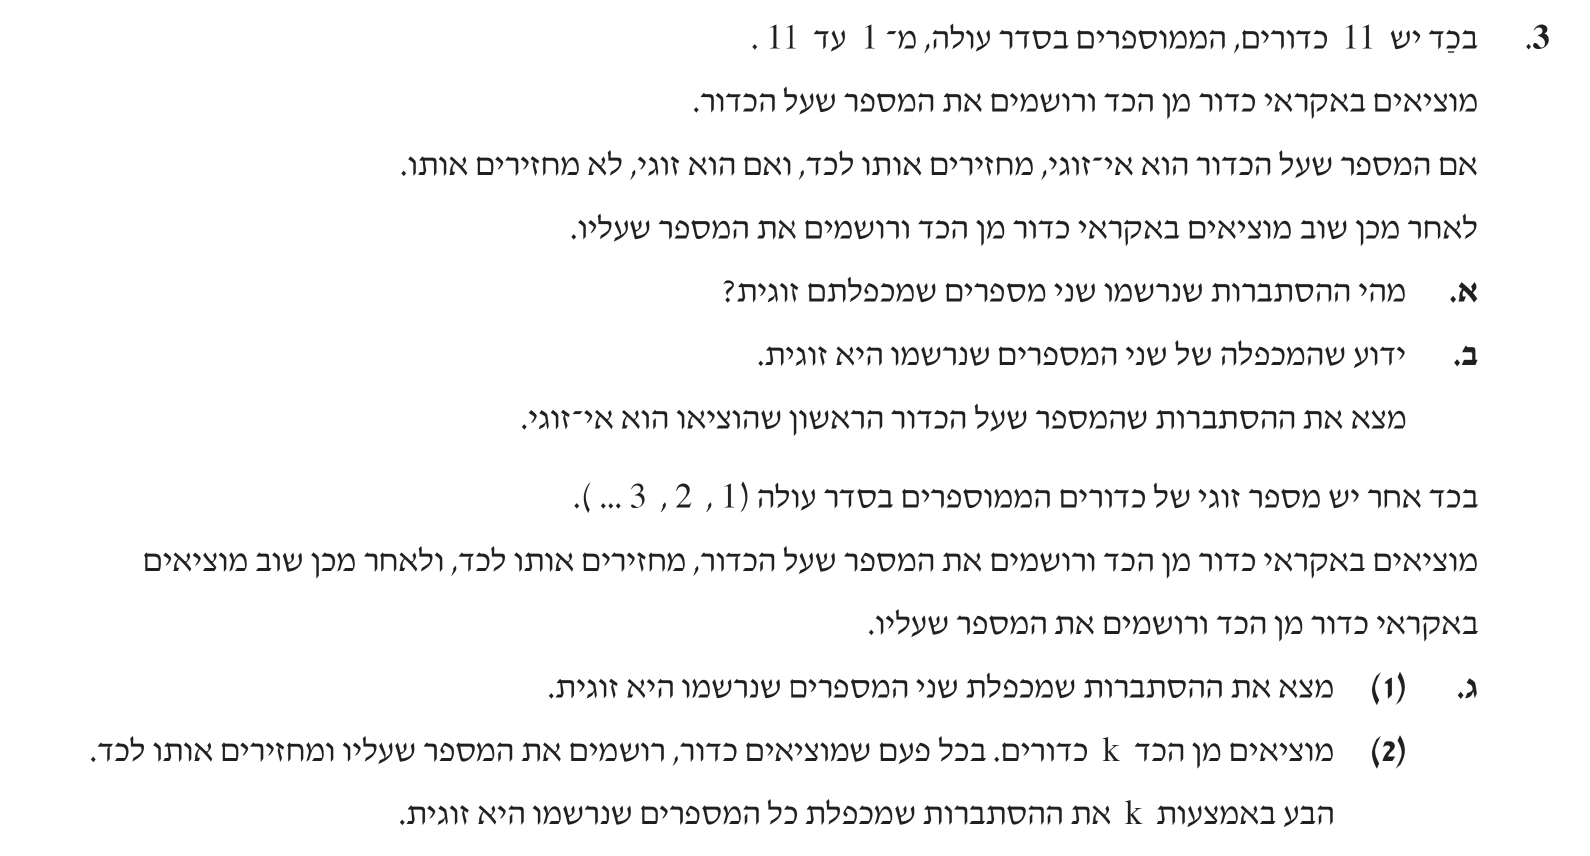
\includegraphics[width=.9\textwidth]{summer-2020a-3}
\end{center}

\textbf{סעיף א}

נסמן ב-%
$Z1,Z2$
את המאורעות של לשליפת כדור עם מספר זוגי בשליפה הראשונה והשנייה, נסמן ב-%
$I1,I2$
את המאורע של שליפת כדור אי-זוגי בשליפה הראשונה והשנייה ונסמן ב-%
$MZ$
את המאורע שהמכפלה של שני המספרים זוגית. מכפלה של שני מספרים שלמים היא זוגית אלא שניהם אי-זוגיים
$2k\cdot n = 2kn$
מספר זוגי ללא קשר לערך של 
$n$
אבל
$(2k+1)(2n+1)= 4kn + 2k + 2n +1$
הוא מספר אי-זוגי. השליפה של כדורים עם מספרים אי-זוגיים היא עם החזרה ולכן:
\[
P(MZ)=1-P(I1)P(I2)=1-\frac{6}{11}\cdot \frac{6}{11}=\frac{85}{121}\,.
\]

\textbf{סעיף ב}

המילה "ידוע" מכוון להסתברות מותנית. כדי להמכפלה תהיה זוגית כאשר המספר הראשון הוא אי-זוגי, השני חייב להיות זוגי. שוב נזכור שיש החזרה לאחר שליפת כדור עם מספר אי-זוגי ונקבל:
\[
P(I1/MZ) = \frac{P(I1\cap MZ)}{P(MZ)}= \frac{P(I1)P(Z2)}{P(MZ)}=
\frac{\frac{6}{11}\cdot\frac{5}{11}}{\frac{85}{121}}=\frac{6}{17}\,.
\]
שימו לב שלא השתמשנו בנתון שאין החזרה של שליפה של כדור עם מספר זוגי.

\textbf{סעיף ג 1}

בכד יש מספר שווה של כדורים עם מספרים זוגיים ועם אי-זוגיים ולכן ההסתברות לשלוף כדור עם מכפלה אי-זוגי היא 
$1-P(I1)P(I2)=1-\frac{1}{2}\cdot\frac{1}{2}=\frac{3}{4}$.

\textbf{סעיף ג 2}

מכפלת כל המספרים זוגית אלא אם כל 
$k$
המספרים הם אי-זוגיים, ולכן:
\[
P(MZ)=1-\left(\frac{1}{2}\right)^k\,.
\]

%%%%%%%%%%%%%%%%%%%%%%%%%%%%%%%%%%%%%%%%%%%%%%%%%%%%%%%%%

\section{חורף תש"פ}

\begin{center}
\selectlanguage{english}
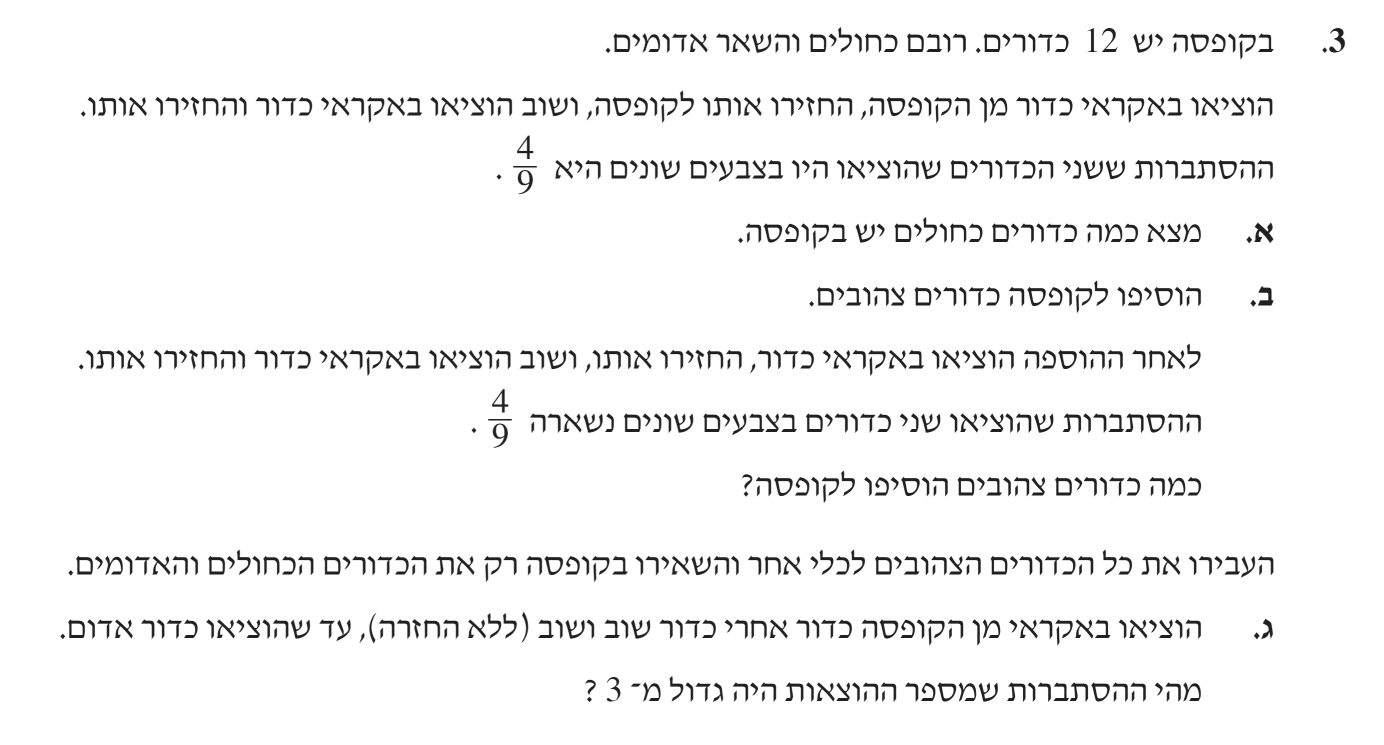
\includegraphics[width=.85\textwidth]{winter-2020-3}
\end{center}

\textbf{סעיף א}

נסמן ב-%
$K$ \L{(kahol)}
את המאורע של שליפת כדור כחול, נסמן ב-%
$A$ \L{(adom)}
את המאורע של שליפת כדור אדום ונסמן ב-%
$S$ \L{(shonim}
את המאורע של שליפת שני כדורים בצבעים שונים. שתי שליפות בלתי-תוליות של כדורים מכוון לעץ הסתברויות אבל המקרה כאן פשוט ונתקדם ישר לנוסחה. השליפה היא עם החזרה ולכן 
$P(KA)=P(AK)$
ההסתברות המבוקשת היא:
\begin{eqnarray*}
P(S) &=& P(KA) + P(AK) = 2P(KA) = 2\left(\frac{K}{12}\cdot \frac{A}{12}\right)=\frac{4}{9}\\
18KA &=& 4\cdot 144\\
KA &=& 32\,.
\end{eqnarray*}
בהתחשב באילוצים
$K+A=12, K>A$
הפתרון היחיד הוא
$K=8,A=4$.

\textbf{סעיף ב}

נסמן ב-%
$T$ \L{(tzahov)}
את המאורע של שליפת כדור צהוב. כמו בסעיף הקודם 
$P(KA)=P(AK)$, $P(KT)=P(TK)$, $P(AT)=P(TA)$.
ההסתברות המבוקשת היא:
\begin{eqnarray*}
P(S) &=& 2(P(KA)+P(KT)+P(AT))=\frac{4}{9}\\
&=&2\left(\frac{32}{(12+T)^2}+\frac{8T}{(12+T)^2}+\frac{4T}{(12+T)^2}\right)=\frac{4}{9}\\
54T+144 &=& T^2 + 24T + 144\\
T&=&30\,.
\end{eqnarray*}
$T=0$
הוא פתרון כי ברור שההסתברות לא משתנה אבל נניח שאכן מוסיפים מספר חיובי של כדורים.
\begin{center}
\begin{tikzpicture}
  [grow=right,
   level 1/.append style=
     {level distance=6em,sibling distance=4em},
   level 2/.append style=
     {level distance=6em,sibling distance=4em},
   level 3/.append style=
     {level distance=6em,sibling distance=4em}
  ]
  \node[left] {$(8,4)$}
    child {node[right]  {$(8,3)$}
        edge from parent node [below] {\R{אדום}} 
    }
    child {node [right] {$(7,4)$}
      child {node[right]  {$(7,3)$} 
          edge from parent node [below] {\R{אדום}}
      } 
      child {node[right]  {$(6,4)$}
        child {node[right]  {$(6,3)$}
            edge from parent node [below] {\R{אדום}}
        }
        child {node[right] {$(5,4)$}
            edge from parent node [above] {\R{כחול}}
        }
        edge from parent node [above] {\R{כחול}}
      }
      edge from parent node [above] {\R{כחול}}
    };
\end{tikzpicture}
\end{center}

\textbf{סעיף ג}

חזרנו למצב הראשון עם שמונה כדורים כחולים וארבעה אדומים. הדרך הקצרה לחשב את ההסתברות המבוקשת היא לחשב את ההסתברות המשלימה לשליפת כדור אדום בשליפה הראשונה, השנייה או השלישית. השליפה היא ללא החזרה ולכן ההסתברויות תלויות. ניתן לארגן את המידע בעץ (למעלה) כאשר בכל צומת רשום
$(K,A)$.
נסמן ב-%
$P(AR)$ \L{(adom rishon)}
את השליפה של הכדור האדום הראשון. ההסתברות המבוקשת היא:
\begin{eqnarray*}
P(AR) &=& 1-\left[P(A) + P(K)P(A) + P(K)P(K)P(A)\right]\\[6pt]
&=& 1-\left[\frac{4}{12} + \frac{8}{12}\cdot\frac{4}{11} +
   \frac{8}{12}\cdot\frac{7}{11}\cdot\frac{4}{10}\right]\\[6pt]
&=&1-\frac{984}{1320}=\frac{14}{55}\,.
\end{eqnarray*}

% !TeX root = probability.tex

%%%%%%%%%%%%%%%%%%%%%%%%%%%%%%%%%%%%%%%%%%%%%%%%%%%%%%%%%%%%%%

\section{קיץ תשע"ט מועד ב}

\begin{center}
\selectlanguage{english}
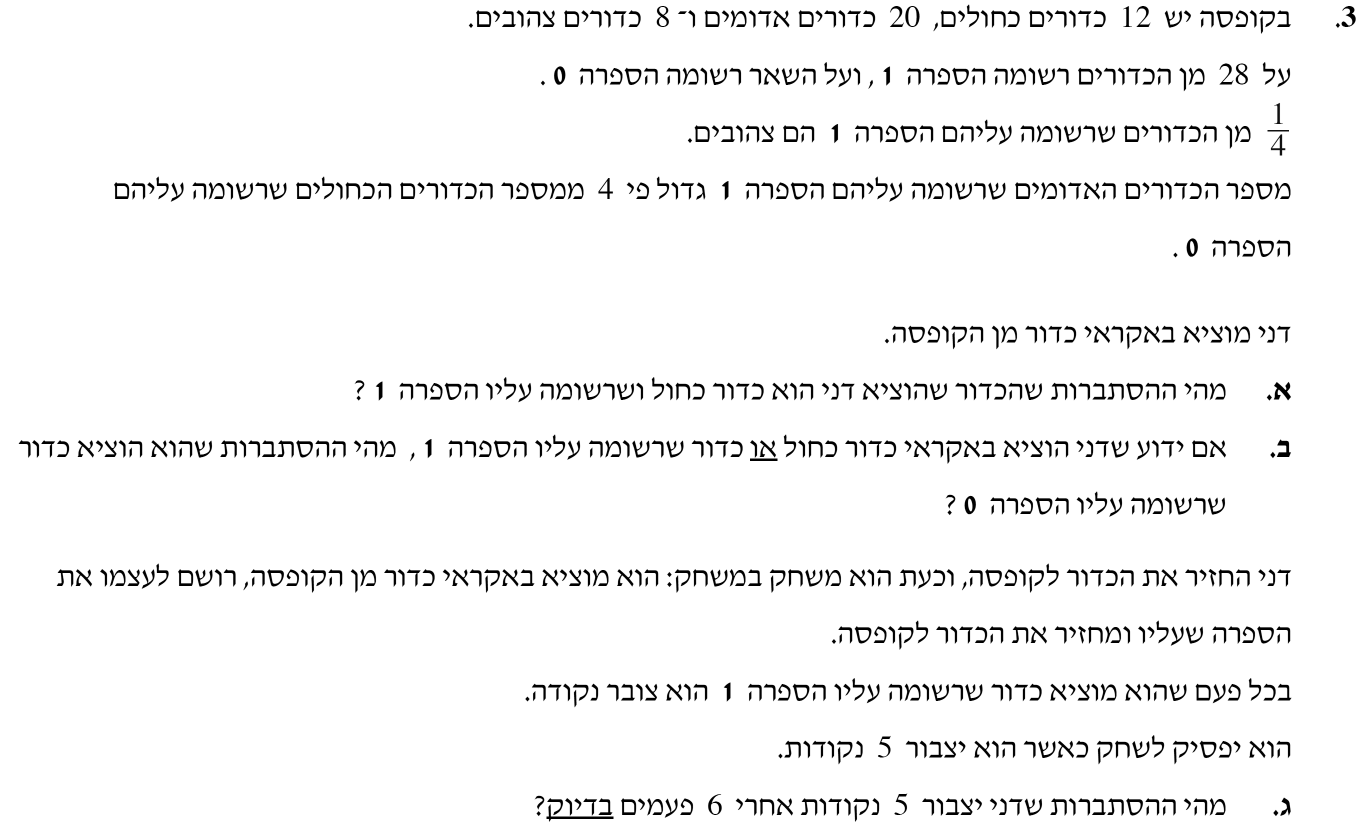
\includegraphics[width=.85\textwidth]{summer-2019b-3}
\end{center}

נסמן את המאורעות:
$K$
כדורים כפולים, 
$A$
כדורים אדומים,
$Z$
כדורים צהובים,
$0$
הספרה אפס,
$1$
הספרה אחד. השאלה שואלת על מאורעות המורכבים משני סוגי מאורעותת פשוטים יותר, צבעים וספרות, ולכן נארגן את המידע בטבלה.%
\footnote{%
באתר של יואל גבע הפתרון מתבסס על עץ. לדעתי שיטה זו מתאימה יותר כאשר יש מאורעות עוקבים, כגון שליפת הצבע מקופסה אחת ואחר כך שליפת הספרה מקופסה שנייה. כאן כאשר הניסוי הוא שליפה של כדור אחד עדיף להשתמש בטבלה.} בטבלה נרשום מספרים שלמים כאשר הכוונה של המספר 
$n$
הוא 
$P(n/40)$.

מספר הכדורים מכל צבע נתון ונתון גם שרבע מהכדורים שרשומה עליהם 
$1$
הם צהובים. ממידע זה ניתן למלא את התאים בטבלה בהם מופיעים מספרים שלמים. נסמן בנעלם
$X$
את מספרם של הכדורים הכחולים שרשומה עליהם אפס. לפי היחס הנתון בין 
$X$
לבין מספר הכדורים האדומים שרשומה עליהם אחד ניתן להשלים את הטבלה. מהתאים עבור הכדורים האדומים נקבל משוואה
$4X+11-X=20$
ולכן 
$X=3$.

\begin{center}
\selectlanguage{english}
\begin{tikzpicture}[scale=1.25]
\draw (0,0) grid[xstep=1.2cm] (4.8,3);
\node at (4.2,3.3) {$\bm{T}$};
\node at (3,3.3) {$\bm{A}$};
\node at (1.8,3.3) {$\bm{K}$};
\node at (5.3,2.5) {$\bm{1}$};
\node at (5.3,1.5) {$\bm{0}$};

\node at (4.2,2.5) {$7$};
\node at (3,2.5) {$4X$};
\node at (1.8,2.5) {$21\!-\!4X$};
\node at (0.6,2.5) {$28$};

\node at (4.2,1.5) {$1$};
\node at (3,1.5) {$11\!-\!X$};
\node at (1.8,1.5) {$X$};
\node at (0.6,1.5) {$12$};

\node at (4.2,0.5) {$8$};
\node at (3,0.5) {$20$};
\node at (1.8,0.5) {$12$};
\node at (0.6,0.5) {$40$};

\end{tikzpicture}
\end{center}

\newpage

נציב 
$X=3$
ונקבל מספרים בכל התאים:
\begin{center}
\selectlanguage{english}
\begin{tikzpicture}[scale=1.25]
\draw (0,0) grid[xstep=1.2cm] (4.8,3);
\node at (4.2,3.3) {$\bm{T}$};
\node at (3,3.3) {$\bm{A}$};
\node at (1.8,3.3) {$\bm{K}$};
\node at (5.3,2.5) {$\bm{1}$};
\node at (5.3,1.5) {$\bm{0}$};

\node at (4.2,2.5) {$7$};
\node at (3,2.5) {$12$};
\node at (1.8,2.5) {$9$};
\node at (0.6,2.5) {$28$};

\node at (4.2,1.5) {$1$};
\node at (3,1.5) {$0$};
\node at (1.8,1.5) {$3$};
\node at (0.6,1.5) {$12$};

\node at (4.2,0.5) {$8$};
\node at (3,0.5) {$20$};
\node at (1.8,0.5) {$12$};
\node at (0.6,0.5) {$40$};

\end{tikzpicture}
\end{center}
\textbf{סעיף א}

מהטבלה נקבל
$P(K \cap 1) = \frac{9}{40}$.

\textbf{סעיף ב}

"אם ידוע" מכוון להתסברות מותנית:
\[
P(0/ K\:\cup\: 1) = \frac{P(0 \cap (K\:\cup\:1))}{P(K\:\cup\:1))}\,.
\]
אפשר לפתח את הביטוי לפי חוק הפילוג לקבוצות אבל פשוט נשים לב שלא יכול להיות כדור שרשומה עליו גם אפס וגם אחד, ולכן:
\[
P(0/ K\:\cup\: 1) = \frac{P(0 \cap K)}{P(K\:\cup\:1))}
= \frac{3}{12+28-9}=\frac{3}{31}\,.
\]
כאשר מחשבים את איחוד הקבוצות
$K, 1$
על ידי סכום מספר האיברים בקבוצה 
$K$
ומספר האיברים בקבוצה
$1$,
אנו סופרים את האיברים ב-%
$K\cap1$
פעמיים ולכן יש להחסיר את מספר האיברים בקבוצה זו.

\textbf{סעיף ג}

המילה "בדיוק" מכוון לנוסחת ברנולי אבל יש כאן מלכודת. לו שאלו מה ההסתברות לצבור חמש נקודות בחמשה סיבובים הפתרון מתקבל מנוסחת ברנולי פשוט. אבל כדי לקבל חמש נקודות בששה סיבובים חייבים להפסיד בסיבוב אחד בדיוק מבין חמשת הסיבובים הראשונים ורק אז לזכות בנקודה בסיבוב האחרון. אחרת, המשחק היה נפסק לאחר הסיבוב החמישי. נסמן ב-%
$k/n$
את המאורע של לזכות ב-%
$k$
נקודות מתוך 
$n$
סיבובים:
\[
P(\textrm{\R{זכייה חמישית בסיבוב הששי}})=P(4/5) P(1/1)=
{5 \choose 1}\left(\frac{12}{40}\right)^1\left(\frac{28}{40}\right)^4\left(\frac{28}{40}\right)^1=0.252015\,.
\]

%%%%%%%%%%%%%%%%%%%%%%%%%%%%%%%%%%%%%%%%%%%%%%%%%%%%%%%%%%%%%

\section{קיץ תשע"ט מועד א}

\begin{center}
\selectlanguage{english}
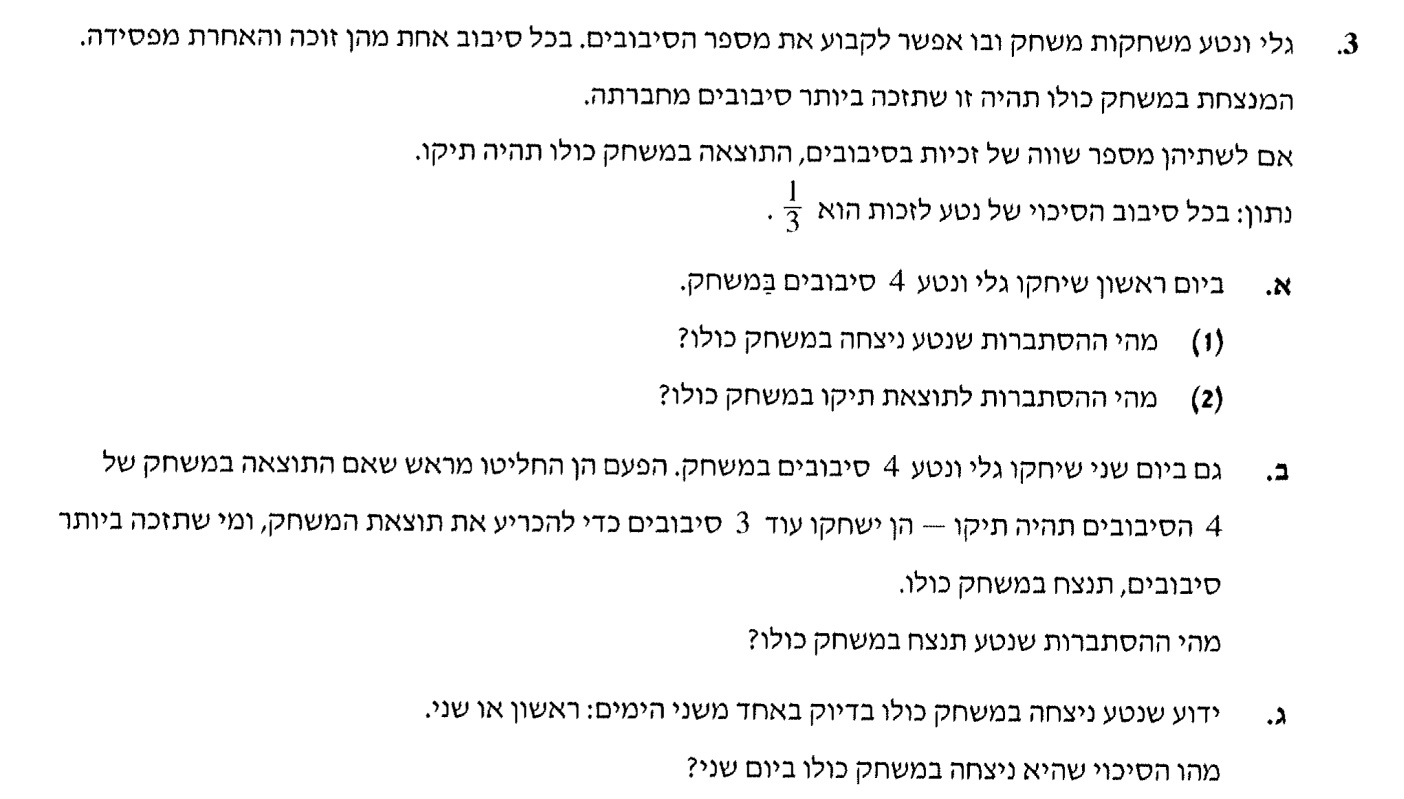
\includegraphics[width=.9\textwidth]{summer-2019a-3}
\end{center}

משחק בסיבובים מכוון לנוסחת ברנולי.

\textbf{סעיף א 1}

נסמן את המאורע שנטע ניצחה בסיבוב ב-%
$N$
והמאורע שנטע ניצחה במחשק ב-%
$M$.
\[
P(M) = P(N=3 \:\cup\: N=4)=P(N=3)+P(N=4)\,,
\]
כי במאורעות בלתי-תלויים: אי-אפשר לנצח גם בשלושה סיבובים וגם בארבעה. לפי נוסחת ברנולי:
\[
P(M)={4\choose 3}\left(\frac{1}{3}\right)^3\left(\frac{2}{3}\right)^1+
{4\choose 4}\left(\frac{1}{3}\right)^4\left(\frac{2}{3}\right)^0=
\frac{8}{81}+\frac{1}{81}=\frac{9}{81}=\frac{1}{9}\,.
\]

\textbf{סעיף א 2}

כדי להגיע לתיקו נטע חייבת לנצח בדיוק בשני סיבובים:
\[
P(N=2)={4\choose 2}\left(\frac{1}{3}\right)^2\left(\frac{2}{3}\right)^2=\frac{24}{81}=\frac{8}{27}\,.
\]

\textbf{סעיף ב}

נטע מנצחת במשחק אם היא מנצחת בארבעה סיבובים או שיש תיקו ואחכ כך היא מנצחת בשניים מתוך שלושה סיבובים. נשתמש בתוצאות של סעיף א ונקבל:
\begin{eqnarray*}
P(M)&=&\frac{1}{9}+\frac{8}{27}
  \left[{3\choose 2}\left(\frac{1}{3}\right)^2\left(\frac{2}{3}\right)^1  +
  {3\choose 3}\left(\frac{1}{3}\right)^3\left(\frac{2}{3}\right)^0
  \right]\\
  &=&\frac{1}{9}+\frac{8}{27}
  \left[ \frac{6}{27} + \frac{1}{27} \right]=
  \frac{81}{729}+\frac{56}{729}=\frac{137}{729}\,.
\end{eqnarray*}

\textbf{סעיף ג}

חייבים לשים לב לניסוח בסעיף ב': המשחק עם שבעה סיבובים מתרחש רק ביום שני כאשר ביום ראשון המחשק נשאר עם ארבעה סיבובים. נסכם את מה שיש לנו כאשר 
$N1, N2$
מסמנים שנטע ניצחה ביום ראשון ויום שני בהתאמה:
\[
P(N1) = \frac{1}{9},\quad P(\overline{N1})=\frac{8}{9},\quad 
P(N2) = \frac{137}{729}, \quad P(\overline{N2})=\frac{592}{729}\,.
\]
נניח ששני המשחקים בלתי-תלויים כך שאפשר להכפיל את ההסתברויות שלהם. 
נסמן ב-%
$1$
את המאורע שנטע מנצחת רק באחד משני המשחקים ונשמתש בעובדה ש-%
$(\overline{N1}\cup N2) \subseteq 1$,
כי ניצחון של נטע רק במשחק בשני הוא אחד המקרים של נטע מנצחת רק במשחק אחד. נחשב את ההסתברות המבוקשת:
\begin{eqnarray*}
P(\overline{N1}\cup N2) / 1) &=& 
\frac{P((\overline{N1}\cup N2) \cap 1)}{P(1)}\\
&=& \frac{P(\overline{N1})P(N2)}
{P(\overline{N1})P(N2)+P(N1)P(\overline{N2})}\\[8pt]
&=&\frac{\disfrac{8}{9}\cdot \frac{137}{729}}
{\disfrac{8}{9}\cdot \frac{137}{729}+\disfrac{1}{9}\cdot \frac{592}{729}}\\[8pt]
&=&\frac{8\cdot 137}{8\cdot 137+592}=\frac{1096}{1688}=0.6493\,.
\end{eqnarray*}

%%%%%%%%%%%%%%%%%%%%%%%%%%%%%%%%%%%%%%%%%%%%%%%%%%%%%%%%%

\newpage

\section{חורף תשע"ט}

\begin{center}
\selectlanguage{english}
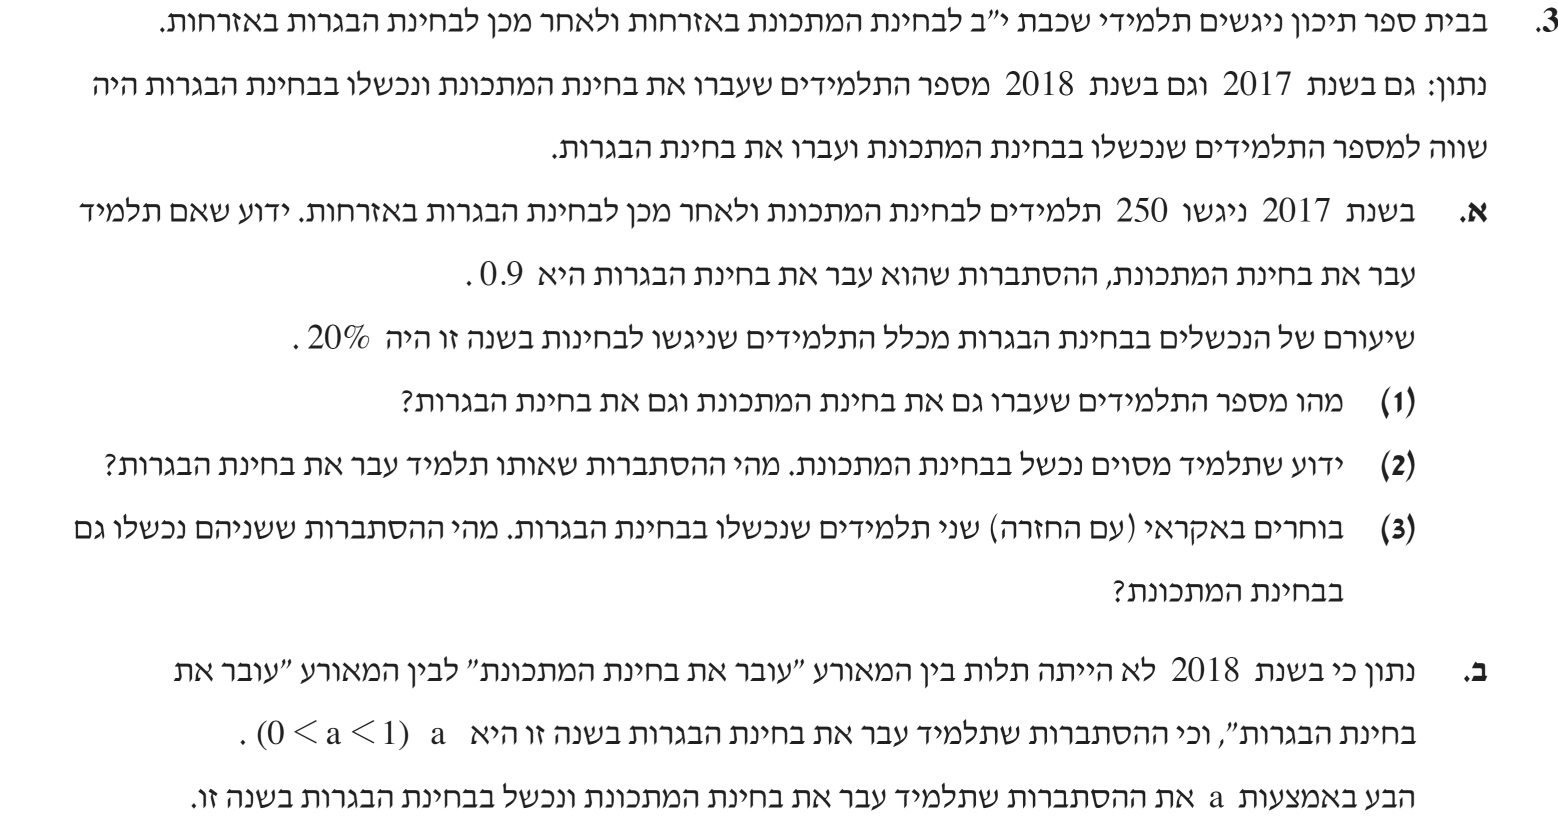
\includegraphics[width=.85\textwidth]{winter-2019-3}
\end{center}

השאלה שואלת על שני סוגי של מאורעות שמכוון לאירגון המידע בטבלה. נסמן ב-%
$B$ \L{bagrut}
את המאורע של הצלחה בבגרות ונסמן ב-%
$M$ \L{matkonet}
את המאורע של הצלחה במתכונת.

נתון שמספר הנכשלים בבגרות הוא 
$0.20$
ומהסתברות משלימה מספר העוברים הוא
$0.80$.
נתון גם ש:
\[
P(B\cap\overline{M})=P(\overline{B}\cap M)\,,
\]
ונסמן נעלם זה ב-%
$X$
ונסמן את הנעלם
$P(M)$
ב-%
$Y$.

המילה "ידוע" מכוון להסתברות מותנית:
\begin{eqnarray*}
P(B/M)&=&\frac{P(B\cap M)}{P(M)}=0.90\\
P(B\cap M)&=&0.90 P(M)=0.90Y\,.
\end{eqnarray*}
כעת ניתן למלא את כל תאי הטבלה:
\begin{center}
\selectlanguage{english}
\begin{tikzpicture}[scale=1.25]
\draw (0,0) grid[xstep=1.5] (4.5,3);
\node at (3.75,3.3) {$B$};
\node at (2.25,3.3) {$\overline{B}$};
\node at (5,2.5) {$M$};
\node at (5,1.5) {$\overline{M}$};

\node at (3.75,2.5) {$0.90Y$};
\node at (2.25,2.5) {$X$};
\node at (0.75,2.5) {$Y$};

\node at (3.75,1.5) {$X$};
\node at (2.25,1.5) {$1\!-\!Y\!-\!X$};
\node at (0.75,1.5) {$1\!-\!Y$};

\node at (0.75,0.5) {$1.0$};
\node at (2.25,0.5) {$0.20$};
\node at (3.75,0.5) {$0.80$};
\end{tikzpicture}
\end{center}

מהעומדות של הבגרות נקבל שתי משוואות:
\begin{eqnarray*}
0.90Y+X&=&0.80\\
X+1-Y-X&=&0.20\\
Y&=&0.80\\
X&=&0.08\,.
\end{eqnarray*}
ניתן למלא אל כל התאים במספרים:
\begin{center}
\selectlanguage{english}
\begin{tikzpicture}[scale=1.25]
\draw (0,0) grid[xstep=1.5] (4.5,3);
\node at (3.75,3.3) {$B$};
\node at (2.25,3.3) {$\overline{B}$};
\node at (5,2.5) {$M$};
\node at (5,1.5) {$\overline{M}$};

\node at (3.75,2.5) {$0.72$};
\node at (2.25,2.5) {$0.08$};
\node at (0.75,2.5) {$0.80$};

\node at (3.75,1.5) {$0.08$};
\node at (2.25,1.5) {$0.12$};
\node at (0.75,1.5) {$0.20$};

\node at (0.75,0.5) {$1.0$};
\node at (2.25,0.5) {$0.20$};
\node at (3.75,0.5) {$0.80$};
\end{tikzpicture}
\end{center}

\textbf{סעיף א 1}

מהטבלה
$P(B\cap M)=0.72$
ומספר הנבחנים
$250=$
ולכן מספר העוברים את שתי הבחינות
$180=$.

\textbf{סעיף א 2}

\[
P(B/\overline{M})=\frac{P(B\cap\overline{M})}{P(\overline{M})}=
\frac{0.08}{0.2}=0.4\,.
\]

\textbf{סעיף א 3}

\[
P(\overline{M}/\overline{B})=\frac{P(\overline{M}\cap \overline{B})}{P(\overline{B})}=\frac{0.12}{0.2}=0.6\,.
\]

\textbf{סעיף ב}

בתחילת השאלה כתוב ש-%
$P(M\cap\overline{B})=P(\overline{M}\cap B)$
גם עבור שנת 2018. המאורעות
$M,B$
בלתי-תלויים ולכן גם המאורעות
$M,\overline{B}$
ו-%
$\overline{M},B$.
נמצא בחישוב את הביטוי המבוקש ל-%
$P(M\cap\overline{B})$:
\begin{eqnarray*}
P(M) P(\overline{B})&=&P(M\cap\overline{B})=
P(\overline{M}\cap B)=P(\overline{M})P(B)\\
P(M)(1-a)&=&(1-P(M))a\\
P(M)&=&a\\
P(M\cap\overline{B})&=&P(M)P(\overline{B})=a(1-a)=a-a^2\,.
\end{eqnarray*}

% !TeX root = probability.tex

%%%%%%%%%%%%%%%%%%%%%%%%%%%%%%%%%%%%%%%%%%%%%%%%%%%%%%%%%%%%%

\addcontentsline{toc}{section}{\large בחינות ופתרונות}

\section{קיץ תשע"ח מועד ב}

\begin{center}
\selectlanguage{english}
\hspace*{8em}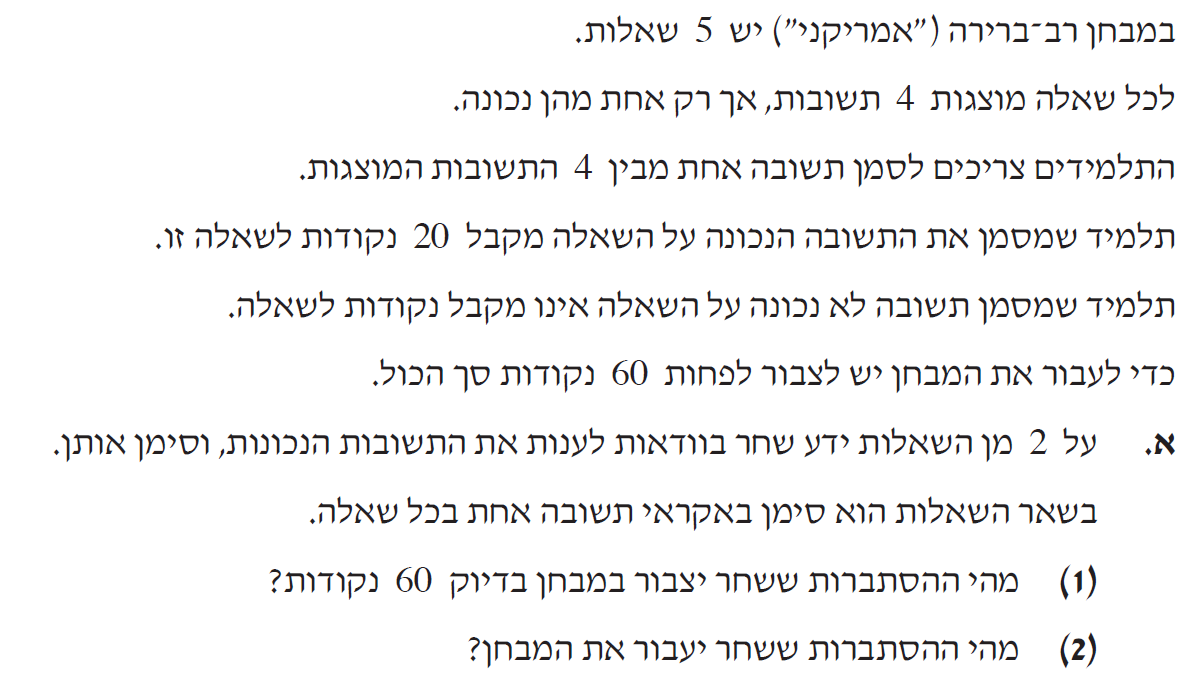
\includegraphics[width=.7\textwidth]{summer-2018b-3a}
\hspace*{-2.2em}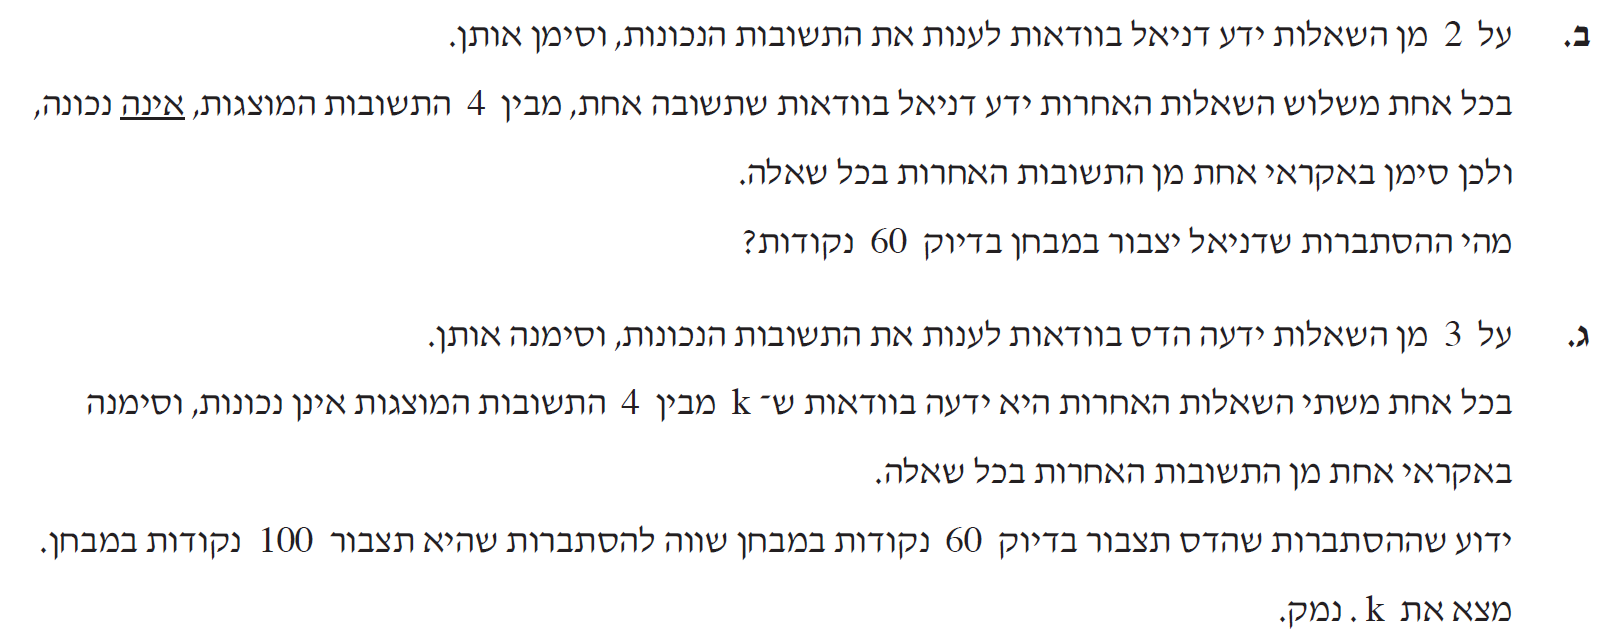
\includegraphics[width=\textwidth]{summer-2018b-3b}
\end{center}

המאורועות הם מספר הנקודות הצברות על ידי התלמידים.

השאלה מתארת הצלחות וכשלונות במתן לתשובות על המבחן ושואלת על מספר ההצלחות והכשלונות. לכן הפתרון ישתמשמ בנוסחת ברנולי.

\textbf{סעיף א}

1. שחר ידע שהוא ענה נכון על שתי שאלות ולכן כדי לקבל ציון
$60$
עליו לענות על בדיוק אחת משלושת השאלות האחרות. ההסתברות לענות נכון על שאלה היא 
$\frac{1}{4}$
ולפי נוסחת ברנולי:
\[
{3 \choose 1}\left(\frac{1}{4}\right)\left(\frac{3}{4}\right)^2=\frac{27}{64}\,.
\]
2. כדי לעבור את המבחן עליו לצבור לפחות שלוש תשובות נכונות. להסתברות מהסעיף הקודם יש להוסיף את ההסתברויות של ארבע וחמש תשובות נכונות:
\[
\frac{27}{64}+{3 \choose 2}\left(\frac{1}{4}\right)^2\left(\frac{3}{4}\right)^1+{3 \choose 3}\left(\frac{1}{4}\right)^3\left(\frac{3}{4}\right)^0=\frac{37}{64}\,.
\]

\newpage

\textbf{סעיף ב}

דניאל צריך לענות נכון על שאלה אחת בדיוק מתוך שלושת השאלות הנותרות. דניאל ידע שתשובה אחת לא נכונה, לכן ההסתברות שהוא ענה נכון על השאלה היא
$\frac{1}{3}$
ולא 
$\frac{1}{4}$
כמו בסעיף הקודם:
\[
{3 \choose 1}\left(\frac{1}{3}\right)\left(\frac{2}{3}\right)^2=\frac{4}{9}\,.
\]
\textbf{סעיף ג}

תהי
$p_k$
ההסתברות שהדס ידעה וודאות ש-%
$k$
מתוך 
$4$
תשובות לא נכונות. ההסתברות שהיא שהיא צריכה לבחור תשובה באופן אקראי היא המשלים
$1-p_k$.
כדי לקבל ציון
$60$
היא צריכה לענות נכון על אפס מתוך שתי השאלות הנוספות וכדי לקבל ציון 
$100$
היא צריכה לענות נכון על כל השאלות הנכונות. נשווה את שתי ההסתברויות המתקבלות מנוסחת ברנולי:
\begin{eqnarray*}
{2 \choose 0}p_k^0(1-p_k)^2 &=& {2 \choose 2}p_k^2(1-p_k)^0\\
(1-p_k)^2 &=& p_k^2\\
p_k&=&\frac{1}{2}\,,
\end{eqnarray*}
כאשר השתמשנו ב-%
${n\choose 0}={n\choose n}=1$
ו-%
$p^0=(1-p)^0=1$.

 ההסתברות שהיא ענתה תשובה נכונה לשאלה אחת היא
$p_k=\displaystyle\frac{1}{4-k}$
ולכן 
$k=2$.

\textbf{פתרון שני}

אם לא היינו מגדירים את הסימון
$p_k$
היינו מקבלים מפישוט השוויון של נוסחאות ברנולי:
\[
\left(\frac{1}{4-k}\right)^2 =\left(1-\frac{1}{4-k}\right)^2=\left(\frac{3-k}{4-k}\right)^2\,.
\]
נכפיל את שני הצדדים של המשוואה ב-%
$(4-k)^2$
ונקבל את המשוואה ריבועית
$k^2-6k+8=0$
שפתרונותיה הם 
$k=2,k=4$.
הפרמטר
$k$
מוגדר כמספר התשובות שהדס יודעת שהן אינן נכונות, ונתון שתשובה אחת נכונה, כך שיש לפסול את הפתרון
$k=4$
ולבחור
$k=2$.

האפשרות השנייה היא לקחת שורש של שני הצדדים ונקבל שתי משוואות:
\begin{eqnarray*}
\frac{1}{4-k}&=&+\frac{3-k}{4-k}\\
\frac{1}{4-k}&=&-\frac{3-k}{4-k}\,.
\end{eqnarray*}
מהמשוואה הראשונה נקבל
$k=2$.
מהמנה של המשוואה השנייה נקבל 
$k=4$
ונפסול אותו כי הוא מאפס את המכנה.

כל הפתרונות מגיעים לתשובה הנכונה אבל בחירה נכונה של סימון וסדר החישובים יכולים להשפוע על פשטות הפתרון.

%%%%%%%%%%%%%%%%%%%%%%%%%%%%%%%%%%%%%%%%%%%%%%%%%%%%%%%%%%%%%%

\newpage

\section{קיץ תשע"ח מועד א}

\begin{center}
\selectlanguage{english}
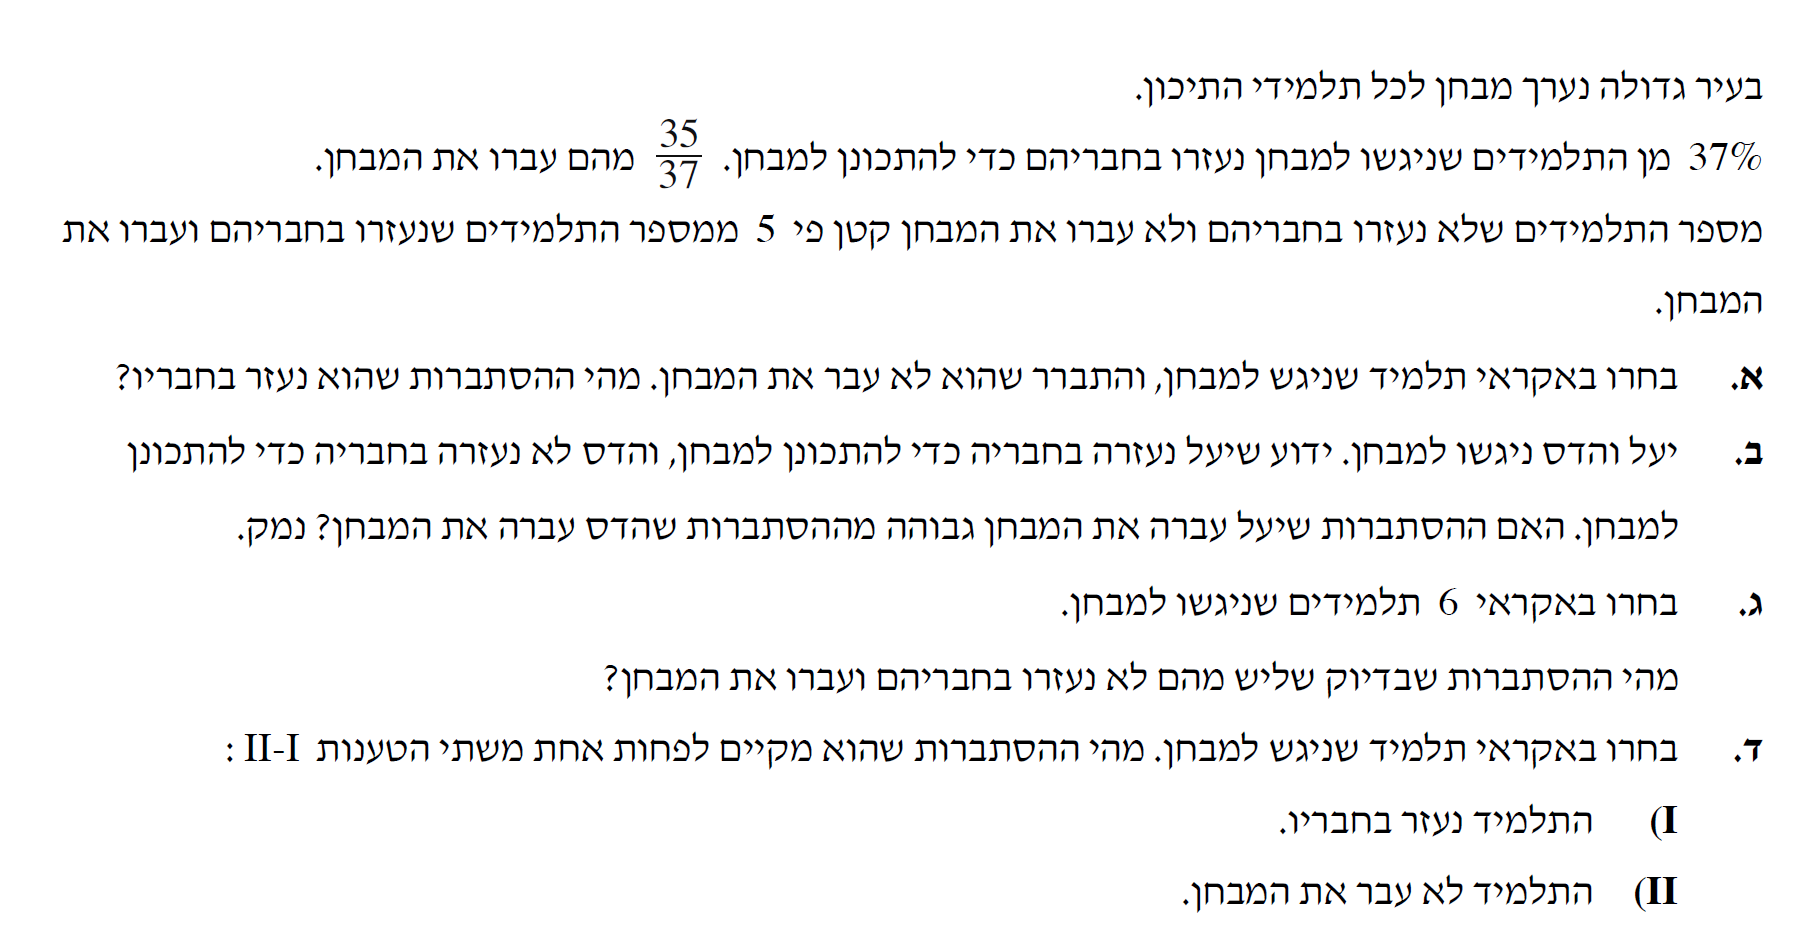
\includegraphics[width=	\textwidth]{summer-2018a-3}
\end{center}

מצאתי שניסוח השאלה מבלבל. כאשר כתוב ש-%
$37\%$
מן התלמידים ניגשו למבחן, הנטייה היא לפרש את זה כ-%
$37$
מתוך
$100$
תלמידים, כאשר אחוז למעשה מבטא יחס:
\[
37\% = \frac{37}{100} = \frac{74}{200} = \frac{18.5}{50} = \cdots\,.
\]
המשפט הבא קובע ש-%
$\frac{35}{37}$
"מהם" עברו את המבחן ואפשר לחשוב שמדובר ב-%
$35$
מתוך
$37$
תלמידים, אולם שוב מדובר ביחס. בשני המקרים יחס הוא הסתברות.

נסמן ב-%
$N$ 
\L{(ne-ezru)}
את התלמידים שנעזרו בחבריהם, וב-%
$A$
\L{(avru)}
את התלמידים שעברו את המבחן. המאורעות מורכבים משתי קבוצות הללו, משלימהם וחיתוכים שלהם, לכן נבחר היעזר בטבלה כדי לייצג את הנתונים. 
לפני שניגש לפתור את השאולות בסעיפים, נמלא את טבלת ההסתברויות לפי המידע הנתון.

\textbf{בניית הטבלה}

נתון ש-%
$P(N)=\frac{37}{100}$.
השימוש במילה
"\textbf{מהם}"
מכוון להסתברות מותנית כך ש:
\[
P(A/N)=\frac{35}{37}
\]
ולכן:
\begin{eqnarray*}
P(A/N) &=& \frac{P(N\cap A)}{P(N)}\\
P(N\cap A) &=& P(A/N)\cdot P(N) = \frac{35}{37}\cdot \frac{37}{100} = \frac{35}{100} = 0.35\,.
\end{eqnarray*}
נשתמש במשלימים להסתברויות ונקבל:
\begin{center}
\selectlanguage{english}
\begin{tikzpicture}[scale=1.25]
\draw (0,0) grid (3,3);
\node at (2.5,3.3) {$\bm{A}$};
\node at (1.5,3.3) {$\bover{A}$};
\node at (3.3,2.5) {$\bm{N}$};
\node at (3.3,1.5) {$\bover{N}$};
\node at (2.5,2.5) {$0.35$};
\node at (0.5,2.5) {$0.37$};
\node at (1.5,2.5) {$0.02$};
\node at (0.5,1.5) {$0.63$};
\node at (0.5,0.5) {$1.0$};
\end{tikzpicture}
\end{center}



בהמשך נתון ש:
\[
P(\overline{N}\cap\overline{A})=\frac{P(N\cap A)}{5}=\frac{0.35}{5}=0.07\,,
\]
וניתן להשלים את הטבלה:
\begin{center}
\selectlanguage{english}
\begin{tikzpicture}[scale=1.25]
\draw (0,0) grid (3,3);
\node at (2.5,3.3) {$\bm{A}$};
\node at (1.5,3.3) {$\bover{A}$};
\node at (3.3,2.5) {$\bm{N}$};
\node at (3.3,1.5) {$\bover{N}$};
\node at (2.5,2.5) {$0.35$};
\node at (0.5,2.5) {$0.37$};
\node at (1.5,2.5) {$0.02$};
\node at (0.5,1.5) {$0.63$};
\node at (0.5,0.5) {$1.0$};
\node at (1.5,0.5) {$0.09$};
\node at (2.5,0.5) {$0.91$};
\node at (1.5,1.5) {$0.07$};
\node at (2.5,1.5) {$0.56$};
\end{tikzpicture}
\end{center}

\smallskip

\textbf{סעיף א}

הניסוח "בחרו 
$\ldots$
תלמיד 
$\ldots$
שלא עבר את המבחן. מה ההסתברות
\textbf{שהוא}
נעזר בחבריו?" מכוון להסתברות מותנית:
\[
P(N/\overline{A})=\frac{P(N\cap \overline{A})}{P(\overline{A})}=\frac{0.02}{0.09}=\frac{2}{9}\,.
\]
\textbf{סעיף ב}

הניסוח
\textbf{"ידוע ש"}
מכוון להסתברות מותנית.

עבור יעל ההסתברות המותנית היא:
\[
P(A/N)=\frac{P(A \cap N)}{P(N)}=\frac{0.35}{0.37}=0.9459\,,
\]
ועבור הדס ההסתברות המותנית היא:
\[
P(A/\overline{N})=\frac{P(A\cap \overline{N})}{P(\overline{N})}=\frac{0.56}{0.63}=0.8889\,.
\]
ליעל הסתברות גבוהה יותר לעבור את המבחן.

\smallskip

\textbf{סעיף ג}

שליש (לא שלושה!) של שש הוא שניים. המילה "בדיוק" מכוון לנוסחת
ברנולי הערך
$P(\overline{N}\cap A)=0.56$
נמצא בטבלה ולפי נוסחה ברנולי ההסתברות היא:
\[
{6 \choose 2}(0.56)^2 (1-0.56)^4=0.1763\,.
\]
\textbf{סעיף ד}

הניסוח
"\textbf{לפחות אחת}"
משתי הטענות
\L{I, II}
אומר שמאורע מורכב משני המאורעות
\L{I, II}
או משניהם. בתרשים להלן שני העגולים המייצגים את שני המאורעות
\L{I, II}
כאשר המאורע "לפחות אחת" מיוצג על ידי כל השטח המקווקו:
\begin{center}
\selectlanguage{english}
\begin{tikzpicture}
\begin{scope}
\clip[draw] (0,0) circle[radius=2];
\foreach \y in {-1.5,-1,-.5,0,.5,1,1.5}
  \draw (-2,\y) -- (2,\y);
\end{scope}
\begin{scope}
\clip[draw] (2.5,0) circle[radius=2];
\foreach \x in {1,1.5,2,2.5,3,3.5,4}
  \draw (\x,-2) -- (\x,2);
\end{scope}
\node at (-2,2.5) {\textrm{I}};
\node at (4.5,2.5) {\textrm{II}};
\node at (1.25,2.5) {\textrm{I}$\:\cap\:$\textrm{II}};
\node at (-3.5,.2) {\textrm{I$-$II}};
\node at (6,.2) {\textrm{II$-$I}};
\draw[->] (1.25,2.2) -- ++(0,-1);
\draw[->] (-3,.2) -- ++(1.7,0);
\draw[->] (5.5,.2) -- ++(-1.7,0);
\draw[->] (-2,2.2) -- +(.6,-.6);
\draw[->] (4.5,2.2) -- +(-.6,-.6);
\end{tikzpicture}
\end{center}
יש שתי דרכים לחשב את ההסתברות. בדרך הראשונה אנו לוקחים את סכום ההסתברויות של שני המאורעים, ומחסירים את ההסתברות של המאורע המשותף כי ספרנו אותו פעמיים, פעם כחלק מהמאורע
\L{I}
ופעם כחלק מהמאורע
\L{II}:
\[
P(\textrm{I} \cup \textrm{II}) = P(\textrm{I}) + P(\textrm{II}) - P(\textrm{I} \cap \textrm{II})\,.
\]
בדרך השניה אנו סופרים כל חלק מהמאורע השותף בנפרד, כאשר הסימון
\L{I-II}
הוא כל האיברים בקבוצה 
\L{I}
שאינם בקבוצה
\L{II}
ולהיפך:
\[
P(\textrm{I} \cup \textrm{II}) = P(\textrm{I}\:-\:\textrm{II}) + P(\textrm{II}\:-\:\textrm{I}) + P(\textrm{I} \cap \textrm{II})\,.
\]
את ההסתברויות לחישוב ניקח מהטבלה. הדרך הראשונה מופיעה מימין והדרך השניה משמאל:
\begin{center}
\selectlanguage{english}
\begin{tikzpicture}[scale=1.25]
\begin{scope}
\draw (0,0) grid (3,3);
\node at (2.5,3.3) {$\bm{A}$};
\node at (1.5,3.3) {$\bover{A}$};
\node at (3.3,2.5) {$\bm{N}$};
\node at (3.3,1.5) {$\bover{N}$};
\node at (2.5,2.5) {$0.35$};
\node at (0.5,2.5) {$0.37$};
\node at (1.5,2.5) {$0.02$};
\node at (0.5,1.5) {$0.63$};
\node at (0.5,0.5) {$1.0$};
\node at (1.5,0.5) {$0.09$};
\node at (2.5,0.5) {$0.91$};
\node at (1.5,1.5) {$0.07$};
\node at (2.5,1.5) {$0.56$};
\draw[ultra thick] (2,2) rectangle +(1,1);
\draw[ultra thick] (1,1) rectangle +(1,1);
\draw[ultra thick] (1,2) rectangle +(1,1);
\end{scope}
\begin{scope}[xshift=6cm]
\draw (0,0) grid (3,3);
\node at (2.5,3.3) {$\bm{A}$};
\node at (1.5,3.3) {$\bover{A}$};
\node at (3.3,2.5) {$\bm{N}$};
\node at (3.3,1.5) {$\bover{N}$};
\node at (2.5,2.5) {$0.35$};
\node at (0.5,2.5) {$0.37$};
\node at (1.5,2.5) {$0.02$};
\node at (0.5,1.5) {$0.63$};
\node at (0.5,0.5) {$1.0$};
\node at (1.5,0.5) {$0.09$};
\node at (2.5,0.5) {$0.91$};
\node at (1.5,1.5) {$0.07$};
\node at (2.5,1.5) {$0.56$};
\draw[ultra thick] (0,2) rectangle +(1,1);
\draw[ultra thick] (1,0) rectangle +(1,1);
\draw[ultra thick] (1,2) rectangle +(1,1);
\end{scope}
\end{tikzpicture}
\end{center}
בשתי הדרכים מקבלים אותה תוצאה:
\begin{eqnarray*}
P(N\cup\overline{A})&=&P(N) + P(\overline{A}) - P(N\cap\overline{A}) = 0.37+0.09-0.02=0.44\\
P(N\cup\overline{A})&=&P(N-\overline{A}) + P(\overline{A}-N) + P(N\cap\overline{A}) = 0.35+0.07+0.02=0.44\,.
\end{eqnarray*}

%%%%%%%%%%%%%%%%%%%%%%%%%%%%%%%%%%%%%%%%%%%%%%%%%%%%%%%%%%%%%

\newpage

\section{חורף תשע"ח}

\begin{center}
\selectlanguage{english}
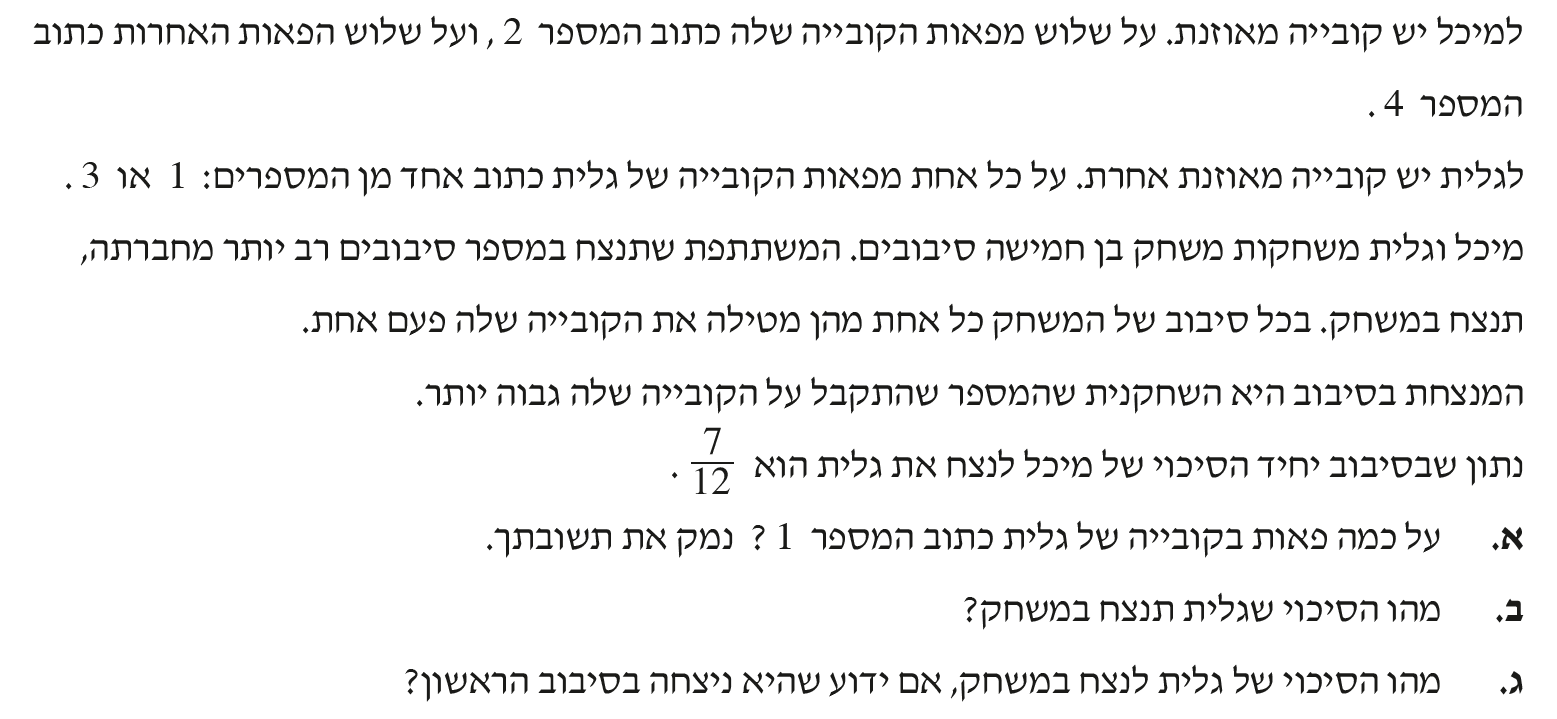
\includegraphics[width=\textwidth]{winter-2018-3}
\end{center}

\textbf{סעיף א}

נסמן ב-%
$n$
את המספר הפאות של הקוביה של גלית שכתוב עליהן
$1$.
מאורע אחד הוא שמיכל תנצח כי היא מטילה 
$4$
בהסתברות
$\frac{3}{6}$
לא משנה מה גלית מטילה. מאורע שני הוא שמיכל תנצח כי היא מטילה 
$2$
בהסתברות
$\frac{3}{6}$
וגלית מטילה
$1$
בהסתברות
$\frac{n}{6}$.
המאורעות זרים זה לזה ולכן:
\begin{eqnarray*}
P(\textrm{\R{מיכל תנצח}}) &=&
\frac{3}{6}\cdot 1 + \frac{3}{6}\cdot \frac{n}{6}=\frac{7}{12}\\
n &=& 1\,.
\end{eqnarray*}
\textbf{סעיף ב}

גלית תנצח אם היא תנצח ב-%
$3,4,5$
סיבובים. נשמתמש בנוסחת ברנולי כדי לקבל את ההסתברות כתלות של ההסתברות של גלית לנצח בסיבוב אחד שהיא המשלים להסתברות שמיכל תנצח
$1-\frac{7}{12}=\frac{5}{12}$:
\[
P(\textrm{\R{גלית תנצח}})={5\choose 3}\left(\frac{5}{12}\right)^3\left(\frac{7}{12}\right)^2+{5\choose 4}\left(\frac{5}{12}\right)^4\left(\frac{7}{12}\right)^1+{5\choose 5}\left(\frac{5}{12}\right)^5\left(\frac{7}{12}\right)^0=0.3466\,.
\]
\textbf{סעיף ג}

הניסוח
\textbf{אם ידוע}
מכוון להסתברות מותנית. נסמן ב-%
$G$
את המאורע שגלית תנצח במשחק וב-%
$R$
את המאורע שהיא תנצח בסיבוב הראשון:
\[
P(G/R) = \frac{P(G \cap R)}{P(R)}\,.
\]
כדי שגלית תנצח במשחק וגם בסיבוב הראשון, היא חייבת לנצח בסיבוב הראשון וגם ב-%
$2$
או
$3$
או
$4$
מהסיבובים הנותרים:
\begin{eqnarray*}
P(G \cap R)&=&\frac{5}{12}\left[{4 \choose 4}\left(\frac{5}{12}\right)^4 \left(\frac{7}{12}\right)^0+
{4 \choose 3}\left(\frac{5}{12}\right)^3 \left(\frac{7}{12}\right)^1+
{4 \choose 2}\left(\frac{5}{12}\right)^2 \left(\frac{7}{12}\right)^2\right]\\
&=&\textstyle\frac{5}{12}\cdot 0.5534\,.
\end{eqnarray*}
כבר חישבנו ש-%
$P(R)=\frac{5}{12}$
ולכן 
$P(G/R)= 0.5534$.

% !TeX root = probability.tex

%%%%%%%%%%%%%%%%%%%%%%%%%%%%%%%%%%%%%%%%%%%%%%%%%%%%%%%%%%%%%

\selectlanguage{hebrew}

\section{קיץ תשע"ז מועד ב}

\begin{center}
\selectlanguage{english}

\includegraphics[width=.95\textwidth]{summer-2017b-3}
\end{center}
הניסוח "מוציאים באקראי
$\ldots$
\textbf{ולאחר מכן}
שוב מוציאים באקראי" מכוונן לשימוש בעץ. נסמן ב-%
$b$
את מספר הכדורים הכחולים בקופסה
\L{I}.
בתרשים (בעמוד הבא) בכל צומת רשום שני זוגות של מספרים: למעלה רשום מספר הכדורים האדומים ומספר הכדורים הכחולים בקופסה
\L{I}
ומתחתיו מספר הכדורים האדומים ומספר הכדורים הכחולים בקופסה
\L{II}.
על הקשתות רשום צבע הכדור שנשלף ומתחתיו ההסתברות לשלוף את הצבע. למשל, בקשת הראשונה נשלף כדור אדום וההסתברות היא מספר הכדורים האדומים 
$10-b$
חלקי מספר הכדורים בקופסה
$(10-b)+b=10$.

\begin{figure}
\begin{center}
\begin{tikzpicture}
[grow=right,
level 1/.append style={text width=2cm,level distance=5cm,sibling distance=10em},
level 2/.append style={text width=2cm,level distance=7cm,sibling distance=6em}]
\node[text width=2cm] {(10-b,b)\\(3,7)} % root
child {
  node {(10-b,b)\\(3,7)}
    child {
      node {(10-b,b)\\(3,7)}
      edge from parent node[below] {\R{כחול}}
        node[above,xshift=16mm,yshift=-2mm] {$\frac{b}{10}$}
    }
    child {
      node {(9-b,b)\ *\\(4,7)}
      edge from parent node[above] {\R{אדום}}
        node[below,xshift=16mm,yshift=2mm] {$\frac{10-b}{10}$}
    }
    edge from parent node[below] {\R{כחול}} node[above,xshift=8mm,yshift=0mm] {$\frac{b}{10}$}
}
child { 
  node {(9-b,b)\\(4,7)}
    child {
      node {(9-b,b)\ *\\(4,7)}
      edge from parent node[below] {\R{כחול}}
        node[above,xshift=16mm,yshift=-2mm] {$\frac{b}{9}$}
    }
    child {
      node {(8-b,b)\\(5,7)}
      edge from parent node[above] {\R{אדום}}
        node[below,xshift=16mm,yshift=2mm] {$\frac{9-b}{9}$}
    }
    edge from parent node[above] {\R{אדום}} 
      node[below,xshift=8mm,yshift=0mm] {$\frac{10-b}{10}$}
};
\end{tikzpicture}
\end{center}
\end{figure}

\textbf{סעיף א}

הכוכביות בתרשים מסמנות את שני המסלולים המגיעים למאורע המבוקש 
$R1$:
שנשלף כדור אדום אחד בדיוק מקופסה
\L{I}.
שתי השליפות הן זרות זו לזו ולכן ההסתברות היא סכום ההסתברות לאורך כל אחד מהמסלולים, והסתברות זו נתונה בשאלה:
\[
P(R1)=\frac{10-b}{10}\cdot\frac{b}{9} + \frac{b}{10}\cdot\frac{10-b}{10} = \frac{19}{36}\,.
\]
נפשט ונקבל משוואה ריבועית 
$b^2-10b+25=0$
שיש לה פתרון אחד
$b=5$.


\textbf{סעיף ב}

מהמידע הרשום בצד הימיני של התרשים אפשר לראות שמספר הכדורים האדומים שנמצאים בקופסה
\L{II}
הם:
$5,4,4,7$.
נסכם את ההסתברויות של המאורע
$P(R2$,
לשלוף כדור אדום מקופסה
\L{II},
לאורך כל אחד מהמסלולים כאשר קודם נציב 
$b=5$
שמצאנו לעיל:
\[
\begin{array}{rcl}
P(R2)&=&\displaystyle\left(\frac{5}{10}\cdot\frac{4}{9}\right)\left(\frac{5}{12}\right)+
\left(\frac{5}{10}\cdot\frac{5}{9}\right)\left(\frac{4}{11}\right)+\\
&&\displaystyle\left(\frac{5}{10}\cdot\frac{5}{10}\right)\left(\frac{4}{11}\right)+
\left(\frac{5}{10}\cdot\frac{5}{10}\right)\left(\frac{3}{10}\right)
=0.3595\,.
\end{array}
\]

\textbf{סעיף ג}

הניסוח
"\textbf{ידוע ש-}"
מכוון להסתברות מותנית. המאורע החדש הוא
$P(R3)$:
נשארו שלושה כדורים אדומים בקופסה 
\L{II}:
\[
P(R3/R2)=\frac{P(R3\cap R2)}{P(R2)}\,.
\]
את
$P(R2)$
חישבנו בסעיף הקודם.

נשארו שלושה כדורים אדומים רק אם היו אברעה כדורים אדומים לפני הבחירה, מאורע 
$R4$.
ההסתברות 
$P(R4)$
למעשה נתונה
$\frac{19}{36}$,
והיא ההסתברות להגיע לאחד המצבים המסומנים בכוכבית. מכאן שההסתברות של 
$P(R3)$
היא ההסתברות להגיע לאחד מהמצבים כפול ההסתברות לשלוף כדור אדום במצב זה:
\[
P(R3)=P(R4)\cdot \textstyle\frac{4}{11}\,.
\]
ההסתברות המותנית הדרושה היא:
\[
P(R3/R2)=\frac{\frac{19}{36}\cdot\frac{4}{11}}{0.3595}=0.53385\,.
\]

%%%%%%%%%%%%%%%%%%%%%%%%%%%%%%%%%%%%%%%%%%%%%%%%%%%%%%%%%%%%%%%%%%%

\section{קיץ תשע"ז מועד א}

\begin{center}
\selectlanguage{english}
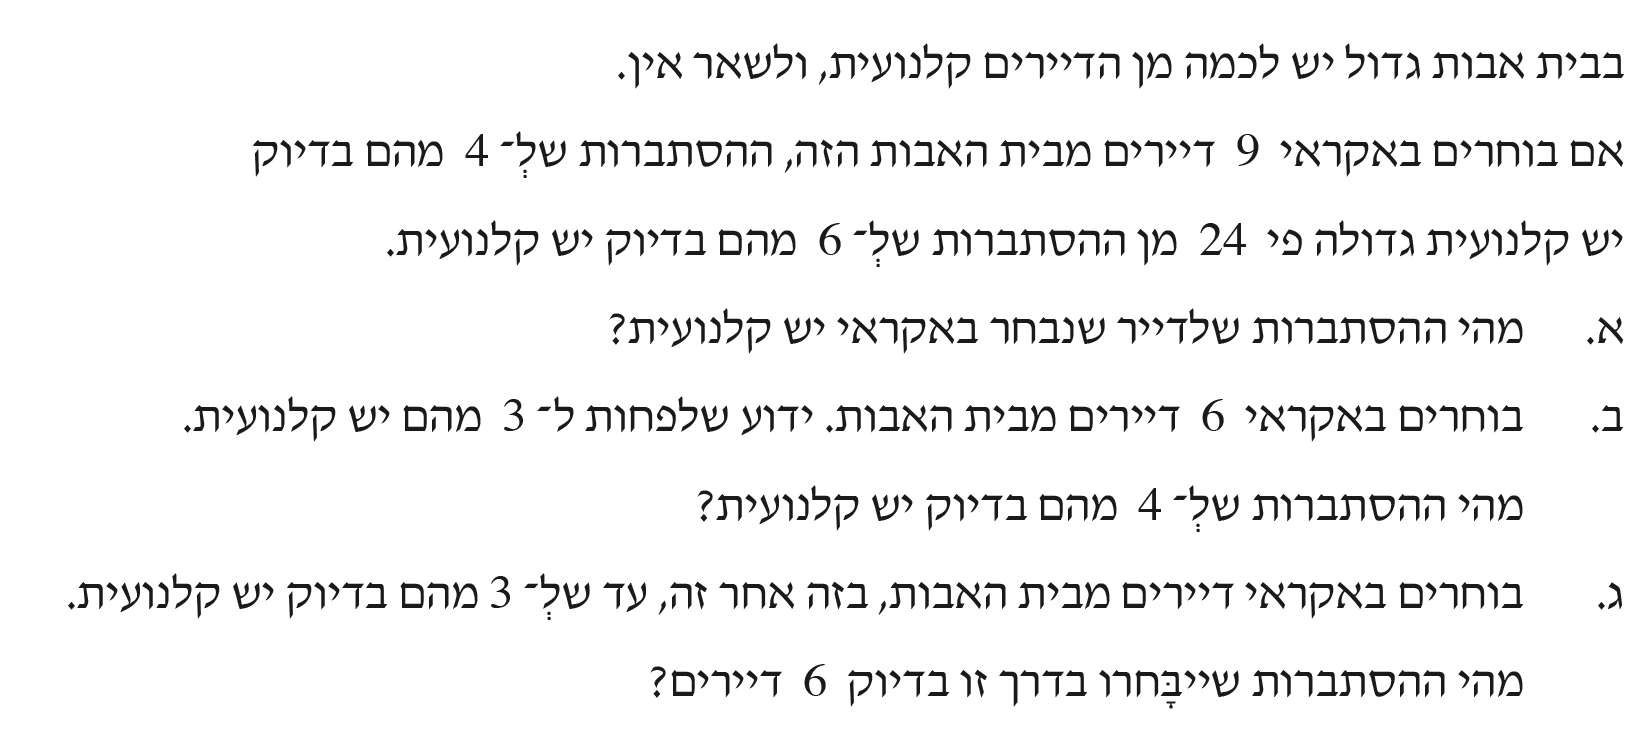
\includegraphics[width=.95\textwidth]{summer-2017a-3}
\end{center}

\textbf{סעיף א}

נסמן ב-%
$D$
את המאורע "לדייר יש קלנועית" ונסמן
$P(D)=p$.
לפי ניסוח השאלה הצלחה היא בחירת דייר עם קלנועית ונמסר מידע על "בדיוק" מספר ההצלחות, ולכן נשמתש בנוסחת ברנולי לכדי לקבל משוואה במשתנה 
$p$:
\begin{eqnarray*}
{9\choose 4} p^4 (1-p)^5&=&24 {9\choose 6} p^6 (1-p)^3\\
\frac{1}{4}(1-p)^2&=&\frac{24}{6}p^2\\
15p^2+2p-1&=&0\\
p&=&\frac{1}{5}=0.2\,,
\end{eqnarray*}
כאשר השורש 
$-\frac{1}{3}$
אינו יכול להיות פתרון כי הסתברות חייבת גדול או שווה לאפס.

\textbf{סעיף ב}

נסמן ב-%
$N$
את המאורע של "מספר הדיירים שיש להם קלנועית". הניסוח
"\textbf{ידוע ש-}"
מכוון להסתברות מותנית:
\[
P(N=4/N\ge3) = \frac{P(N=4\cap N\ge 3)}{P(N\ge 3)}\,.
\]
כאשר קבוצה אחת בחיתוך היא תת-קבוצה של השנייה, אפשר לפשט את החיתוך ולהשתמש רק בקבוצה הקטנה יותר. ברור שאם 
$N$
גדול או שווה ל-%
$3$
\textbf{וגם}
$N$
שווה ל-%
$4$
אז
$N$
שווה ל-%
$4$:
\[
P(N=4/N\ge3) =\frac{P(N=4)}{P(N\ge 3)}\,.
\]
לפי נוסחת ברנולי:
\[
P(N=4)={6\choose 4} 0.2^4 (1-0.2)^2= 0.01536\,.
\]
המונה
$P(N\ge 3)$
אפשר לחשב בשתי דרכים. בצורה ישירה:
\begin{eqnarray*}
P(N\ge 3)&=&{6\choose 3}0.2^3(1-0.2)^3+{6\choose 4}0.2^4(1-0.2)^2+\\
&&{6 \choose 5} 0.2^5(1-0.2)^1+ {6 \choose 6} 0.2^6(1-0.2)^0=0.099\,,
\end{eqnarray*}
או לפי המשלים:
\begin{eqnarray*}
P(N\ge 3)=1-P(N<3)&=&
1-0.2^0(1-0.2)^6-{6\choose 1}0.2^1(1-0.2)^5 -\\
&&{6 \choose 2} 0.2^2(1-0.2)^4=0.099\,.
\end{eqnarray*}
התשובה לשאלה היא:
\[
P(N=4/N\ge3) =\displaystyle\frac{P(N=4)}{P(N\ge 3)}=\displaystyle\frac{0.01536}{0.099}=0.15534\,.
\]
\textbf{סעיף ג}

הניסוח 
"\textbf{עד ש}"
אומר שהבחירה 
\textbf{האחרונה} 
תהיה "הצלחה" ושיהיו שתי "הצלחות" בחמשת הבחירות הקודמות. נסמן הצלחה ב-%
$+$
וכישלון ב-%
$-$
ונסדר את הדרישה בשאלה בשורה:
\[
\overbrace{\pm\;\pm\;\pm\;\pm\;\pm}^{2/5}\quad\quad \overbrace{+}^{1/1}
\]
התשובה מתקבלת מנוסחת ברנולי לבחירות הראשונות כפול ההסתברות
$p$
לבחירה האחרונה:
\[
\left[{5\choose 2}0.2^2 (1-.02)^3\right]\cdot 0.2=0.04096\,.
\]

%%%%%%%%%%%%%%%%%%%%%%%%%%%%%%%%%%%%%%%%%%%%%%%%%%%%%%%%%%%%%

\section{חורף תשע"ז}

\begin{center}
\selectlanguage{english}
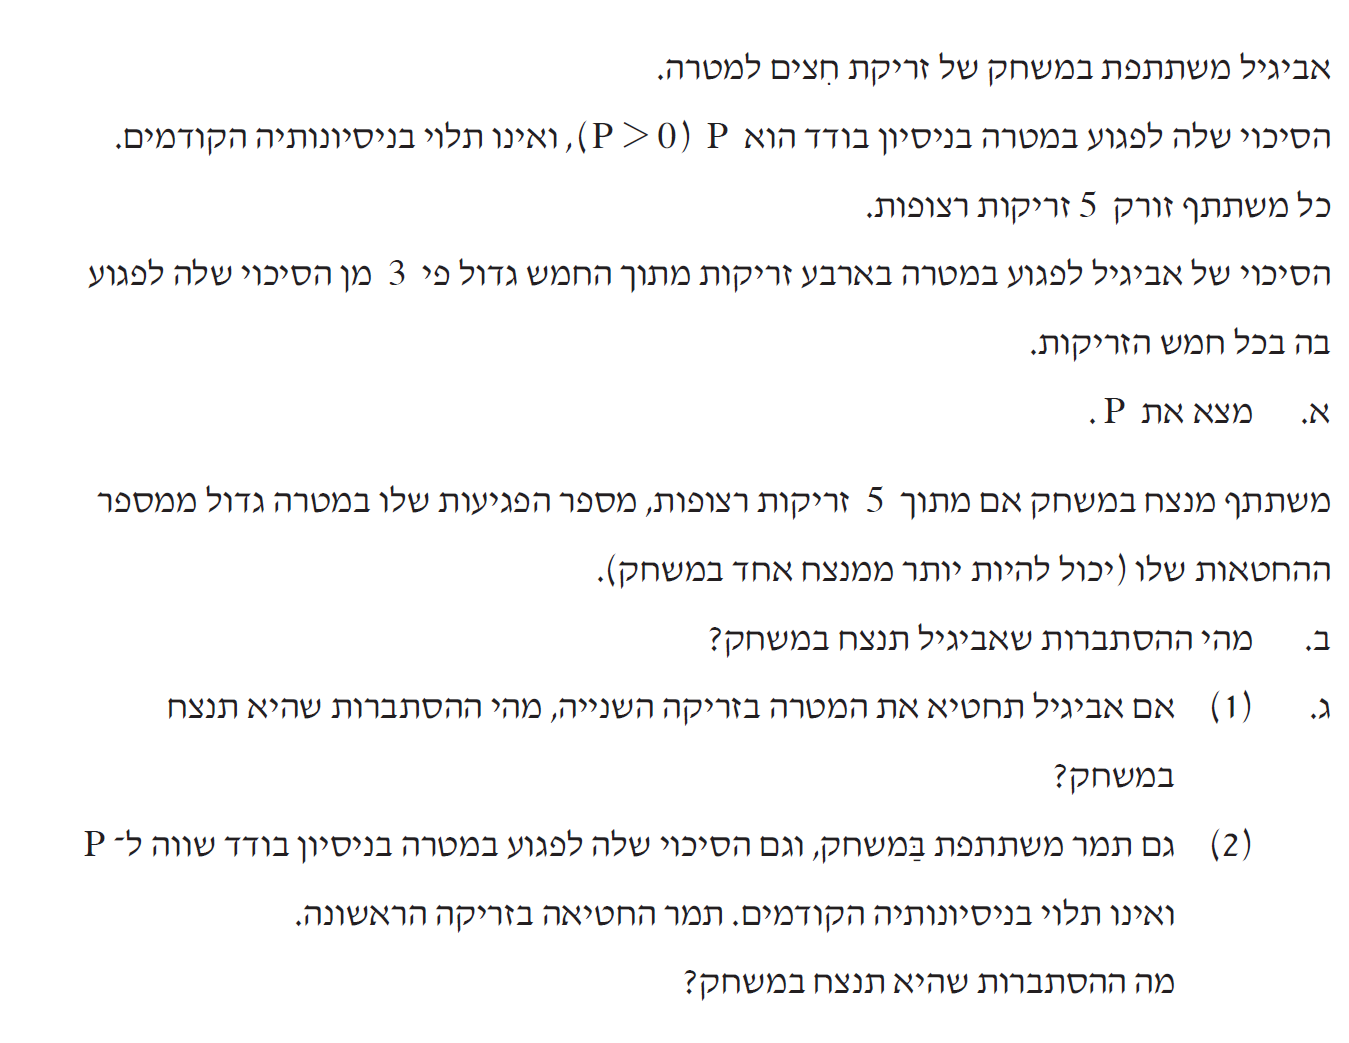
\includegraphics[width=.95\textwidth]{winter-2017-3.png}
\end{center}

\textbf{סעיף א}

נסמן ב-%
$A$
את המאורע "אביגיל פוגעת" ונסמן
$P(A)=p$.
לפי ניסוח השאלה הצלחה היא פגיעה במטרה ונמסר מידע על מספר ההצלחות, ולכן נשמתש בנוסחת ברנולי לכדי לקבל משוואה במשתנה 
$p$:
\begin{eqnarray*}
{5 \choose 4} p^4(1-p)^1 &=& 3{5\choose 5}p^5(1-p)^0\\
5(1-p) &=& 3p\\
p&=&\frac{5}{8}\,.
\end{eqnarray*}

\textbf{סעיף ב}

נסמן ב-%
$N5$
את מספר הפגיעות של אביגיל מתוך חמש זריקות. ניצחון שלה היא 
$N5\geq 3$
וההסתברות היא:
\[
P(N5\geq 3)=
{5 \choose 3}p^3(1-p)^2 + {5 \choose 4}p^4(1-p)^1 + {5 \choose 5}p^5(1-p)^0.
\]
נציב
$p=\displaystyle\frac{5}{8}$
ונקבל
$0.7248$.

\textbf{סעיף ג (1)}

לדעתי ניסוח השאלה לא ברור. אני פירשתי אותה כך: מה ההסתברות של
\textbf{המאורע}
"אביגיל מחטיאה בזריקה השנייה ופוגעת בשלוש או ארבע מהזריקות האחרות"? כותב הבחינה התכוון להסתברות מותנית: "%
\textbf{אם ידוע}
שאביגיל החטיאה בזריקה השנייה, מה ההסתברות שהיא פוגעת בשלוש או ארבע מהזריקות האחרות"?

נסמן ב-%
$T2$
את המאורע שאביגיל מחטיאה בזריקה השנייה, ונסמן ב-%
$N4$
את מספר הפגיעות שלה מתוך ארבע זריקות. ההסתברות המותנית היא:
\[
P(N4\geq 3/T2) = \frac{P(N4\geq 3\cap T2)}{P(T2)}\,.
\]
הזריקות לא תלויות אחת בשנייה ולכן:
\[
P(N4\geq 3/T2) = \frac{P(N4\geq 3)\cdot P(T2)}{P(T2)}=P(N4\geq 3)\,,
\]
ולפי נוסחת ברנולי:
\[
P(N4\geq 3/T2) =P(N4\geq 3)=
{4\choose 4}\left(\frac{5}{8}\right)^4 \left(\frac{3}{6}\right)^0 +{4\choose 3}\left(\frac{5}{8}\right)^3\left(\frac{3}{8}\right)^1 = 0.5188\,.
\]

\textbf{סעיף ג (2)}

ההסתברות של תמר לפגוע זהה להסתברות של אביגיל לפגוע ולכן ניתן להשמתמש בתוצאות שכבר חישבנו. גם לא משנה איזו זריקה החטיאה כי הזריקות בלתי תלויות, ולכן לפי סעיף ג (1) ההסתברות של תמר לנצח היא גם
$0.5188$.

% !TeX root = probability.tex

%%%%%%%%%%%%%%%%%%%%%%%%%%%%%%%%%%%%%%%%%%%%%%%%%%%%%%%%%%%%%

\section{קיץ תשע"ו מועד ב}

\begin{center}
\selectlanguage{english}
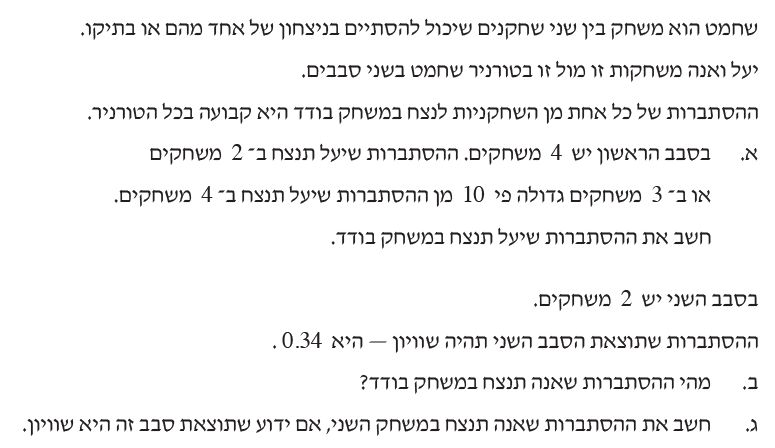
\includegraphics[width=.86\textwidth]{summer-2016b-3}
\end{center}

\textbf{סעיף א}

נסמן את המאורע "יעל תנצח במשחק בודד" ב-%
$Y$ \L{(Yael)}
ונסמן
$y=P(Y)$.
הצלחה מוגדרת על ידי ניצחונות של יעל והשאלה מספקת מידע על מספרי ההצלחות ולכן נשמתמש בנוסחת ברנולי:
\begin{eqnarray*}
{4 \choose 2}y^2(1-y)^2 + {4\choose 3}y^3(1-y) &=& 10\cdot {4\choose 4}y^4(1-y)^0\\
8y^2+8y-6&=&0\\
y&=&\frac{1}{2}\,,
\end{eqnarray*}
ונתעלם מהשורש השני 
$-\frac{3}{2}$
כי הסתברות לא יכולה להיות שלילי.

\textbf{סעיף ב}

נסמן את המאורע "אנה תנצח במשחק בודד" ב-%
$A$ \L{(Anna)}
ונסמן
$a=P(A)$.

נסמן ב-%
$S$ \L{(shivyon)}
את המאורע שתוצאת הסבב השני תהיה תיקו. האפשרויות לקבל שוויון הן ניצחון אחד לאנה וליעל בהסתברות 
$ya+ay$,
או תיקו בשני המשחקים בהסתברות
$(1-(y+a))^2$
כי ההסתברות לתיקו במשחק אחד היא המשלים לסכום ההסתברויות שאחת מהן תנצח. נציב
$y=\frac{1}{2}$
והמידע ש-%
$P(S)=0.34$
ונקבל:
\begin{eqnarray*}
{2 \choose 1}ya + (1-(y+a))^2 &=&P(S)= 0.34\\
a + (\textstyle\frac{1}{2}-a)^2&=&0.34\\
a&=&0.3\,,
\end{eqnarray*}
כאשר נתעלם מהשורש
$-0.3$
כי הסתברות לא יכולה להיות שלילית.

\textbf{סעיף ג}

נסמן את המאורע "אנה תנצח במשחק השני" ב-%
$A2$.

הניסוח
"\textbf{אם ידוע ש-}"
מכוון להסתברות מותנית:
\begin{eqnarray*}
P(A2/S) &=& \frac{P(A2\:\cap\;S)}{P(S)}\\
&=&\frac{ya}{P(S)}=\frac{0.5\cdot 0.3}{0.34}=0.4412\,.
\end{eqnarray*}

ההסתברות לשיוון בסבב השני נתונה. אם אנה תנצח במשחק השני, יהיה שוויון רק אם גם יעל תנצח במשחק הראשון:
\[
\frac{ya}{.34}=\frac{0.5\cdot 0.3}{.34}=0.4412\,.
\]
שימו לב שאם יש שיוון ואנה מנצחת במשחק הראשון, יעל חייבת לנצח במשחק הראשון ולכם המנה היא 
$ya$.

%%%%%%%%%%%%%%%%%%%%%%%%%%%%%%%%%%%%%%%%%%%%%%%%%%%%%%%%%%%%%%

\newpage

\section{קיץ תשע"ו מועד א}

\begin{center}
\selectlanguage{english}
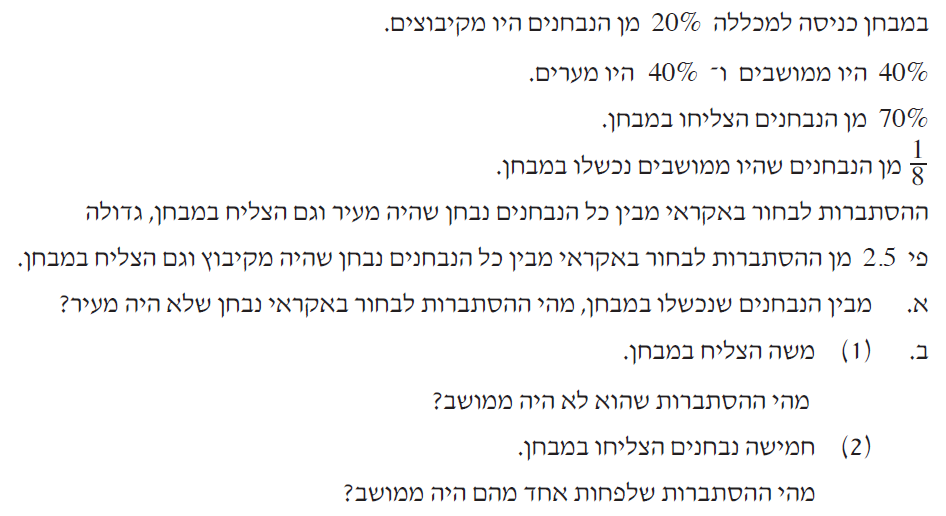
\includegraphics[width=.95\textwidth]{summer-2016a-3}
\end{center}

נסמן את המאורעות השונים בשאלה.
\begin{itemize}
\item $S$ \L{(success)}
הנבחנים שהצליחו.
\item $K$ \L{(kibbutz)} 
נבחנים מקיבוצים.
\item $M$ \L{(moshav)}
נבחנים ממושבים.
\item $E$ \L{(eer)}
נבחנים מערים.
\end{itemize}
ההסתברויות של המאורעות הללו נתונות:
\[
P(K)=0.20,\;P(M)=0.40,\;P(E)=0.40,\;P(S)=0.70\,.
\]
בשאלה שני סוגים של קבוצות: הצלחת הנבחנים ומקום המגורים של הנבחנים ולכן נשתמש בטבלה:
\begin{center}
\selectlanguage{english}
\begin{tikzpicture}[scale=1.25]
\draw (0,0) grid (4,3);
\node at (3.5,3.3) {$K$};
\node at (2.5,3.3) {$M$};
\node at (1.5,3.3) {$E$};
\node at (4.3,2.5) {$S$};
\node at (4.3,1.5) {$\overline{S}$};

\node at (0.5,2.5) {$0.70$};
\node at (0.5,1.5) {$0.30$};
\node at (0.5,0.5) {$1.0$};

%\node at (1.5,2.5) {$0.25$};
%\node at (1.5,1.5) {$0.15$};
\node at (1.5,0.5) {$0.40$};

%\node at (2.5,2.5) {$0.35$};
%\node at (2.5,1.5) {$0.05$};
\node at (2.5,0.5) {$0.40$};

%\node at (3.5,2.5) {$0.10$};
%\node at (3.5,1.5) {$0.10$};
\node at (3.5,0.5) {$0.20$};
\end{tikzpicture}
\end{center}
מידע נוסף שניתן הוא "%
$\frac{1}{8}$
\textbf{מן הנבחנים}
שהיו ממושבים נכשלו במבחן", כאשר הניסוח מכוון להסתברות מותנית. נחשב:
\begin{eqnarray*}
P(\overline{S}/M)&=&P(\overline{S}\cap M) / P(M)\\
P(\overline{S}\cap M)&=&P(\overline{S}/M)\cdot P(M)=\frac{1}{8}\cdot 0.40=0.05\,.
\end{eqnarray*}
הנתון האחרון מתקבל מהפסקאות "ההסתברות לבחור באקראי
\textbf{מבין כל}
הנבחנים נבחן שהיה ב-%
$\cdots$
\textbf{וגם}
הצליח במבחן". הניסוח מכוון לחיתוך הסתברויות, ולכן הנתון הוא
$P(E\cap S)=2.5\cdot P(K\cap S)$.

נחשב את 
$P(S)=0.70$
על ידי סיכום ההסתברויות של המצליחים במבחן בכל מקום מגורים:
\begin{eqnarray*}
P(S)&=&P(K\cap S)+P(M \cap S) + P(K\cap E)\\
0.70&=&P(K\cap S)+ 0.35 + 2.5\cdot P(K\cap S)\\
P(K\cap S)&=&0.10\\
P(E\cap S)&=&0.25\,.
\end{eqnarray*}
נשלים את הטבלה:
\begin{center}
\selectlanguage{english}
\begin{tikzpicture}[scale=1.25]
\draw (0,0) grid (4,3);
\node at (3.5,3.3) {$K$};
\node at (2.5,3.3) {$M$};
\node at (1.5,3.3) {$E$};
\node at (4.3,2.5) {$S$};
\node at (4.3,1.5) {$\overline{S}$};

\node at (0.5,2.5) {$0.70$};
\node at (0.5,1.5) {$0.30$};
\node at (0.5,0.5) {$1.0$};

\node at (1.5,2.5) {$0.25$};
\node at (1.5,1.5) {$0.15$};
\node at (1.5,0.5) {$0.40$};

\node at (2.5,2.5) {$0.35$};
\node at (2.5,1.5) {$0.05$};
\node at (2.5,0.5) {$0.40$};

\node at (3.5,2.5) {$0.10$};
\node at (3.5,1.5) {$0.10$};
\node at (3.5,0.5) {$0.20$};
\end{tikzpicture}
\end{center}
\textbf{סעיף א}

לפי הנוסחה להסתברות מותנית:
\[
P(\overline{E}/\overline{S})=P((K\cup M)/\overline{S}) = \frac{P(K\cap \overline{S})+P(M\cap \overline{S})}{P(\overline{S})}=\frac{0.10+0.05}{0.30}=\frac{1}{2}\,.
\]
\textbf{(1) סעיף ב}

לפי הנוסחה להסתברות מותנית:
\[
P(\overline{M}/S)=P((K\cup E)/S) = \frac{P(K\cap S)+P(E\cap S)}{P(S)}=\frac{0.10+0.25}{0.70}=\frac{1}{2}\,.
\]
\textbf{(2) סעיף ב}

"לפחות אחד ממושב" הוא המשלים ל-"כולם לא מהמושב" ולפי נוסחת ברנולי:
\[
1-P(\overline{M}/S)^5=1-\left(\frac{1}{2}\right)^2=\frac{31}{32}\,.
\]

%%%%%%%%%%%%%%%%%%%%%%%%%%%%%%%%%%%%%%%%%%%%%%%%%%%%%%%%%%%%

\section{חורף תשע"ו}

\begin{center}
\selectlanguage{english}
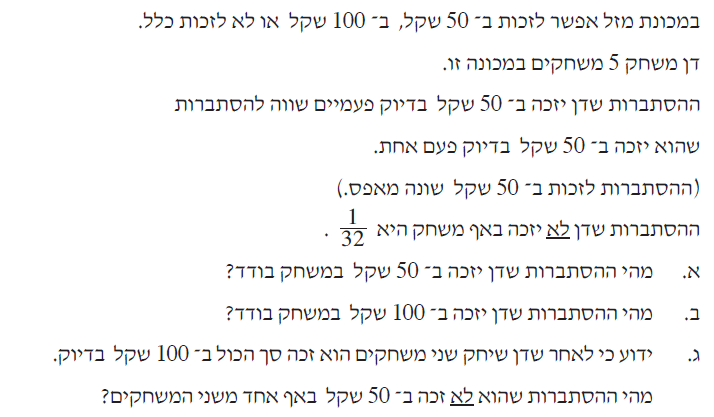
\includegraphics[width=.85\textwidth]{winter-2016-3}
\end{center}

המאורעות הם סכומי הכסף שדן זכה 
$0,50,100$.
נסמן ב-%
$P(n)$
את ההסתברות שדן זכה ב-%
$n$.

\textbf{סעיף א}

הניסוחים "אף אחד" ו-"בדיוק" מכוונים לנוסחת ברנולי. ההסתברות שדן לא זכה (בסכום חיובי) באף אחד מחמישת המשחקים היא 
$P(0)^5=\frac{1}{32}$
ולכן 
$P(0)=\frac{1}{2}$.
לפי המידע הנתון:
\begin{eqnarray*}
{5\choose 2} P(50)^2 (1-P(50))^3 &=& {5\choose 1} P(50) (1-P(50))^4\\
10P(50)&=&5(1-P(50))\\
P(50)&=&\frac{1}{3}\,.
\end{eqnarray*}

\textbf{סעיף ב}

לפי ההסתברות המשלימה:
$P(100) = 1 - P(0) - P(50) = 1-\frac{1}{2}-\frac{1}{3}=\frac{1}{6}$.



\textbf{סעיף ג}

נסמן ב-%
$M2$
את המאורע שדן זכה ב-%
$100$
בשני משחקים ונסמן ב-%
$\overline{50}$
את המאורע שדן לא זכה ב-%
$50$.
הניסוח
"\textbf{ידוע כי}"
מכוון להסתברות מותנית:
\[
P(\overline{50}/M2)=\frac{P(\overline{50}\cap M2)}{P(M2)}
\]
המשחקים מתרחשים אחד אחרי השני ולא לתלויים אחד בשני ולכן ניתן להציג את ההסתברויות בעץ (בעמוד הבא). בסוף כל מסלול רשום המאורעות 
$M2,\overline{50}$
שמתקיימים. ההסתברות המותנית היא:
\[
\frac{\frac{1}{2}\cdot\frac{1}{6} + \frac{1}{6}\cdot \frac{1}{2}}{\frac{1}{2}\cdot\frac{1}{6} + \frac{1}{3}\cdot \frac{1}{3}+ \frac{1}{6}\cdot \frac{1}{2}}  =  \frac{\frac{1}{6}}{\frac{5}{18}}=\frac{3}{5}\,.
\]

\begin{center}
\begin{tikzpicture}
[grow=right,
level 1/.append style={level distance=2cm,
                       sibling distance=7em},
level 2/.append style={level distance=4cm,
                       sibling distance=2.5em}]
\node[left] {$\scriptstyle 0$} % root
child {
  node[right] {$\scriptstyle 100$}
    child {
      node[right] {$\scriptstyle 200\quad \{\overline{50}\}$}
      edge from parent node[below] {$\scriptstyle 1/6$}
    }
    child {
      node[right] {$\scriptstyle 150$}
      edge from parent node[below,near end] {$\scriptstyle 1/3$}
    }
    child {
      node[right] {$\scriptstyle 100\quad \{M2,\overline{50}\}$}
      edge from parent node[above] {$\scriptstyle 1/2$}
    }
    edge from parent node[below,yshift=-2mm] {$\scriptstyle 1/6$}
}
child {
  node[right] {$\scriptstyle 50$}
    child {
      node[right] {$\scriptstyle 150$}
      edge from parent node[below] {$\scriptstyle 1/6$}
    }
    child {
      node[right] {$\scriptstyle 100\quad \{\overline{M2}\}$}
      edge from parent node[below,near end] {$\scriptstyle 1/3$}
    }
    child {
      node[right] {$\scriptstyle 50$}
      edge from parent node[above] {$\scriptstyle 1/2$}
    }
    edge from parent node[below] {$\scriptstyle 1/3$}
}
child {
  node[right] {$\scriptstyle 0$}
    child {
      node[right] {$\scriptstyle 100\quad \{M2,\overline{50}\}$}
      edge from parent node[below] {$\scriptstyle 1/6$}
    }
    child {
      node[right] {$\scriptstyle 50$}
      edge from parent node[below,near end] {$\scriptstyle 1/3$}
    }
    child {
      node[right] {$\scriptstyle 0\quad \{\overline{50}\}$}
      edge from parent node[above] {$\scriptstyle 1/2$}
    }
    edge from parent node[above,yshift=2mm] {$\scriptstyle 1/2$}
}
;
\end{tikzpicture}
\end{center}


% !TeX root = probability.tex

%%%%%%%%%%%%%%%%%%%%%%%%%%%%%%%%%%%%%%%%%%%%%%%%%%%%%%%%%%%%%

%%%%%%%%%%%%%%%%%%%%%%%%%%%%%%%%%%%%%%%%%%%%%%%%%%%%%%%%%%%%%%

\section{קיץ תשע"ה מועד ב}

\begin{center}
\selectlanguage{english}
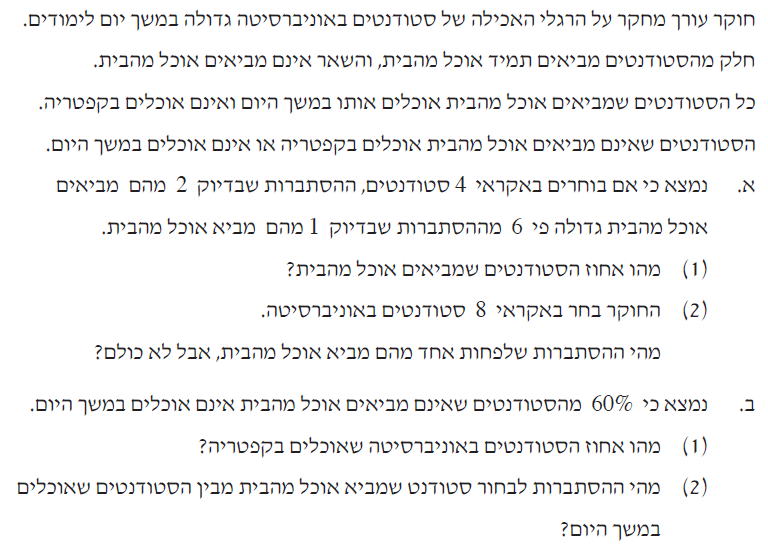
\includegraphics[width=.85\textwidth]{summer-2015b-3}
\end{center}

\textbf{סעיף א (1)}

נסמן את המאורע "מביא אוכל מהבית" ב-%
$M$ \L{mavi}
ונסמן
$b=P(M)$.
המילה "בדיוק" מכוון לנוסחת ברנולי:
\begin{eqn}
{4 \choose 2} b^2(1-b)^2 &=& 6\cdot {4 \choose 1} b (1-b)^3\\
6b&=&24(1-b)\\
b&=&\frac{4}{5}\,.
\end{eqn}
השאלה שואלת על "אחוז" ולכן התשובה היא
$80\%$.

\textbf{סעיף א (2)}

ההסתברות של "לפחות אחד אבל לא כולם" היא המשלים ל-"לא אפס ולא כולם":
\[
1-\left(\frac{1}{5}\right)^8-\left(\frac{4}{5}\right)^8=0.8322\,.
\]

\textbf{סעיף ב (1)}

נסמן את המאורע "אוכל בקפטריה" ב-%
$C$ \L{(cafeteria)}.
בעץ ההסתברויות בעמוד הבא הכוכבית מראה את מהמסלול עבור המאורע 
$C$
ולכן:
\[
P(C)=\frac{1}{5}\cdot \frac{4}{10} = \frac{2}{25}\,.
\]

\begin{figure}
\begin{center}
\begin{tikzpicture}
[grow=right,
level 1/.append style={level distance=3cm,sibling distance=6em},
level 2/.append style={text width=1cm,level distance=4cm,sibling distance=8em}]
\node[text width=1cm] {} % root
child {
  node {}
    edge from parent node[below,xshift=-5mm,yshift=-3mm] {\R{מביא מהבית}}
      node[above,xshift=3mm,yshift=-4pt] {$\frac{4}{5}$}
}
child { 
  node {}
    child {
      node {$*$}
      edge from parent node[below,xshift=5mm,yshift=-3mm] {\R{אוכל בקפטריה}}
        node[above,xshift=11mm,yshift=-2mm] {$\frac{4}{10}$}
    }
    child {
      node {}
      edge from parent node[above,xshift=5mm,yshift=3mm] {\R{לא אוכל}}
        node[below,xshift=10mm,yshift=2mm] {$\frac{6}{10}$}
    }
    edge from parent node[above,xshift=-4mm,yshift=5mm] {\R{לא מביא מהבית}}
      node[below,xshift=4mm,yshift=2mm] {$\frac{1}{5}$}
};
\end{tikzpicture}
\end{center}
\end{figure}
פתרון זה לא כל כך מוצא חן בעיני כי לא ברור מאיפה צץ העץ שבדרך כלל משמש למאורעות סדרתיות כגון הטלת קוביות מספר פעמים. אני מעדיף פתרון מבוסס הסתברות מותנית ואני חושב שניסוח השאלה היתה צריכה להיות "%
\textbf{מבין}
אלה שלא מביאים אוכל
$60\%$
אינם אוכלים בקפטריה". לפי נוסחת ההסתברות השלמה:
\[
P(C) = P(C/M)P(M) + P(C/\overline{M})P(\overline{M})=
0\cdot 0.8 + (1-0.6)\cdot (1-0.8)=0.4\cdot 0.2=0.08\,.
\]


\textbf{סעיף ב (2)}

נסמן ב-%
$O$ \L{(okhel)}
את המאורע "מביא אוכל. המילה
"\textbf{מבין}"
מכוונת להסתברות מותנית, ונחשב אותה תוך שימוש בעובדה ש-%
$M\subseteq O$
ןלכן
$M\cap O = M$:
\begin{eqn}
P(M/O) &=& \frac{P(M \:\cap\: O)}{P(O)}\\
&=& \frac{P(M)}{P(O)}\\
&=&\frac{\frac{4}{5}}{\frac{4}{5}+\frac{2}{25}}=\frac{10}{11}\,.
\end{eqn}

%%%%%%%%%%%%%%%%%%%%%%%%%%%%%%%%%%%%%%%%%%%%%%%%%%%%%%%%%%%%%

\section{קיץ תשע"ה מועד א}

\begin{center}
\selectlanguage{english}
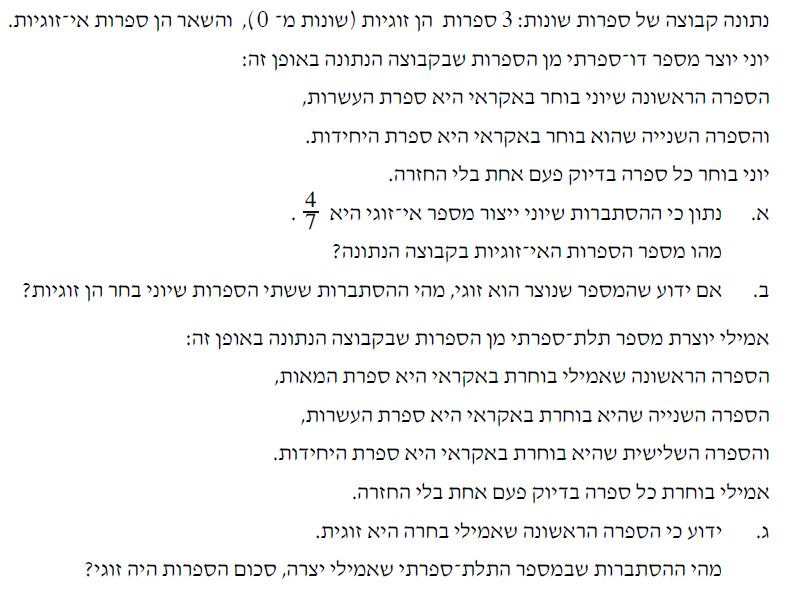
\includegraphics[width=.9\textwidth]{summer-2015a-3}
\end{center}

\textbf{סעיף א}

נסמן את קבוצת הספרות ב-%
$S$ \L{(sifarot)},
קבוצת הספרות הזוגיות ב-%
$Z$ \L{(zugi)},
קבוצת הספרות האי-זוגיות ב-%
$I$ \L{(i-zugi)}.
בחירה של ספרת העשרות ואחר כך ספרת היחידות מכוונת לעץ הסתברויות. במקום לרשום את מספרי הספרות בצמתים וההסתברויות על הקשתות, נפשט את התרשים ונרשום בכל צומת את ההסתברויות שליפת ספרה זוגית או אי-זוגית
$(P(Z=k_1),P(I=k_2))$.

\begin{center}
\begin{tikzpicture}
[grow=right,
level 1/.append style={text width=2cm,level distance=3.5cm,sibling distance=6em},
level 2/.append style={text width=2.5cm,level distance=4.5cm,sibling distance=3.5em}]
\node[text width=2cm] {$\left(\frac{3}{n},\frac{n-3}{n}\right)$} % root
child {
  node {$\left(\frac{3}{n-1},\frac{n-4}{n-1}\right)$}
    child {
      node {$\left(\frac{3}{n-2},\frac{n-5}{n-2}\right)\quad *$}
      edge from parent node[below,xshift=5mm,yshift=-1mm] {\R{אי-זוגי}}
    }
    child {
      node {$\left(\frac{2}{n-2},\frac{n-4}{n-2}\right)$}
      edge from parent node[above,xshift=5mm,yshift=1mm] {\R{זוגי}}
    }
    edge from parent node[below,yshift=-1mm] {\R{אי-זוגי}}
}
child { 
  node {$\left(\frac{2}{n-1},\frac{n-3}{n-1}\right)$}
    child {
      node {$\left(\frac{2}{n-2},\frac{n-4}{n-2}\right)\quad *$}
      edge from parent node[below,xshift=5mm,yshift=-1mm] {\R{אי-זוגי}}
    }
    child {
      node {$\left(\frac{1}{n-2},\frac{n-3}{n-2}\right)$}
      edge from parent node[above,xshift=5mm,yshift=1mm] {\R{זוגי}}
    }
    edge from parent node[above] {\R{זוגי}}
};
\end{tikzpicture}
\end{center}
המאורע
$YI$
שיוני ייצור מספר אי-זוגי יתרחש רק אם הבחירתו השנייה היא ספרה אי-זוגית. המסלולים המתאימים מסומנים בתרשים בכוכביות. נחשב את ההסתברות ונשווה להסתברות הנתונה:
\begin{eqn}
P(YI)&=&\frac{3}{n}\cdot\frac{n-3}{n-1} \;+\; \frac{n-3}{n}\cdot\frac{n-4}{n-1} = \frac{4}{7}\\
4n(n-1)&=&7(n-3)(n-1)\\
n&=&7\\
|I|&=&n-3=4\,.
\end{eqn}
נתון ש-%
$n\geq 3$
ולכן
$n\neq 1$
וניתן לצמצם את 
$n-1$.

\textbf{סעיף ב}

במספר זוגי הספרה האחרונה זוגית. נסמן ב-%
$Z2$
את המאורע ששתי הספרות זוגיות ונסמן ב-%
$ZA$ \L{aharona}
את המאורע ספרה אחרונה זוגית. הניסוח
"\textbf{אם ידוע}"
מכוון להסתברות מותנית:
\begin{eqn}
P(Z2/ZA) &=& \frac{P(Z2\:\cap\:ZA)}{P(ZA)}\\
&=&\frac{P(Z2)}{P(ZA)}\\
&=&\frac{\frac{3}{7}\cdot\frac{2}{6}}{1-\frac{4}{7}}=\frac{1}{3}\,.
\end{eqn}
השתמשנו ב-%
$Z2\subseteq ZA$ 
כי אם שתי הספרות זוגיות אזי הספרה האחרונה זוגית, ובעובדה ש-%
$P(ZA)=1-P(YI)$
שחישבנו בסעיף הקודם. החישוב של
$P(Z2)$
היא ההסתברות שמתקבלת מהמסלול העליון בעץ עבור בחירה של שתי ספרות זוגיות.

\textbf{סעיף ג}

הסכום יהיה זוגי רק אם שתי הספרות האחרונת הן זוגיות או אי-זוגיות:
\begin{eqn}
2k_1+2k_2+2k_3&=&2(k_1+k_2+k_3)\\
2k_1+2(k_2+1)+2(k_3+1)&=&2(k_1+k_2+k_3+1)\,.
\end{eqn}
נסמן ב-%
$Z1$
את המאורע שהספרה הראשונה זוגית ונסמן ב-%
$S$ \L{(sekhum)}
את המאורע שסכום הספרות זוגי. המילה "ידוע" מכוון להסתברות מותנית ולכן:
\begin{eqn}
P(S/Z1)&=& \frac{P(S\:\cap\:Z1)}{P(Z1)}\\
&=& \frac{P(S\:\cap\:Z1)}{P(Z1)}\\
&=&\frac{\frac{3}{7}\cdot\frac{2}{6}\cdot \frac{1}{5}+
\frac{3}{7}\cdot\frac{4}{6}\cdot \frac{3}{5}}
{\frac{3}{7}}=\frac{7}{15}\,.
\end{eqn}
המנה חושב משני המסלולים המסומנים בכוכביות בעץ ההסתברויות בעמוד הבא, כי הם מתחילים עם בחירה של ספרה זוגית ואז שני ואז או שתי ספרות זוגיות או שתי ספרות אי-זוגיות כדי לקבל סכום זוגי.
\begin{center}
\begin{tikzpicture}
[grow=right,
level 1/.append style={level distance=3cm,sibling distance=10em},
level 2/.append style={level distance=3cm,sibling distance=10em},
level 3/.append style={level distance=4cm,sibling distance=5em}]
\node {$\left(\frac{3}{7},\frac{4}{7}\right)$} % root
  child {
    node {$\cdots$}
    edge from parent node[below,yshift=-8pt] {\R{אי-זוגי}}
  }
child {
  node {$\left(\frac{2}{6},\frac{4}{6}\right)$}
child {
  node {$\left(\frac{2}{5},\frac{3}{5}\right)$}
    child {
      node {$\left(\frac{2}{4},\frac{2}{4}\right)\quad *$}
      edge from parent node[below,xshift=5mm,yshift=-2mm] {\R{אי-זוגי}}
    }
    child {
      node {$\left(\frac{1}{4},\frac{3}{4}\right)$}
      edge from parent node[above,xshift=5mm,yshift=2mm] {\R{זוגי}}
    }
    edge from parent node[below,yshift=-3mm] {\R{אי-זוגי}}
}
child { 
  node {$\left(\frac{1}{5},\frac{4}{5}\right)$}
    child {
      node {$\left(\frac{1}{4},\frac{3}{4}\right)$}
      edge from parent node[below,xshift=5mm,yshift=-2mm] {\R{אי-זוגי}}
    }
    child {
      node {$\left(\frac{0}{4},\frac{4}{4}\right)\quad *$}
      edge from parent node[above,xshift=5mm,yshift=2mm] {\R{זוגי}}
    }
    edge from parent node[above,yshift=2mm] {\R{זוגי}}
}
  edge from parent node [above,yshift=8pt] {\R{זוגי}}
};
\end{tikzpicture}
\end{center}

%%%%%%%%%%%%%%%%%%%%%%%%%%%%%%%%%%%%%%%%%%%%%%%%%%%%%%%%%

\newpage

\section{חורף תשע"ה}

\begin{center}
\selectlanguage{english}
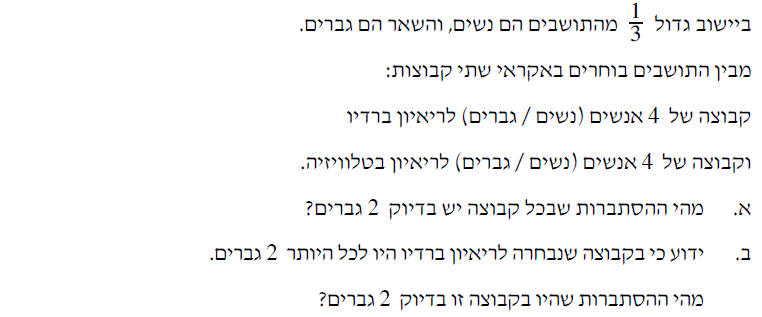
\includegraphics[width=.85\textwidth]{winter-2015-3}
\end{center}

המשמעות של "יישוב גדול" היא (כנראה) שאפשר לבחור את שתי הקבוצות בלי לשנות את ההסתברות של 
$\frac{1}{3}$
במהלך הבחירה, למרות שהבחירה היא ללא החזרה.

\textbf{סעיף א}

נסמן ב-%
$G2$
את המאורע של בחירת שני בגברים בקבוצה אחת ונסמן ב-%
$G22$
את המאורע של בחירת שני גברים בשתי הקבוצות. בחירת גבר נקראת הצלחה ולכן נשתמש בנוסחת ברנולי כדי לקבל את ההסתברות
\textbf{לבדיוק}
שתי הצלחות בקבוצה אחת:
\[
P(G2)={4 \choose 2}\left(\frac{2}{3}\right)^2\left(1-\frac{2}{3}\right)^2=\frac{8}{27}\,.
\]
לפי ההנחה שאין שינוי בהסתברות של הבחירה בין שתי הקבוצות, נקבל:
\[
P(G22)=P(G2)\cdot P(G2)=\frac{64}{729}\,.
\]

\textbf{סעיף ב}

נסמן את המאורע "לכל היותר שני גברים" ב-%
$G012$.
הניסוח
"\textbf{ידוע כי}"
מכוון להסתברות מותנית:
\begin{eqn}
P(G2/G012)&=&\frac{P(G2 \:\cap\: G012)}{P(G012)}\\
\end{eqn}
$G2\subseteq G012$
ולכן המנה היא
$G2=\frac{8}{27}$.
"לכל היותר שני גברים" הוא הסכום של שלוש נוסחאות ברנולי:
\[
\left(\frac{2}{3}\right)^0\left(\frac{1}{3}\right)^4 + {4\choose 1}\left(\frac{2}{3}\right)^1\left(\frac{1}{3}\right)^3 + {4\choose 2}\left(\frac{2}{3}\right)^2\left(\frac{1}{3}\right)^2=\frac{11}{27}\,
\]
והתשובה לשאלה היא:
\[
P(G2/G012)=\frac{\frac{8}{27}}{\frac{11}{27}}=\frac{8}{11}\,.
\]


% !TeX root = probability.tex

%%%%%%%%%%%%%%%%%%%%%%%%%%%%%%%%%%%%%%%%%%%%%%%%%%%%%%%%%%%%%

\section{קיץ תשע"ד מועד ב}

\begin{center}
\selectlanguage{english}
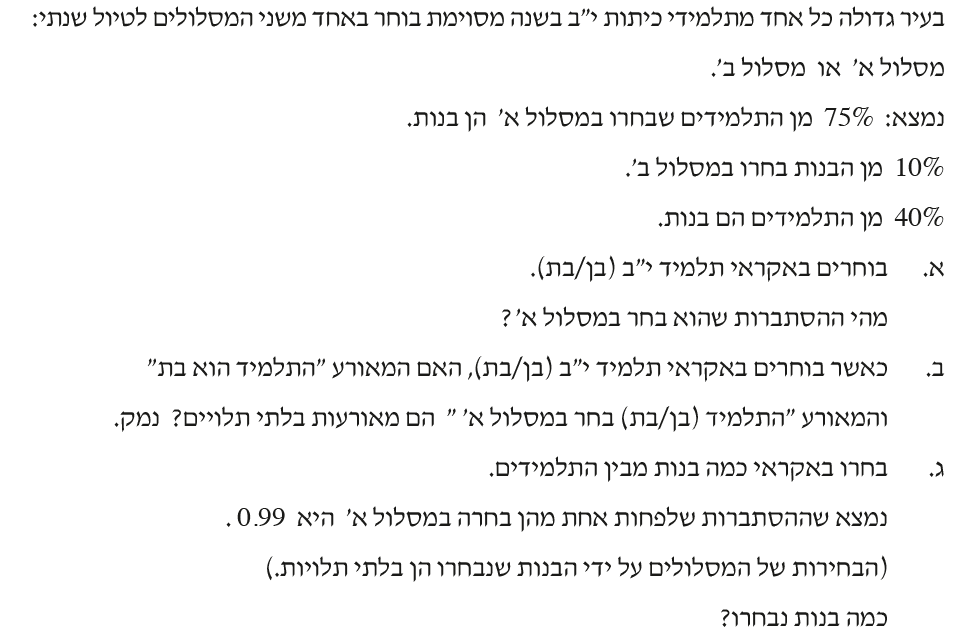
\includegraphics[width=.95\textwidth]{summer-2014b-3}
\end{center}

נמסן את הקבוצות בשאלה:
$G$ \L{(girl)}, $B$ \L{(boy)},
$MA$ \L{(maslul aleph)}, $MB$ \L{(maslul bet)}.
בגלל שיש שני זוגות של קבוצות נציג את ההסתברויות בטבלה. את הטבלה נמלא בשתי דרכים שונות, תחילה ישירות מהנתונים ואחר כך תוך שימוש בהסתברות מותנית.
\begin{center}
\selectlanguage{english}
\begin{tikzpicture}[scale=1.4]
\draw (0,0) grid (3,3);
\node at (2.5,3.3) {$G$};
\node at (1.5,3.3) {$B$};
\node at (3.6,2.5) {$MA$};
\node at (3.6,1.5) {$MB$};
%\node at (2.5,2.7) {$.4-.04=$};
\node at (2.5,2.5) {$.36$};
%\node at (0.5,2.7) {$.36/.75=$};
\node at (0.5,2.5) {$.48$};
%\node at (1.5,2.7) {$.48-.36=$};
\node at (1.5,2.5) {$.12$};
%\node at (0.5,1.7) {$1-.48=$};
\node at (0.5,1.5) {$.52$};
\node at (0.5,0.5) {$1$};
%\node at (1.5,0.7) {$1-.4=$};
\node at (1.5,0.5) {$.60$};
%\node at (2.5,0.7) {\bfseries \R{נתון}};
\node at (2.5,0.5) {$0.40$};
%\node at (1.5,1.7) {$.52-.04=$};
\node at (1.5,1.5) {$.48$};
%\node at (2.5,1.7) {$.1\times .4=$};
\node at (2.5,1.5) {$.04$};
\end{tikzpicture}
\end{center}

\textbf{דרך א'}

נתון ש-% 
$P(G)=0.40$
ונתון ש-%
$10\%$
מהם בחרו במסלול ב', ולכן 
$P(G\cap MB)= .04$,
ומהסתברות משלימה
$P(G\cap MA)= .36$.
הנתון האחרון הוא ש-%
$0.75 P(MA) = 0.36$
ולכן 
$P(MA)=0.36/0.75=0.48$.
את שאר התאים ניתן למלא מהסתברויות משלימות.

\textbf{דרך ב'}

שוב נמלא את התא הימני למטה ב-%
$P(G)=0.40$.
נמשיך:
\begin{eqnarray*}
P(MB/G) &=& \frac{P(MB \:\cap\: G)}{P(G)}=0.10\\
P(MB \:\cap\: G) &=& P(G)P(MB/G) = 0.40\cdot 0.10 = 0.04\,.
\end{eqnarray*}
עוד הסתברות מותנית:
\begin{eqnarray*}
P(G/MA) &=& \frac{P(G \:\cap\: MA)}{P(MA)}=0.75\\
P(MA) &=& \frac{P(G \:\cap\: MA)}{P(G/MA)}=\frac{0.36}{0.75}=0.48\,,
\end{eqnarray*}
ונמלא את שאר התאים באמצעות הסתברויות משלימות.

\textbf{סעיף א}

$P(MA)=0.48$.

\textbf{סעיף ב}
\begin{eqnarray*}
P(G\cap MA) &=&0.36\\
P(G)P(MA)&=&0.40\cdot 0.48=0.19\,.
\end{eqnarray*}
$0.36\neq 0.19$
ולכן המאורעות אינם בלתי תלויים.

\textbf{סעיף ג}

ניתן לחשב "לפחות אחת" על ידי חישוב הסתברות של "אף אחת". ההסתברות שבת לא תבחר מסלול א' היא ההסתברות שהיא תבחר מסלול ב':
\begin{eqnarray*}
P(MB/G) &=& \frac{P(MB \:\cap\: G}{P(G)}= \frac{0.04}{0.40}=0.10\\
(0.10)^n&=&1-0.99=0.01\\
n&=&2\,.
\end{eqnarray*}

%%%%%%%%%%%%%%%%%%%%%%%%%%%%%%%%%%%%%%%%%%%%%%%%%%%%%%%%%%%%%%%%%%%

\section{קיץ תשע"ד מועד א}

\begin{center}
\selectlanguage{english}
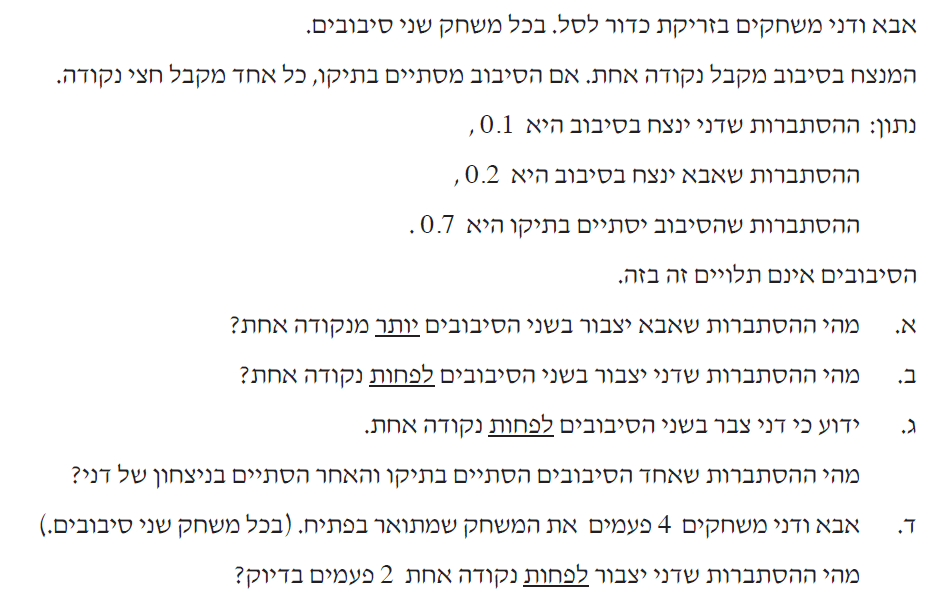
\includegraphics[width=.9\textwidth]{summer-2014a-3}
\end{center}

נסמן ב-%
$D1, D2$ \L{(dani)}
את המאורע שדני מנצח בסיבוב אחד או שניים, נסמן ב-%
$A1, A2$ \L{(abba)}
את המאורע שאבא מנצח בסיבוב אחד או שניים, ונסמן ב-%
$T1, T2$ \L{(teku)}
את המאורע שיהיה תיקו בסיבוב אחד או שניים. השאלה שואלת על סדרה של שני סבבים וזה מכוון לעץ הסתברויות (בעמוד הבא). בסוף כל מסלול רשום מספר הנקודות שאבא צבר ומספר הנקודות שדני צבר.

\begin{figure}
\begin{center}
\selectlanguage{english}
\begin{tikzpicture}
[align=left,grow=right,
level 1/.append style={level distance=3cm,sibling distance=9em},
level 2/.append style={level distance=4cm,
                       sibling distance=3.5em}]
\node[left] {$0$} % root
child {
  node[right] {$\frac{1}{2}$}
    child {
      node[below right,xshift=10pt,yshift=4pt] {$(i) A2=1,D2=1$}
      edge from parent node[below,yshift=-1mm] {$0.7$}
    }
    child {
      node[right,xshift=10pt] 
        {$(h) A2=\frac{1}{2},D2=\frac{1}{2}$}
      edge from parent node[below,xshift=4mm] {$0.1$}
    }
    child {
      node[right,xshift=10pt] 
        {$(g) A2=1\frac{1}{2},D2=\frac{1}{2}$}
      edge from parent node[above,yshift=1mm] {$0.2$}
    }
    edge from parent 
      node[below,xshift=-4mm,yshift=-3mm] {\R{תיקו} $0.7$}
}
child {
  node[right] {$0$}
    child {
      node[right,xshift=10pt] 
        {$(f) A2=\frac{1}{2},D2=1\frac{1}{2}$}
      edge from parent node[below,yshift=-1mm] {$0.7$}
    }
    child {
      node[right,xshift=10pt] {$(e) A2=0,D2=2$}
      edge from parent node[below,xshift=4mm] {$0.1$}
    }
    child {
      node[right,xshift=10pt] {$(d) A2=1,D2=1$}
      edge from parent node[above,yshift=1mm] {$0.2$}
    }
    edge from parent 
      node[below] {\R{דני} $0.1$}
}
child {
  node[right] {$1$}
    child {
      node[right,xshift=10pt] {$(c) A2=1\frac{1}{2},D2=\frac{1}{2}$}
      edge from parent node[below,yshift=-1mm] {$0.7$}
    }
    child {
      node[right,xshift=10pt] {$(b) A2=1,D2=1$}
      edge from parent node[below,xshift=4mm] {$0.1$}
    }
    child {
      node[above right,xshift=10pt] {$(a) A2=2, D2=0$}
      edge from parent node[above,yshift=1mm] {$0.2$}
    }
    edge from parent
       node[above,xshift=-4mm,yshift=3mm] {\R{אבא} $0.2$}
};
\end{tikzpicture}
\end{center}
\end{figure}

\textbf{סעיף א}

במסלול בהם אבא צובר יותר מנקודה אחת הם
\L{(a), (c), (g)},
וההסתברות היא:
\[
P(A2>1)=0.2\cdot 0.2 \,+\, 0.2\cdot 0.7 \,+\, 0.7\cdot 0.2 \,=\,0.32\,.
\]


\textbf{סעיף ב}

המסלולים בהם דני צבר לפחות נקודה אחת הם
\L{(b), (d), (e), (f), (h), (i)}
וההסתברות היא:
\[
P(D2\geq 1)=0.2\cdot 0.1 \,+\,0.1\cdot 0.2 \,+\, 0.1\cdot 0.1 \,+\,0.1\cdot 0.7 \,+\, 0.7\cdot 0.1\,+\,0.7\cdot 0.7\,=\,0.68\,.
\]


\textbf{סעיף ג}

הניסוח "ידוע" מכוון להסתברות מותנית, אבל
$D1\cup T1\subseteq D2\geq 1$
ולכן:
\begin{eqnarray*}
P((D1\cup T1)/D2\geq 1)&=&\frac{P((D1\cup T1) \:\cap\: D2\geq 1)}
  {D2\geq 1}\\
  &=&\frac{P(D1\cup T1)}{D2\geq 1}\\
\frac{0.1\cdot 0.7 \,+\, 0.7\cdot 0.1}{0.68} &=& \frac{7}{34}= 0.2059\,,  
\end{eqnarray*}
כי המסלולים המתאימים הם 
\L{(f), (h)}.

\textbf{סעיף ד}

נשמתמש בנוסחת ברנולי כי למצוא את ההסתברות לבדיוק פעמיים:
\[
{4\choose 2}P(D2)^2\: (1-P(D2)^2 =
{4\choose 2} (0.32)^2 (0.68)^2= 0.2841\,.
\]

%%%%%%%%%%%%%%%%%%%%%%%%%%%%%%%%%%%%%%%%%%%%%%%%%%%%%%%%

\section{חורף תשע"ד}

\begin{center}
\selectlanguage{english}
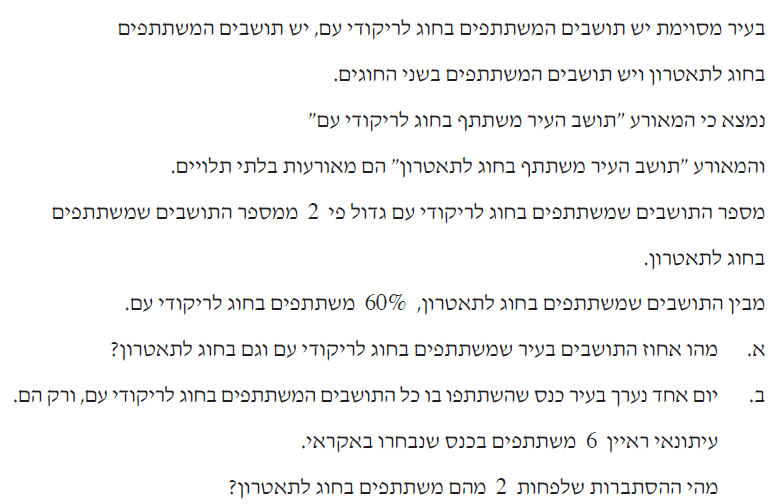
\includegraphics[width=.9\textwidth]{winter-2014-3}
\end{center}

נסמן ב-%
$T$ \L{(theatron)}
את המשתתפים בתאטרון ונסמן ב-%
$R$ \L{(rikudei)}
את המשתתפים בריקודי עם. המילה "מבין" מכוונת להתסברות מותנית. ההסתברויות הן של זוגות של מאורעות ולכן נשתמש בטבלה.


נתון
$P(R/T)=0.6$
ושהאירועים בלתי תלויים. נחשב:
\[
P(R/T)=\frac{P(R\cap T)}{P(T)}=\frac{P(R)\cdot P(T)}{P(T)}=P(R)=0.06\,.
\]
ביחד עם הנתון
$P(R)=2P(T)$
נתחיל למלא את הטבלה:
\begin{center}
\selectlanguage{english}
\begin{tikzpicture}[scale=1.4]
\draw (0,0) grid (3,3);
\node at (2.5,3.3) {$T$};
\node at (1.5,3.3) {$\overline{T}$};
\node at (3.3,2.5) {$R$};
\node at (3.3,1.5) {$\overline{R}$};
\node at (0.5,2.5) {$0.60$};
\node at (2.5,0.5) {$0.30$};
\node at (.5,.5) {$1.0$};
\node at (1.5,.5) {$0.70$};
\node at (.5,1.5) {$0.40$};
\end{tikzpicture}
\end{center}
שוב נסתמך על העובדה שהאירועים בלתי תלויים ונקבל:
\[
P(R\cap T)=P(R)\cdot P(T)=0.60\cdot 0.30=0.18\,,
\]
וניתן למלא את הטבלה לפי הסתברויות משלימות:
\begin{center}
\selectlanguage{english}
\begin{tikzpicture}[scale=1.4]
\draw (0,0) grid (3,3);
\node at (2.5,3.3) {$T$};
\node at (1.5,3.3) {$\overline{T}$};
\node at (3.3,2.5) {$R$};
\node at (3.3,1.5) {$\overline{R}$};
\node at (2.5,2.5) {$0.18$};
\node at (0.5,2.5) {$0.60$};
\node at (1.5,2.5) {$0.42$};
\node at (0.5,1.5) {$0.40$};
\node at (0.5,0.5) {$1.0$};
\node at (1.5,0.5) {$0.70$};
\node at (2.5,0.5) {$0.30$};
\node at (1.5,1.5) {$0.28$};
\node at (2.5,1.5) {$0.12$};
\end{tikzpicture}
\end{center}

\textbf{סעיף א}

$P(R\cap T)=0.18$.

\textbf{סעיף ב}

הניסוח "כל התושבים המשתתפים בחוג לריקודי עם, ורק הם" מכוונות להסתברות מותנית:
\[
P(T/R) = \frac{P(T\cap R)}{P(R)} = \frac{P(T)P(R)}{P(R)}= P(T)=0.30\,.
\]
כדי לחשב "לפחות שניים" נשתמש בנוסחת ברנולי ונחשב את המשלים ל-"אפס או אחד":
\[
P(T\geq 2/R)=1-{6\choose 0}(0.3)^0(0.7)^6 -{6\choose 1}(0.3)^1(0.7)^5=0.5798\,.
\]

% !TeX root = probability.tex

%%%%%%%%%%%%%%%%%%%%%%%%%%%%%%%%%%%%%%%%%%%%%%%%%%%%%%%%

\section*{המלצות}

\addcontentsline{toc}{section}{\large המלצות}

\begin{itemize}
\item
קרא בזהירות את השאלות. לעתים הן ארוכות וחשוב להבין את המשמעות של כל פסקה.

\item
כמעט כל הבחינות מכילות שאלות על הסתברות מותנית. ניסוחים רבים מכוונים להסתברות מותנית וחשוב להכיר אותם!

\begin{itemize}
\item
הניסוח השכיח ביותר משתמש במילים
"\textbf{אם ידוע ש-}"
או
"\textbf{ידוע כי}".

\item
בבחינה של חורף תשע"ז כתוב "%
\textbf{אם} $\ldots$ ,
\textbf{מהי ההסתברות} $\ldots$".
לא לגמרי ברור שלמילה "אם" יש משמעות של "אם ידוע", אבל זאת הכוונה.

\item
לעתים קרובות )בחינה של קיץ תשע"ה ב'( כתוב "%
\textbf{מה ההסתברות לבחור} $\ldots$
\textbf{מבין} $\ldots$".

\item
יוצא מן הכלל: בבחינה של קיץ תשע"ו א' כתוב
"\textbf{מבין}
כל הנבחנים". המילה "מבין" בדרך כלל מכוונת להסתברות מותנית, אבל כאשר "מבין" מתייחס ל-%
"\textbf{כל}
הנבחנים", אין הסתברות מותנית. לחילופין אפשר לחשב הסתברות מותנית כאשר החיתוך מצטמצם:
\[
P(X/\textrm{\R{כל הנבחנים}})=
\frac{P(X\cap \textrm{\R{כל הנבחנים}})}
{P(\textrm{\R{כל הנבחנים}})} = 
\frac{P(X)}{1}=P(X)\,.
\]

\item
בבחינה של קיץ תשע"ח א' הניסוח הוא: "%
$n\%$
נעזרו בחבריהם 
$N$
ו-%
$\displaystyle\frac{k}{n}$
\textbf{מהם}
עברו את הבחינה
$A$".
ברור ש-%
$P(A\cap N) = k$,
אבל נבדוק לפי הנוסחה להסתברות מונתית:
\begin{eqnarray*}
P(A/N) &=& \frac{P(A\cap N)}{P(N)} = \frac{k}{n}\\
P(A\cap N)&=&k\,.
\end{eqnarray*}

\item
בבחינה של חורף תשע"ד יש ניסוח אחר: "כל התושבים המשתתפים ב-
$\ldots$,
\textbf{ורק הם}".
\end{itemize}

%%%%%%%%%%%%%%%%%%%%%%%%%%%%%%%%%%%%

\item
כאשר יש חיתוך בחישוב של הסתברות מותנית, לעתים קרובות ניתן לפשט את החישוב. בבחינה של קיץ תשע"ז א' יש לחשב
$P(D=4\cap D\ge 3)$,
אבל אם ערך גדול או שווה
$3$
\textbf{וגם}
שווה ל-%
$4$,
אז הוא שווה ל-%
$4$, 
ולכן מספיק לחשב
$P(D=4)$.

%%%%%%%%%%%%%%%%%%%%%%%%%%%%%%%%%%%%

\item
אם שני אירועים בלתי תלויים, חישוב ההסתברות המותנית מצטמצם:
\[
P(A/B) = \frac{P(A\cap B)}{P(B)} = \frac{P(B)\cdot P(A)}{P(A)}= P(B)\,.
\]
מצב זמ מופיע בבחינות של חורף תשע"ז, חורף משע"ח, קיץ תשע"ה א', חורף תשע"ד.
%%%%%%%%%%%%%%%%%%%%%%%%%%%%%%%%%%%%



\item
המילה 
\textbf{בדיוק}
מכוונת לחישוב אחד של נוסחת ברנולי, כי נתון כמה "הצלחות" צריכות להיות וגם כמה "כשלונות".

%%%%%%%%%%%%%%%%%%%%%%%%%%%%%%%%%%%%

\item
בבחינה של קיץ תשע"ז א' כתוב "%
\textbf{בוחרים באקראי}
$\ldots$,
\textbf{עד של-}
$3$
מהם
\textbf{בדיוק}
יש קלנועית". המשמעות של "עד ש-" היא שמפסיקים את הבחירה האקראית כאשר הבחירה 
\textbf{האחרונה} 
היא "הצלחה". במקרה זה נשארו שתי "הצלחות" שיש לחשב את ההסתברות שלהן לפי נוסחת ברנולי, ואז להכפיל בהסתברות של "הצלחה" בבחירה האחרונה:
\[
\overbrace{\pm\;\pm\;\pm\;\pm\;\pm}^{2/5}\quad\quad \overbrace{+}^{1/1}\,.
\]

%%%%%%%%%%%%%%%%%%%%%%%%%%%%%%%%%%%%

\item
בבחינה של קיץ תשע"ז ב' הביטוי "מוציאים באקראי
$\ldots$",
ובהמשך הביטוי "מוציאים באקראי
\textbf{שוב}
$\ldots$"
מכוון לשימוש בעץ כדי לתאר את הבחירה הסדרתית.

%%%%%%%%%%%%%%%%%%%%%%%%%%%%%%%%%%%%

\item
בבחינה של קיץ תשע"ח א' המשמעות של הניסוח "%
\textbf{לפחות אחת}
משתי הטענות I, II היא שהאירוע קורה אם קורה אחד מהאירועים I, II,
\textbf{או שניהם},
המסומן I
$\cup$
II".
יש שתי דרכים לחשב את ההסתברות:
\begin{eqnarray*}
P(\textrm{I} \cup \textrm{II}) &=& P(\textrm{I}) + P(\textrm{II}) - P(\textrm{I} \cap \textrm{II})\\
P(\textrm{I} \cup \textrm{II}) &=& P(\textrm{I}-\textrm{II}) + P(\textrm{II}-\textrm{I}) + P(\textrm{I} \cap \textrm{II})\,.
\end{eqnarray*}

%%%%%%%%%%%%%%%%%%%%%%%%%%%%%%%%%%%%

\item
בבחינה של  קיץ תשע"ח ב' יש לחשב את ההסבתרות לפי נוסחת ברנולי
${n \choose k}p^k(1-p)^{n-k}$.
\begin{itemize}
\item
אם
$k=0$
אזי
${n\choose 0}=1$
והנוסחה מצטמצמת ל-%
$p^0(1-p)^{n-0}=(1-p)^n$.
\item 
אם
$k=n$
אזי
${n\choose n}=1$
והנוסחה מצטמצמת ל-%
$p^n(1-p)^{n-n}=p^n$.
\end{itemize}


%%%%%%%%%%%%%%%%%%%%%%%%%%%%%%%%%%%%

\item
בבחינות של קיץ תשע"ו א' ו-ב' יש שלוש תוצאות לפעולה במקום שתיים. סכום ההסתברויות חייב להיות אחד, ולכן כאשר מחשבים משלים להסתברות אחת, יש להחסיר את שתי ההסתברויות האחרות. בבחינה של מועד ב' ההסתברות לתיקו היא אחד פחות ההסתברות שיעל תנצח פחות ההסתברות אנה תנצח:
\[
P(\textrm{\R{תיקו}}) =
1 - (P(\textrm{\R{יעל}})+
P(\textrm{\R{אנה}})) = 
1 - P(\textrm{\R{יעל}})-
P(\textrm{\R{אנה}}) \,.
\]

\item 
במספר בחינות (חורף תשע"ה, קיץ תשע"ד ב', קיץ תשע"ה ב') מתואר מצב הנקרא "שליפה ללא החזרה". אם יש מספר נמוך של תושבים, השליפות לא בלתי-תלויות. כאשר כתוב "ישוב גדול", "עיר גדולה", "אוניברסיטה גדולה", אני מניח שכוונה שיש מספר כל כך גדול של תושבים שאין שינוי משמעותי בהסתברות משליפה אחת לבאה אחריה.
\end{itemize}


\end{document}
